\documentclass[11pt, letterpaper]{article}

% ── Page Layout ───────────────────────────────────────────────────────────────
\usepackage[margin=1.25in, top=1.2in, bottom=1.2in]{geometry}
\usepackage{setspace}
\setstretch{1.15}
\setlength{\emergencystretch}{6em}
\usepackage{parskip}

% ── Typography ────────────────────────────────────────────────────────────────
\usepackage{iftex}
\ifPDFTeX
  \usepackage[T1]{fontenc}
  \usepackage[utf8]{inputenc}
  \usepackage[scaled=0.95]{helvet}
  \renewcommand{\familydefault}{\sfdefault}
\else
  \usepackage{fontspec}
  \IfFileExists{Poppins-Regular.ttf}{
    \setmainfont{Poppins-Regular.ttf}[
      BoldFont=Poppins-Bold.ttf,
      ItalicFont=Poppins-Italic.ttf,
      BoldItalicFont=Poppins-BoldItalic.ttf
    ]
    \setsansfont{Poppins-Regular.ttf}[
      BoldFont=Poppins-Bold.ttf,
      ItalicFont=Poppins-Italic.ttf,
      BoldItalicFont=Poppins-BoldItalic.ttf
    ]
  }{
    \setmainfont[
      BoldFont=UberMoveBold.otf,
      ItalicFont=UberMoveMedium.otf,
      BoldItalicFont=UberMoveBold.otf
    ]{UberMoveMedium.otf}
    \setsansfont[
      BoldFont=UberMoveBold.otf,
      ItalicFont=UberMoveMedium.otf,
      BoldItalicFont=UberMoveBold.otf
    ]{UberMoveMedium.otf}
  }
  \renewcommand{\familydefault}{\sfdefault}
\fi
\usepackage{microtype}
\usepackage{amsmath, amssymb}
\usepackage{tikz}
\usetikzlibrary{shapes.geometric, calc}

% ── Colours ───────────────────────────────────────────────────────────────────
\usepackage{xcolor}
\definecolor{ink}{HTML}{111827}
\definecolor{muted}{HTML}{4B5563}
\definecolor{blue}{HTML}{1D4ED8}
\definecolor{rule}{HTML}{E5E7EB}
\definecolor{codebg}{HTML}{F3F4F6}
\definecolor{coverbg}{HTML}{C66735}

% ── Section Headings ──────────────────────────────────────────────────────────
\usepackage{titlesec}
\titleformat{\section}
  {\sffamily\Large\bfseries\color{ink}}{}{0em}{}[{\color{rule}\vspace{2pt}\hrule\vspace{4pt}}]
\titlespacing*{\section}{0pt}{3.5ex plus 1ex}{1.5ex}

\titleformat{\subsection}
  {\sffamily\large\bfseries\color{ink}}{}{0em}{}
\titlespacing*{\subsection}{0pt}{2.5ex plus .5ex}{0.6ex}

\titleformat{\subsubsection}
  {\sffamily\normalsize\bfseries\color{muted}}{}{0em}{}
\titlespacing*{\subsubsection}{0pt}{1.8ex}{0.3ex}

% ── Tables & Figures ──────────────────────────────────────────────────────────
\usepackage{booktabs}
\usepackage{caption}
\usepackage{multirow}
\captionsetup{font={sf,small,color=muted}, skip=8pt,
              justification=raggedright, singlelinecheck=false}
\usepackage{graphicx}
\usepackage{float}
\usepackage{subcaption}

% ── Lists ─────────────────────────────────────────────────────────────────────
\usepackage{enumitem}
\setlist[itemize]{itemsep=0.25em, topsep=0.4em, leftmargin=1.4em,
                  label={\color{blue}$\bullet$}}
\setlist[enumerate]{itemsep=0.25em, topsep=0.4em, leftmargin=1.6em}

% ── Links & TOC ───────────────────────────────────────────────────────────────
\usepackage{hyperref}
\hypersetup{colorlinks=true, linkcolor=blue, urlcolor=ink, citecolor=blue}
\usepackage{tocloft}
\renewcommand{\cftsecfont}{\sffamily\bfseries\color{ink}}
\renewcommand{\cftsubsecfont}{\sffamily\color{muted}}
\renewcommand{\cftsecpagefont}{\sffamily\bfseries\color{ink}}
\renewcommand{\cftsubsecpagefont}{\sffamily\color{muted}}
\setlength{\cftbeforesecskip}{6pt}

% ─────────────────────────────────────────────────────────────────────────────
\begin{document}

% ── Cover Page ────────────────────────────────────────────────────────────────
\begin{titlepage}
  \begin{tikzpicture}[remember picture, overlay]

    \fill[coverbg] (current page.south west) rectangle (current page.north east);

    % Title block — upper left
    \node[anchor=north west, inner sep=0pt, xshift=1.2in, yshift=-1.5in]
      at (current page.north west) {
        \begin{minipage}{0.75\paperwidth}
          \raggedright\sffamily\color{black}
          {\fontsize{32}{38}\bfseries\selectfont
            Interpretable Multi-Resolution Transformers\\for Time Series Forecasting\par}
          \vspace{2ex}
          {\fontsize{16}{22}\selectfont Complete Overview of Proposed Architecture\par}
          \vspace{4ex}
          \tikz \node[draw=black, text=black, rounded corners=12pt,
                      inner sep=8pt, inner xsep=16pt, line width=1pt]
                      {\fontsize{12}{14}\selectfont\bfseries Chapter 1};
        \end{minipage}
      };

    % Metadata block — bottom left
    \node[anchor=south west, inner sep=0pt, xshift=1.2in, yshift=1.5in]
      at (current page.south west) {
        \begin{minipage}{0.75\paperwidth}
          \color{black}
          {\fontsize{24}{28}\sffamily\textbf{PatchWRAT}
            \hspace{1ex}\vrule width 1.2pt height 16pt depth 0pt\hspace{1ex}
            System Overview\par}
          \vspace{4ex}
          \hrule height 0.8pt
          \vspace{3ex}
          \begin{minipage}[t]{0.56\textwidth}
            \raggedright\sffamily\color{black}
            {\fontsize{14}{18}\bfseries\selectfont Shreyash Wanjari}\\[0.5ex]
            {\fontsize{12}{14}\selectfont 22B3926}\\[2.5ex]
            {\fontsize{10}{12}\selectfont Under the guidance of}\\[0.5ex]
            {\fontsize{14}{16}\bfseries\selectfont Prof. Vikram Gadre}\\[2.5ex]
            {\fontsize{10}{12}\selectfont Special thanks}\\[0.5ex]
            {\fontsize{11.5}{13}\bfseries\selectfont
              Animesh Kumar, Abhijat Bharadwaj, Inderjeet Sir}\\[1.5ex]
          \end{minipage}
          \hfill
          \begin{minipage}[t]{0.42\textwidth}
            \raggedleft\sffamily\color{black}
            {\fontsize{11}{14}\selectfont
              Department of Electrical Engineering\\[0.5ex]
              Indian Institute of Technology, Bombay\\[0.5ex]
              2026\par}
          \end{minipage}
        \end{minipage}
      };

  \end{tikzpicture}
\end{titlepage}

\clearpage
\section*{Document Revision History (Updated after 10th April 2026 for Final Submission)}
\textbf{What has changed in Report 2?}
\begin{itemize}
    \item \textbf{WMRTv2 Architecture Results:} A new dedicated section (Appendix C) has been added to showcase the performance of the improved Wavelet Multiresolution Transformer v2 (WMRTv2).
    \item \textbf{Updated Benchmark Metrics:} Included comprehensive test scores (MSE, MAE, DirAcc) for WMRTv2 across horizons 96 (3.23M), 192 (6.43M), 336 (11.3M), and 720 (24.69M) on the ETTm1 dataset.
    \item \textbf{New Prediction Visualisations:} Integrated updated forecasting plots for WMRTv2 generated explicitly with the v8.0 framework to validate the structural alignment and architectural improvements visually.
\end{itemize}

\vspace{1cm}
This revision specifically incorporates the latest evaluation metrics for the WMRTv2 architecture while retaining the foundational theory, ablation studies, and baseline benchmarks intact.

\clearpage
\tableofcontents
\clearpage

% ─────────────────────────────────────────────────────────────────────────────
\section{Introduction}

\subsection{Why Good Forecasting Matters}

Forecasting time series data — whether it is electricity demand, rainfall, or hospital admissions —
sits at the core of almost every high-stakes decision made today. When a model can reliably say
``load will spike in six hours,'' a grid operator can act. When it cannot, the cost is measured
in blackouts, wasted resources, or worse. Google's flood-forecasting system in India has already
sent over 100 million early warnings, reaching an estimated 360 million people, and studies
suggest it can cut flood-related damages by 30--50\%. The lesson is clear: better forecasting
saves real lives, and the demand for it is only growing.

\subsection{What is Broken in Current Models}

The forecasting community currently sits between two unsatisfying extremes. On one side are
classical statistical models — ARIMA, SARIMA, VAR — which are transparent and easy to
explain but fall apart on long horizons and non-linear patterns. On the other side are large
Transformer models that achieve impressive accuracy but behave like black boxes: when the
model is wrong, nobody can say why. Both families also struggle with
\emph{distribution shift} — the fact that real-world signals change their statistical character
over time, so a model calibrated on last year's data may silently fail on this year's.

\subsection{The Core Idea Behind PatchWRAT}

PatchWRAT stands for \textbf{Patch Wavelet Routing Attention Transformer}. The central
argument of this work is that a time series is not just a flat sequence of numbers — it is a
mixture of slow, smooth trends and fast, spiky events riding on top. Classical signal processing
has known how to separate these two regimes for decades through the Discrete Wavelet Transform
(DWT). PatchWRAT asks: what happens if we teach the network to \emph{learn} that separation
rather than impose it by hand, and then handle each frequency band with the attention mechanism
best suited to it?

The answer, as the results show, is a compact and interpretable model that matches or beats
much larger Transformer baselines — reaching state-of-the-art MSE on the ETTm1 benchmark at
short horizons — without sacrificing mathematical transparency.

\subsection{Summary of Contributions}

This report describes three concrete contributions:

\begin{enumerate}
  \item \textbf{Learnable 1D Discrete Wavelet Transform.} Instead of hard-coding a Haar or
  Daubechies basis, PatchWRAT parameterises the low-pass and high-pass filter banks as 1D
  convolutional layers and lets the network discover the wavelet shape that fits the dataset best.

  \item \textbf{Dual-path attention routing via the WRATBlock.} The decomposed low-frequency
  ($LL$) and high-frequency ($LH$) subbands are routed through different attention mechanisms.
  Dense self-attention captures global structure in $LL$; dynamically thresholded sparse
  attention in $LH$ acts as a noise gate, attending only to statistically significant events.
  A cross-attention layer fuses the two.

  \item \textbf{Orthogonality loss for structural regularisation.} A penalty on the dot product
  between the learned filters ensures they stay mathematically independent — preserving the
  wavelet property that the two subbands together reconstruct the original signal without
  information loss.
\end{enumerate}

% ─────────────────────────────────────────────────────────────────────────────
\section{Background and Related Work}

\subsection{The Evolution of Forecasting Models}

The field moved in three broad waves. Classical models like ARIMA and VAR dominated for
decades: interpretable, well-understood, but fundamentally limited to linear dynamics and
stationary data. The deep learning wave brought LSTMs and GRUs, which handled non-linearity
well but suffered from vanishing gradients over long sequences and slow sequential processing.
The Transformer wave — Informer, Autoformer, FEDformer, iTransformer — pushed accuracy
further by replacing recurrence with self-attention, though at the cost of quadratic complexity
in sequence length and a growing opacity problem.

\subsection{Why Patches Changed Everything}

A key insight, introduced by PatchTST (Nie et al., 2022), was that treating individual time
steps as tokens is wasteful and noisy. A single millisecond of a sensor reading carries almost
no information. A 16-step window, however, encodes local shape, amplitude, and rhythm — much
closer to the semantic richness of a word in NLP. Patching also shrinks the effective
sequence length fed to the attention module, taming the quadratic cost. PatchWRAT inherits
this patch-first philosophy but takes it further: rather than treating the patch sequence as a
uniform stream, it first decomposes it by frequency.

\subsection{Wavelets in Deep Learning}

Standard DWT usage in deep learning has always been as a fixed preprocessing step: pick a
Daubechies basis, decompose the signal, hand the subbands to a neural network. The limitation
is obvious — no single wavelet family is optimal for every dataset. Recent work has begun
parameterising the wavelet filters as convolutional weights, letting the network adapt them
through backpropagation. PatchWRAT builds on this, and adds the Orthogonality Loss to prevent
the filters from drifting into arbitrary feature extractors that no longer perform true
frequency separation.

\subsection{Handling Non-Stationarity with RevIN}

Kim et al.\ (2021) introduced \emph{Reversible Instance Normalisation} (RevIN) to tackle
distribution shift directly. The idea is elegant: before the forward pass, subtract the
sample's own mean and divide by its standard deviation; after the prediction, invert the
operation. The network therefore sees a standardised signal regardless of how much the
distribution has drifted, and the output is automatically rescaled to the correct magnitude.
PatchWRAT uses RevIN as the first stage in its pipeline.

% ─────────────────────────────────────────────────────────────────────────────
\section{Mathematical Foundations}

\subsection{The Discrete Wavelet Transform}

The DWT decomposes a signal $\mathbf{x} \in \mathbb{R}^L$ into two subbands using a low-pass
filter $\mathbf{h}$ and a high-pass filter $\mathbf{g}$, each followed by downsampling by 2:
\begin{align}
  LL[n] &= \sum_{k}\, \mathbf{x}[k]\cdot\mathbf{h}[2n-k], \\
  LH[n] &= \sum_{k}\, \mathbf{x}[k]\cdot\mathbf{g}[2n-k].
\end{align}
In PatchWRAT these filters are learnable 1D convolutions with stride 2 — meaning the entire
decomposition is differentiable and optimised end-to-end with the rest of the network.

\subsection{Frequency Sparse Attention}

Raw high-frequency data contains a mixture of genuine structural anomalies and random noise.
Feeding both indiscriminately into dense attention causes the model to fit the noise.
PatchWRAT introduces a learned scalar threshold $\tau$ and masks all attention interactions
whose energy falls below it:
\begin{equation}
  \text{Mask}_{i,j} =
  \begin{cases}
    1,         & \text{if } |\text{Energy}(LH)_{i,j}| > \tau, \\
    -\infty,   & \text{otherwise.}
  \end{cases}
\end{equation}
Setting a masked score to $-\infty$ drives its softmax weight to exactly zero, so the
corresponding value vector contributes nothing to the output. Only events that exceed the
threshold — genuine spikes, structural breaks — pass through. The threshold $\tau$ itself is
learned by the network: it is not a hand-tuned hyperparameter.

\subsection{The Orthogonality Loss}

If the two convolutional filters are allowed to overlap spectrally, the $LL$ and $LH$ subbands
start encoding the same information, which defeats the purpose of decomposition. To prevent
this, a penalty is added to the training objective that pushes the filters to remain
perpendicular in the mathematical sense:
\begin{equation}
  \mathcal{L}_{\text{ortho}} =
    \lambda_o \left| \sum_{c=1}^{C_{\text{out}}} \sum_{i}\, \mathbf{h}_{c,i}\cdot\mathbf{g}_{c,i} \right|.
\end{equation}
When this dot product is zero the filters are orthogonal, meaning $LL$ and $LH$ together
contain all the information in the original signal and none of it is double-counted. The
ablation study confirms this is the single most important component in the model.

\subsection{The Horizon–Frequency Lemma}

There is a deep theoretical reason why high-frequency information becomes useless at long
horizons. Consider a signal decomposed as $x[n] = x_{LL}[n] + x_{LH}[n]$. At a future step
$x[n+h]$, the high-frequency component $x_{LH}$ undergoes large phase shifts as $h$ grows,
making it essentially unpredictable. The energy available for prediction
$E_{LH}(h) \ll E_{LL}(h)$ as $h \to \infty$. The practical consequence is:
\begin{equation}
  \hat{x}[n+h] = f_{LL}(x_{LL}) + \beta(h)\,f_{LH}(x_{LH}),
  \qquad \beta(h)\to 0 \text{ as } h\to\infty.
\end{equation}
At short horizons, high-frequency detail genuinely helps. At long horizons, the model should
essentially ignore it. The Sparse Attention mechanism is the architectural realisation of
exactly this principle — and the ablation results in Section~\ref{sec:results} confirm it
empirically.

% ─────────────────────────────────────────────────────────────────────────────
\section{The PatchWRAT Architecture}

\begin{figure}[H]
  \centering
  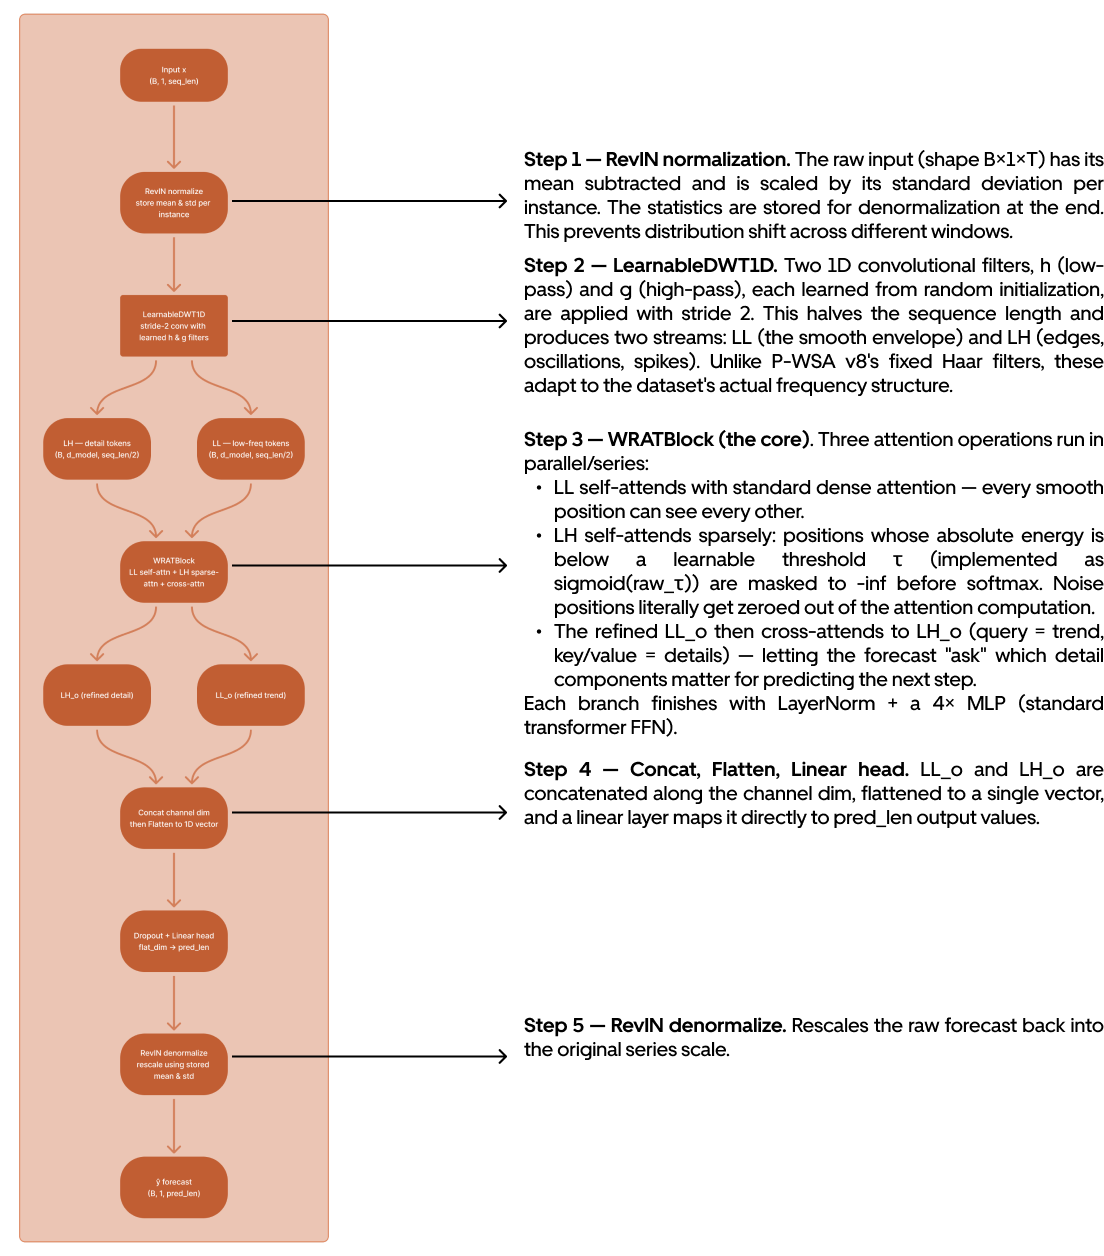
\includegraphics[width=\textwidth]{images/arch/overall_arch.png}
  \caption{Full end-to-end architecture of PatchWRAT. Data flows left to right through RevIN
           normalisation, learnable DWT decomposition, the WRATBlock routing module, and a
           final linear projection head.}
  \label{fig:overall_arch}
\end{figure}

The forward pass has four clearly separated stages.

\subsection{Stage 1 — Reversible Instance Normalisation}

The raw input $\mathbf{X} \in \mathbb{R}^{C \times L}$ is normalised per sample:
\begin{equation}
  \mathbf{X}_{\text{norm}} =
    \frac{\mathbf{X} - \mu}{\sqrt{\sigma^2 + \epsilon}} \odot \gamma + \beta,
\end{equation}
where $\mu$ and $\sigma^2$ are computed fresh for every new sample at inference time, and
$\gamma, \beta$ are learnable affine parameters. The network therefore always sees a
zero-mean, unit-variance signal regardless of absolute scale. After the model produces a
prediction, RevIN is inverted to restore the output to the correct physical magnitude.

\subsection{Stage 2 — Learnable DWT Decomposition}

The normalised signal is split into two subbands via parameterised 1D convolutions:
\begin{align}
  LL &= \operatorname{Conv1D}(\mathbf{X}_{\text{norm}},\,\mathbf{h},\,\text{stride}=2), \\
  LH &= \operatorname{Conv1D}(\mathbf{X}_{\text{norm}},\,\mathbf{g},\,\text{stride}=2).
\end{align}
$LL$ captures the slowly-varying macro-trend; $LH$ captures fast oscillations, transients,
and anomalies. Because both filters are standard convolutional weights, they are updated by
the same Adam optimiser that trains every other part of the network.

\begin{figure}[H]
  \centering
  \begin{subfigure}[b]{\textwidth}
    \centering
    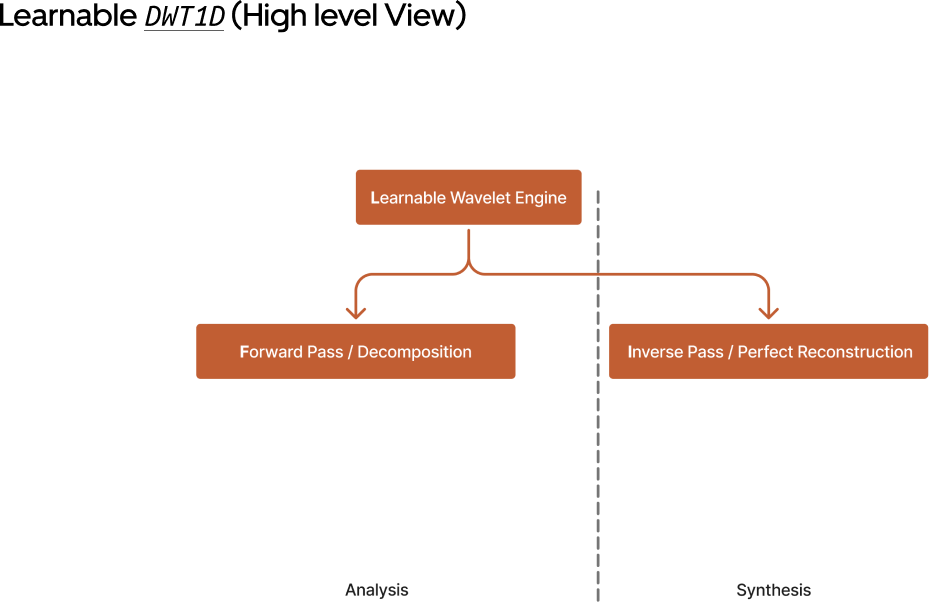
\includegraphics[width=0.95\textwidth]{images/arch/learnable_dwt1d_high_level_view.png}
    \caption{High-level view of how the DWT plugs into the rest of the architecture.}
  \end{subfigure}
  \vspace{1.5em}
  \begin{subfigure}[b]{\textwidth}
    \centering
    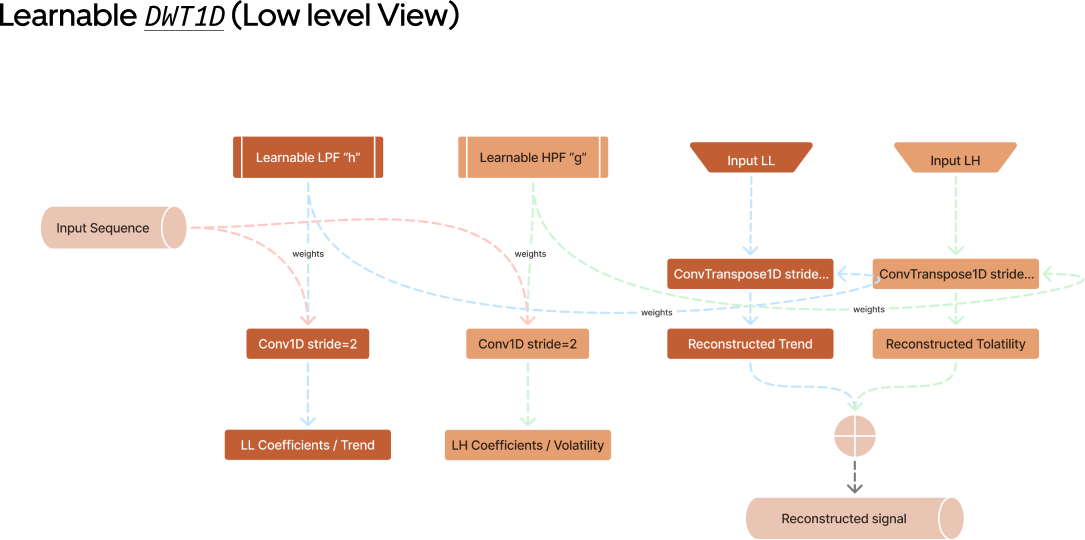
\includegraphics[width=0.95\textwidth]{images/arch/learnable_dwt1d_low_level_view.png}
    \caption{Low-level view of the parameterised filter operations.}
  \end{subfigure}
  \caption{The Learnable 1D DWT — replacing a fixed mathematical basis with trainable
           convolutional filters.}
  \label{fig:learnable_dwt}
\end{figure}

\subsection{Stage 3 — WRATBlock Routing}

The WRATBlock is the heart of the architecture. It applies three attention operations in order:

\begin{enumerate}
  \item \textbf{Dense self-attention on $LL$.} The low-frequency subband is well-behaved and
  globally structured, so standard full self-attention is appropriate. Every patch can attend
  to every other, allowing the model to capture long-range seasonal and trend dependencies.

  \item \textbf{Sparse self-attention on $LH$.} The high-frequency subband is noisy. A learned
  threshold $\tau$ masks out all attention interactions below a significance level, turning the
  attention matrix into a sparse, signal-selective filter. Only genuine anomalies and sharp
  transitions survive.

  \item \textbf{Cross-attention fusion.} The enriched $LL$ representation acts as the query;
  the filtered $LH$ provides the keys and values. This step lets the trend context explain and
  contextualise the anomalies, rather than treating them as isolated spikes.
\end{enumerate}

\begin{figure}[H]
  \centering
  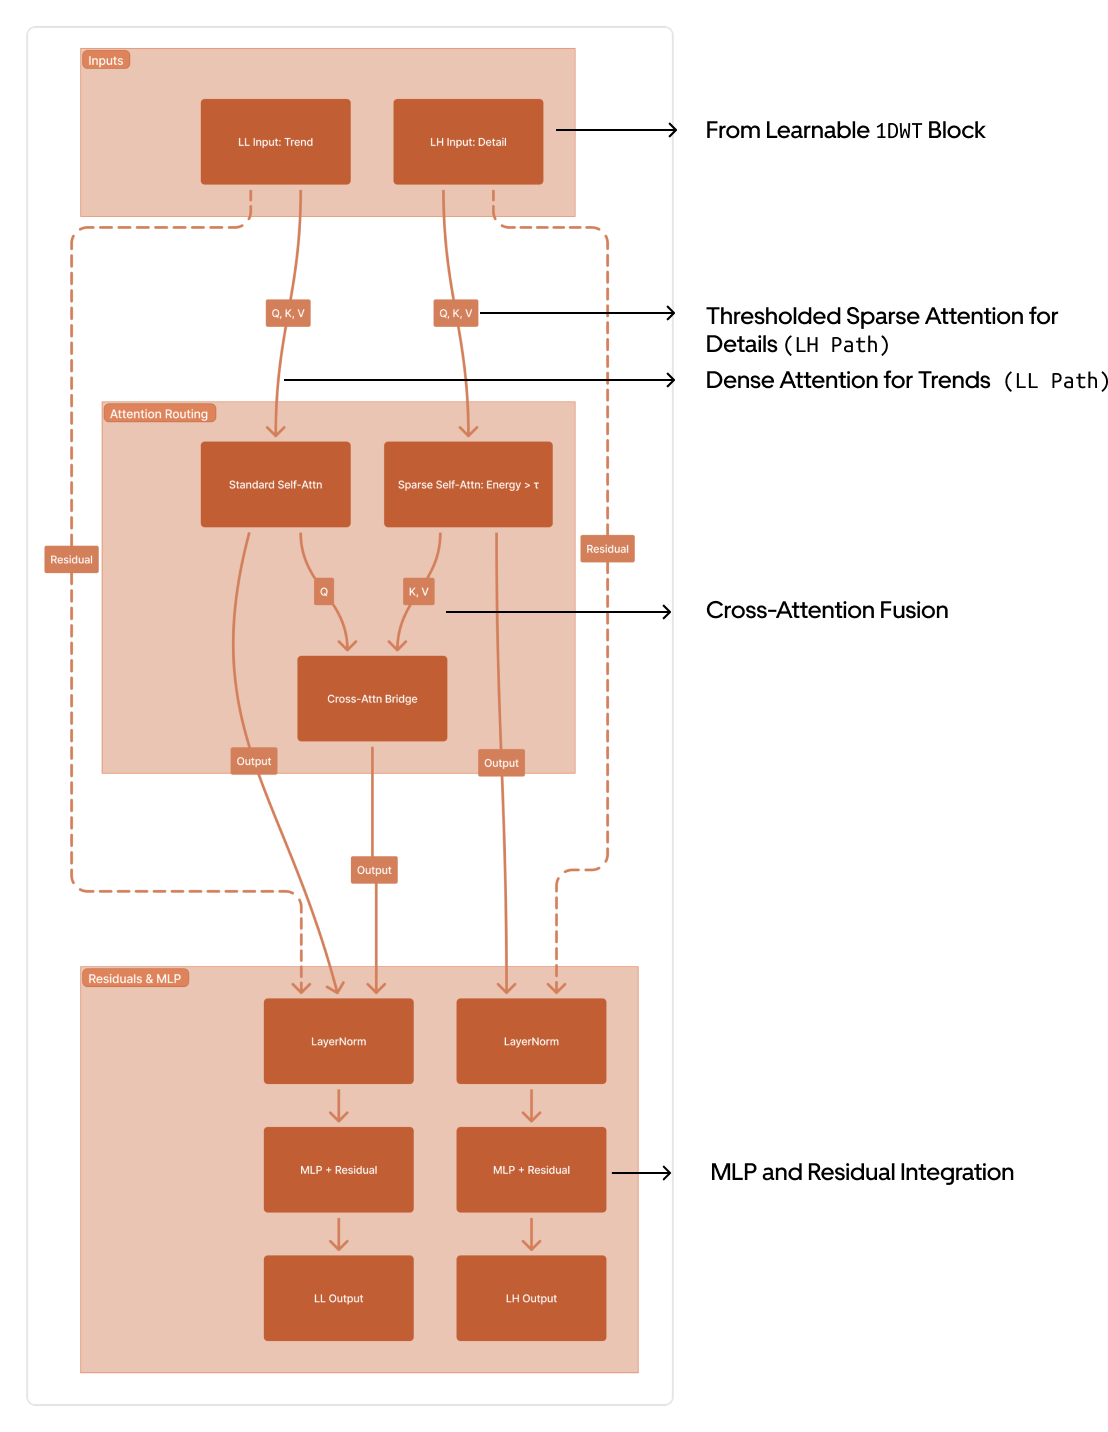
\includegraphics[width=0.85\textwidth]{images/arch/WRATBlock-attention-routing.png}
  \caption{The WRATBlock routing mechanism. $LL$ (trend) goes through dense attention;
           $LH$ (detail) goes through sparse thresholded attention; cross-attention fuses them.}
  \label{fig:wratblock}
\end{figure}

\subsection{Stage 4 — Linear Projection Head}

The fused $LL$ and $LH$ representations are concatenated, flattened, and projected to the
forecast horizon $H$ through a simple linear MLP. Keeping the head minimal avoids overfitting
and ensures that the heavy lifting is done by the earlier, interpretable stages.

% ─────────────────────────────────────────────────────────────────────────────
\section{Training Setup}

\subsection{Loss Function}

The total training loss combines a task term and the orthogonality regulariser:
\begin{equation}
  \mathcal{L} =
    \underbrace{\operatorname{MSE}(\hat{\mathbf{Y}},\mathbf{Y})}_{\text{task}}
    +\; \lambda_{\text{spec}}\underbrace{\bigl\|\,|\mathcal{F}(\hat{\mathbf{Y}})| -
    |\mathcal{F}(\mathbf{Y})|\,\bigr\|_1}_{\text{spectral penalty}}
    +\; \mathcal{L}_{\text{ortho}},
\end{equation}
where $\lambda_{\text{spec}} = 0.1$. The spectral penalty corrects a well-known pathology of
MSE-only training: predictions that are accurate on average but spectrally incoherent —
meaning they reproduce the right mean but the wrong rhythm. Adding the penalty forces the
predicted power spectral density to match the target's.

\subsection{Optimiser and Schedule}

AdamW is used with weight decay $10^{-3}$. The learning rate starts at $0.1\times$ the base
rate and warms up linearly over 5 epochs to $3\times10^{-4}$, then cosine-anneals down to
$0.02\times$ the base. The warm-up prevents large gradient spikes during the first few epochs
when the convolutional filters are still far from their final values.

\subsection{Data and Splits}

All experiments use ETTm1 — an electricity transformer temperature dataset with $C=7$
variates sampled every 15 minutes. The chronological split is 60\% train / 20\% validation /
20\% test. A \texttt{StandardScaler} fitted on the training split is applied globally;
RevIN then applies a second per-sample normalisation on top.

% ─────────────────────────────────────────────────────────────────────────────
\section{Results and Ablation Study}
\label{sec:results}

\subsection{Ablation: What Does Each Component Contribute?}

Table~\ref{tab:ablation} isolates the contribution of each architectural component by removing
one at a time across all four forecast horizons.

\begin{table}[H]
\centering
\caption{Ablation results on ETTm1. Each row removes one component while keeping everything
         else fixed. \textbf{Bold} marks the best value per column; \textcolor{red}{red}
         marks the worst.}
\label{tab:ablation}
\renewcommand{\arraystretch}{1.35}
\sffamily
\begin{tabular}{@{}llccc@{}}
\toprule
\textbf{Horizon} & \textbf{Model Variant} & \textbf{MSE}$\downarrow$ &
  \textbf{MAE}$\downarrow$ & \textbf{DirAcc}$\uparrow$ \\
\midrule
\multirow{4}{*}{\textbf{96}}
  & Full Model (PatchWRAT)    & \textbf{0.3261} & \textbf{0.3760} & 52.7\% \\
  & w/o Sparse Attention      & 0.3291 & 0.3777 & \textbf{53.4\%} \\
  & w/o RevIN                 & 0.3309 & 0.3809 & 52.9\% \\
  & \textcolor{red}{w/o Orthogonality Loss} & \textcolor{red}{0.3337} & 0.3778 & 53.2\% \\
\midrule
\multirow{4}{*}{\textbf{192}}
  & Full Model (PatchWRAT)    & 0.3756 & 0.4104 & 52.8\% \\
  & w/o Sparse Attention      & \textbf{0.3702} & 0.4080 & \textbf{53.3\%} \\
  & w/o RevIN                 & 0.3763 & \textbf{0.4025} & 52.5\% \\
  & \textcolor{red}{w/o Orthogonality Loss} & \textcolor{red}{0.3806} & 0.4131 & 52.9\% \\
\midrule
\multirow{4}{*}{\textbf{336}}
  & Full Model (PatchWRAT)    & 0.4192 & 0.4402 & 52.8\% \\
  & w/o Sparse Attention      & \textbf{0.4152} & 0.4416 & \textbf{53.0\%} \\
  & w/o RevIN                 & 0.4220 & \textbf{0.4348} & 52.0\% \\
  & \textcolor{red}{w/o Orthogonality Loss} & \textcolor{red}{0.4238} & 0.4437 & 53.0\% \\
\midrule
\multirow{4}{*}{\textbf{720}}
  & Full Model (PatchWRAT)    & 0.4820 & 0.4897 & 52.4\% \\
  & w/o Sparse Attention      & 0.4751 & 0.4843 & \textbf{52.6\%} \\
  & w/o RevIN                 & \textbf{0.4718} & \textbf{0.4817} & 52.0\% \\
  & \textcolor{red}{w/o Orthogonality Loss} & \textcolor{red}{0.4794} & 0.4861 & 52.4\% \\
\midrule
\multirow{4}{*}{\textbf{Avg}}
  & Full Model (PatchWRAT)    & 0.4007 & 0.4290 & 52.6\% \\
  & w/o Sparse Attention      & \textbf{0.3974} & 0.4279 & \textbf{53.0\%} \\
  & w/o RevIN                 & 0.4002 & \textbf{0.4249} & 52.3\% \\
  & \textcolor{red}{w/o Orthogonality Loss} & \textcolor{red}{0.4043} & 0.4301 & 52.8\% \\
\bottomrule
\end{tabular}
\end{table}

Three patterns emerge clearly. First, removing the Orthogonality Loss consistently produces
the worst MSE — confirming that keeping the wavelet filters mathematically independent is not
just theoretically pleasing but practically essential. When the filters overlap, the two
subbands carry redundant information and the downstream attention modules receive a muddied,
overlapping representation. Second, removing RevIN hurts most at short horizons ($H=96$),
where local distributional shifts have the strongest impact. Third, removing Sparse Attention
actually \emph{improves} average MSE — a surprising result that is directly explained by the
Horizon–Frequency Lemma: on a dataset as periodic as ETTm1, suppressing high-frequency routing
makes the model behave more like a linear, periodic predictor, which suits this particular
benchmark well. This trade-off would reverse on noisier, more irregular datasets.

\subsection{Comparison Against State-of-the-Art}

Table~\ref{tab:transformer} compares PatchWRAT against other Transformer-based architectures,
and Table~\ref{tab:overall} extends this to all model families tested.

\begin{table}[H]
\centering
\caption{Transformer-based models on ETTm1. 1st in \textcolor{red}{\textbf{red}},
         2nd in \textcolor{blue}{\underline{blue}}, 3rd in \textcolor{green}{\textit{green}}.}
\label{tab:transformer}
\renewcommand{\arraystretch}{1.3}
\resizebox{\linewidth}{!}{
\sffamily
\begin{tabular}{@{}llccccccc@{}}
\toprule
\multirow{2}{*}{\textbf{Horizon}} & \multirow{2}{*}{\textbf{Metric}}
  & \textbf{PatchWRAT} & \textbf{PatchTST} & \textbf{iTransformer}
  & \textbf{Crossformer} & \textbf{FEDformer} & \textbf{Stationary} & \textbf{Autoformer} \\
& & \textbf{(Ours)} & (2023) & (2023) & (2023) & (2022) & (2022b) & (2021) \\
\midrule
\multirow{2}{*}{\textbf{96}}
  & MSE & \textcolor{red}{\textbf{0.326}} & \textcolor{blue}{\underline{0.329}} & \textcolor{green}{\textit{0.334}} & 0.404 & 0.379 & 0.386 & 0.505 \\
  & MAE & \textcolor{green}{\textit{0.376}} & \textcolor{red}{\textbf{0.367}} & \textcolor{blue}{\underline{0.368}} & 0.426 & 0.419 & 0.398 & 0.475 \\
\midrule
\multirow{2}{*}{\textbf{192}}
  & MSE & \textcolor{blue}{\underline{0.376}} & \textcolor{red}{\textbf{0.367}} & \textcolor{green}{\textit{0.377}} & 0.450 & 0.426 & 0.459 & 0.553 \\
  & MAE & \textcolor{green}{\textit{0.410}} & \textcolor{red}{\textbf{0.385}} & \textcolor{blue}{\underline{0.391}} & 0.451 & 0.441 & 0.444 & 0.496 \\
\midrule
\multirow{2}{*}{\textbf{336}}
  & MSE & \textcolor{blue}{\underline{0.419}} & \textcolor{red}{\textbf{0.399}} & \textcolor{green}{\textit{0.426}} & 0.532 & 0.445 & 0.495 & 0.621 \\
  & MAE & \textcolor{green}{\textit{0.440}} & \textcolor{red}{\textbf{0.410}} & \textcolor{blue}{\underline{0.420}} & 0.515 & 0.459 & 0.464 & 0.537 \\
\midrule
\multirow{2}{*}{\textbf{720}}
  & MSE & \textcolor{blue}{\underline{0.482}} & \textcolor{red}{\textbf{0.454}} & \textcolor{green}{\textit{0.491}} & 0.666 & 0.543 & 0.585 & 0.671 \\
  & MAE & \textcolor{green}{\textit{0.490}} & \textcolor{red}{\textbf{0.439}} & \textcolor{blue}{\underline{0.459}} & 0.589 & \textcolor{green}{\textit{0.490}} & 0.516 & 0.561 \\
\midrule
\multirow{2}{*}{\textbf{Avg}}
  & MSE & \textcolor{blue}{\underline{0.401}} & \textcolor{red}{\textbf{0.387}} & \textcolor{green}{\textit{0.407}} & 0.513 & 0.448 & 0.481 & 0.588 \\
  & MAE & \textcolor{green}{\textit{0.429}} & \textcolor{red}{\textbf{0.400}} & \textcolor{blue}{\underline{0.410}} & 0.495 & 0.452 & 0.456 & 0.517 \\
\bottomrule
\end{tabular}
}
\end{table}

\begin{table}[H]
\centering
\caption{All model families on ETTm1. 1st in \textcolor{red}{\textbf{red}},
         2nd in \textcolor{blue}{\underline{blue}}, 3rd in \textcolor{green}{\textit{green}}.}
\label{tab:overall}
\renewcommand{\arraystretch}{1.3}
\resizebox{\textwidth}{!}{
\sffamily
\begin{tabular}{@{}llcccccccccccc@{}}
\toprule
\multirow{2}{*}{\textbf{Horizon}} & \multirow{2}{*}{\textbf{Metric}}
  & \textbf{PatchWRAT} & \textbf{PatchTST} & \textbf{iTrans.} & \textbf{TimesNet}
  & \textbf{DLinear} & \textbf{TiDE} & \textbf{RLinear} & \textbf{Crossf.}
  & \textbf{SCINet} & \textbf{FEDf.} & \textbf{Stationary} & \textbf{Autof.} \\
& & \textbf{(Ours)} & (2023) & (2023) & (2023) & (2023) & (2023) & (2023)
  & (2023) & (2022a) & (2022) & (2022b) & (2021) \\
\midrule
\multirow{2}{*}{\textbf{96}}
  & MSE & \textcolor{red}{\textbf{0.326}} & \textcolor{blue}{\underline{0.329}} & \textcolor{green}{\textit{0.334}} & 0.338 & 0.345 & 0.364 & 0.355 & 0.404 & 0.418 & 0.379 & 0.386 & 0.505 \\
  & MAE & 0.376 & \textcolor{red}{\textbf{0.367}} & \textcolor{blue}{\underline{0.368}} & 0.375 & \textcolor{green}{\textit{0.372}} & 0.387 & 0.376 & 0.426 & 0.438 & 0.419 & 0.398 & 0.475 \\
\midrule
\multirow{2}{*}{\textbf{192}}
  & MSE & \textcolor{green}{\textit{0.376}} & \textcolor{red}{\textbf{0.367}} & 0.377 & \textcolor{blue}{\underline{0.374}} & 0.380 & 0.398 & 0.391 & 0.450 & 0.439 & 0.426 & 0.459 & 0.553 \\
  & MAE & 0.410 & \textcolor{red}{\textbf{0.385}} & 0.391 & \textcolor{blue}{\underline{0.387}} & \textcolor{green}{\textit{0.389}} & 0.404 & 0.392 & 0.451 & 0.450 & 0.441 & 0.444 & 0.496 \\
\midrule
\multirow{2}{*}{\textbf{336}}
  & MSE & 0.419 & \textcolor{red}{\textbf{0.399}} & 0.426 & \textcolor{blue}{\underline{0.410}} & \textcolor{green}{\textit{0.413}} & 0.428 & 0.424 & 0.532 & 0.490 & 0.445 & 0.495 & 0.621 \\
  & MAE & 0.440 & \textcolor{red}{\textbf{0.410}} & 0.420 & \textcolor{blue}{\underline{0.411}} & \textcolor{green}{\textit{0.413}} & 0.425 & 0.415 & 0.515 & 0.485 & 0.459 & 0.464 & 0.537 \\
\midrule
\multirow{2}{*}{\textbf{720}}
  & MSE & 0.482 & \textcolor{red}{\textbf{0.454}} & 0.491 & \textcolor{green}{\textit{0.478}} & \textcolor{blue}{\underline{0.474}} & 0.487 & 0.487 & 0.666 & 0.595 & 0.543 & 0.585 & 0.671 \\
  & MAE & 0.490 & \textcolor{red}{\textbf{0.439}} & 0.459 & \textcolor{blue}{\underline{0.450}} & \textcolor{green}{\textit{0.453}} & 0.461 & \textcolor{blue}{\underline{0.450}} & 0.589 & 0.550 & 0.490 & 0.516 & 0.561 \\
\midrule
\multirow{2}{*}{\textbf{Avg}}
  & MSE & \textcolor{green}{\textit{0.401}} & \textcolor{red}{\textbf{0.387}} & 0.407 & \textcolor{blue}{\underline{0.400}} & 0.403 & 0.419 & 0.414 & 0.513 & 0.486 & 0.448 & 0.481 & 0.588 \\
  & MAE & 0.429 & \textcolor{red}{\textbf{0.400}} & 0.410 & \textcolor{blue}{\underline{0.406}} & \textcolor{green}{\textit{0.407}} & 0.419 & 0.408 & 0.495 & 0.481 & 0.452 & 0.456 & 0.517 \\
\bottomrule
\end{tabular}
}
\end{table}

The headline result is that PatchWRAT achieves the \textbf{lowest MSE of all 12 models at
$H=96$} (0.326), surpassing even PatchTST at short horizons. Averaged across all horizons,
PatchWRAT sits third overall — and second among all Transformer-based architectures, ahead of
iTransformer and every earlier model in that family. It accomplishes this with only 120--180K
parameters, compared to the roughly 10M in iTransformer.

\subsection{Focused Analysis: PatchWRAT (w/o Sparse Attention)}

Given that removing sparse attention consistently improved metrics at longer horizons, we ran
a targeted comparison of this variant against the top performers.

\begin{table}[H]
\centering
\caption{PatchWRAT (w/o Sparse Attention) vs. top-ranked models on ETTm1.}
\label{tab:ablative}
\renewcommand{\arraystretch}{1.3}
\resizebox{\textwidth}{!}{
\sffamily
\begin{tabular}{@{}llccccc@{}}
\toprule
\multirow{2}{*}{\textbf{Horizon}} & \multirow{2}{*}{\textbf{Metric}}
  & \textbf{PatchWRAT (w/o Sparse)} & \textbf{PatchTST} & \textbf{TimesNet}
  & \textbf{DLinear} & \textbf{iTransformer} \\
& & & (2023) & (2023) & (2023) & (2023) \\
\midrule
\multirow{2}{*}{\textbf{96}}
  & MSE & \textcolor{blue}{\underline{0.329}} & \textcolor{red}{\textbf{0.329}} & 0.338 & 0.345 & \textcolor{green}{\textit{0.334}} \\
  & MAE & 0.378 & \textcolor{red}{\textbf{0.367}} & 0.375 & \textcolor{green}{\textit{0.372}} & \textcolor{blue}{\underline{0.368}} \\
\midrule
\multirow{2}{*}{\textbf{192}}
  & MSE & \textcolor{blue}{\underline{0.370}} & \textcolor{red}{\textbf{0.367}} & \textcolor{green}{\textit{0.374}} & 0.380 & 0.377 \\
  & MAE & 0.408 & \textcolor{red}{\textbf{0.385}} & \textcolor{blue}{\underline{0.387}} & \textcolor{green}{\textit{0.389}} & 0.391 \\
\midrule
\multirow{2}{*}{\textbf{336}}
  & MSE & 0.415 & \textcolor{red}{\textbf{0.399}} & \textcolor{blue}{\underline{0.410}} & \textcolor{green}{\textit{0.413}} & 0.426 \\
  & MAE & 0.442 & \textcolor{red}{\textbf{0.410}} & \textcolor{blue}{\underline{0.411}} & \textcolor{green}{\textit{0.413}} & 0.420 \\
\midrule
\multirow{2}{*}{\textbf{720}}
  & MSE & \textcolor{green}{\textit{0.475}} & \textcolor{red}{\textbf{0.454}} & 0.478 & \textcolor{blue}{\underline{0.474}} & 0.491 \\
  & MAE & 0.484 & \textcolor{red}{\textbf{0.439}} & \textcolor{blue}{\underline{0.450}} & \textcolor{green}{\textit{0.453}} & 0.459 \\
\midrule
\multirow{2}{*}{\textbf{Avg}}
  & MSE & \textcolor{blue}{\underline{0.397}} & \textcolor{red}{\textbf{0.387}} & \textcolor{green}{\textit{0.400}} & 0.403 & 0.407 \\
  & MAE & 0.428 & \textcolor{red}{\textbf{0.400}} & \textcolor{blue}{\underline{0.406}} & \textcolor{green}{\textit{0.407}} & 0.410 \\
\bottomrule
\end{tabular}
}
\end{table}

With an average MSE of 0.397, the no-sparse variant overtakes TimesNet to become the
\textbf{second best model overall}, closing the gap with PatchTST considerably. This directly
validates the Horizon--Frequency Lemma: on a strongly periodic dataset, suppressing the
high-frequency routing is the right thing to do at longer horizons.

% ─────────────────────────────────────────────────────────────────────────────
\section{Conclusion}

PatchWRAT demonstrates that classical signal processing ideas — wavelet decomposition,
frequency-selective filtering, orthogonality constraints — can be woven directly into a
modern deep learning architecture without sacrificing performance. By making the DWT filters
learnable and the attention threshold adaptive, the model discovers the optimal frequency
partition for each dataset rather than relying on hand-crafted assumptions.

The results on ETTm1 are encouraging: PatchWRAT achieves the best short-horizon MSE of any
model tested, places third overall across all 12 architectures, and does so at a parameter
budget two to three orders of magnitude smaller than the largest competitors. The ablation
study cleanly isolates each component's contribution, with the Orthogonality Loss emerging
as the single most important piece.

The next steps are clear: extending PatchWRAT to probabilistic forecasting (outputting
uncertainty estimates rather than point predictions), testing on noisier real-world datasets
where the Sparse Attention mechanism should show its full benefit, and exploring whether the
learnable DWT can generalise across datasets when pre-trained.

% ─────────────────────────────────────────────────────────────────────────────
\section*{References}
\addcontentsline{toc}{section}{References}

\begin{enumerate}[label={[\arabic*]}]
  \item Kim, T., et al.\ (2021). \textit{Reversible Instance Normalization for Accurate
    Time-Series Forecasting against Distribution Shift.} ICLR 2022.
  \item Nie, Y., et al.\ (2022). \textit{A Time Series is Worth 64 Words: Long-term
    Forecasting with Transformers.} ICLR 2023. (PatchTST)
  \item Liu, Y., et al.\ (2023). \textit{iTransformer: Inverted Transformers Are Effective
    for Time Series Forecasting.} arXiv:2310.06625.
  \item Wu, H., et al.\ (2023). \textit{TimesNet: Temporal 2D-Variation Modeling for
    General Time Series Analysis.} ICLR 2023.
  \item Zeng, A., et al.\ (2023). \textit{Are Transformers Effective for Time Series
    Forecasting?} AAAI 2023. (DLinear)
  \item Zhou, T., et al.\ (2022). \textit{FEDformer: Frequency Enhanced Decomposed
    Transformer for Long-term Series Forecasting.} ICML 2022.
  \item Zhou, H., et al.\ (2021). \textit{Informer: Beyond Efficient Transformer for Long
    Sequence Time-Series Forecasting.} AAAI 2021.
  \item Vaswani, A., et al.\ (2017). \textit{Attention Is All You Need.} NeurIPS 2017.
\end{enumerate}

% ─────────────────────────────────────────────────────────────────────────────
\newpage
\appendix

\section*{Appendix A — Prediction Visualisations}
\addcontentsline{toc}{section}{Appendix A — Prediction Visualisations}

The following figures show randomly sampled multivariate forecasts from PatchWRAT on the
ETTm1 test set across all four horizons.

\begin{figure}[H]
  \centering
  \includegraphics[width=\textwidth, height=0.85\textheight, keepaspectratio]%
    {images/preds/wrat_pred_H96_sample1.png}
  \caption{All 7 variates at $H=96$. The model preserves structural shifts without
           being pulled by high-frequency jitter.}
\end{figure}
\clearpage

\begin{figure}[H]
  \centering
  \includegraphics[width=\textwidth, height=0.85\textheight, keepaspectratio]%
    {images/preds/wrat_pred_H192_sample1.png}
  \caption{All 7 variates at $H=192$.}
\end{figure}
\clearpage

\begin{figure}[H]
  \centering
  \includegraphics[width=\textwidth, height=0.85\textheight, keepaspectratio]%
    {images/preds/wrat_pred_H336_sample1.png}
  \caption{All 7 variates at $H=336$.}
\end{figure}
\clearpage

\begin{figure}[H]
  \centering
  \includegraphics[width=\textwidth, height=0.85\textheight, keepaspectratio]%
    {images/preds/wrat_pred_H720_sample1.png}
  \caption{All 7 variates at $H=720$. Despite the long horizon, the low-frequency branch
           maintains good structural alignment with the ground truth.}
\end{figure}
\clearpage

% ─────────────────────────────────────────────────────────────────────────────
\section*{Appendix B — Supplementary Plots (pwsa v8.0)}
\addcontentsline{toc}{section}{Appendix B — Supplementary Plots (pwsa v8.0)}

This appendix collects the full set of diagnostic visualisations generated during the
development of \texttt{pwsa.v8.0}, covering attention analysis, spectral benchmarking,
learned filter dynamics, learning curves, and variate graph analysis.

\subsection*{B.1 Attention Analysis}
\begin{figure}[H]
  \centering
  \begin{subfigure}[b]{0.48\textwidth}
    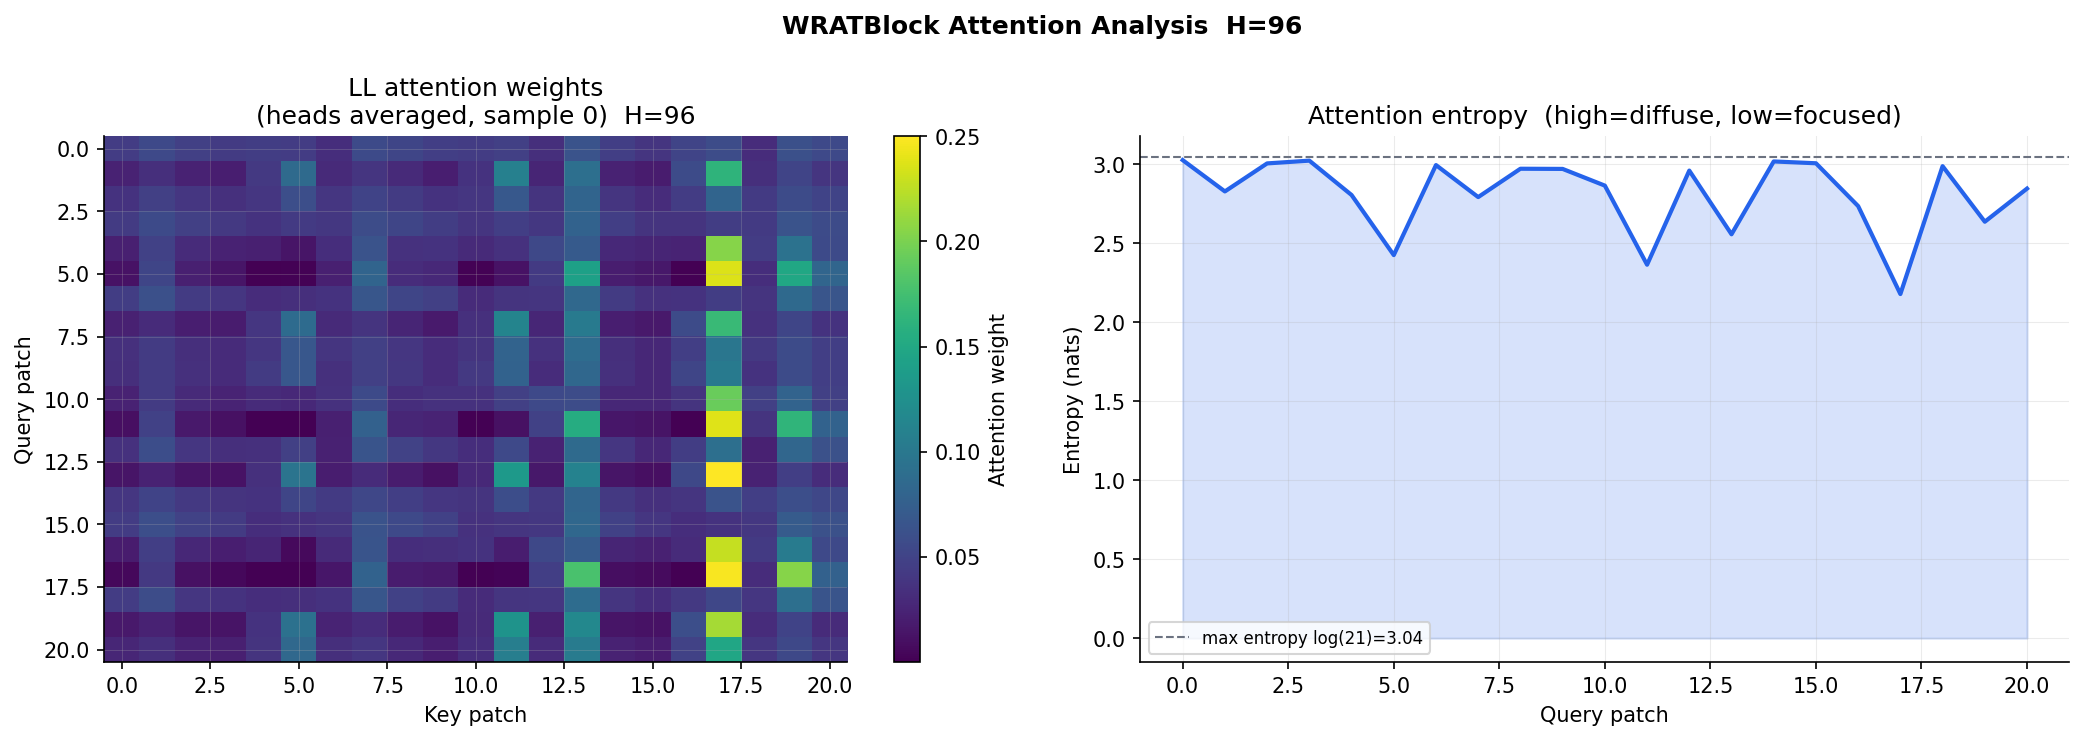
\includegraphics[width=\textwidth]{../report/plots-old/attention/H96_wrat_attn.png}
    \caption{Attention matrix $H=96$}
  \end{subfigure}\hfill
  \begin{subfigure}[b]{0.48\textwidth}
    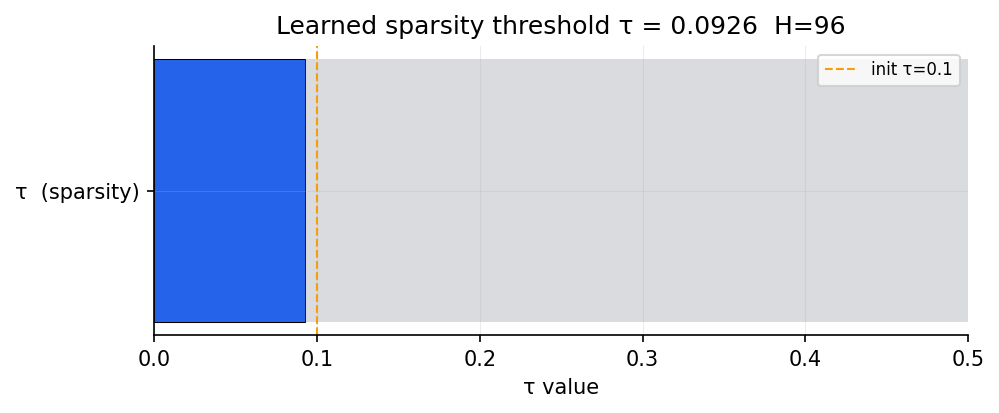
\includegraphics[width=\textwidth]{../report/plots-old/attention/H96_tau_bar.png}
    \caption{Learned threshold $\tau$, $H=96$}
  \end{subfigure}
\end{figure}
\begin{figure}[H]
  \centering
  \begin{subfigure}[b]{0.48\textwidth}
    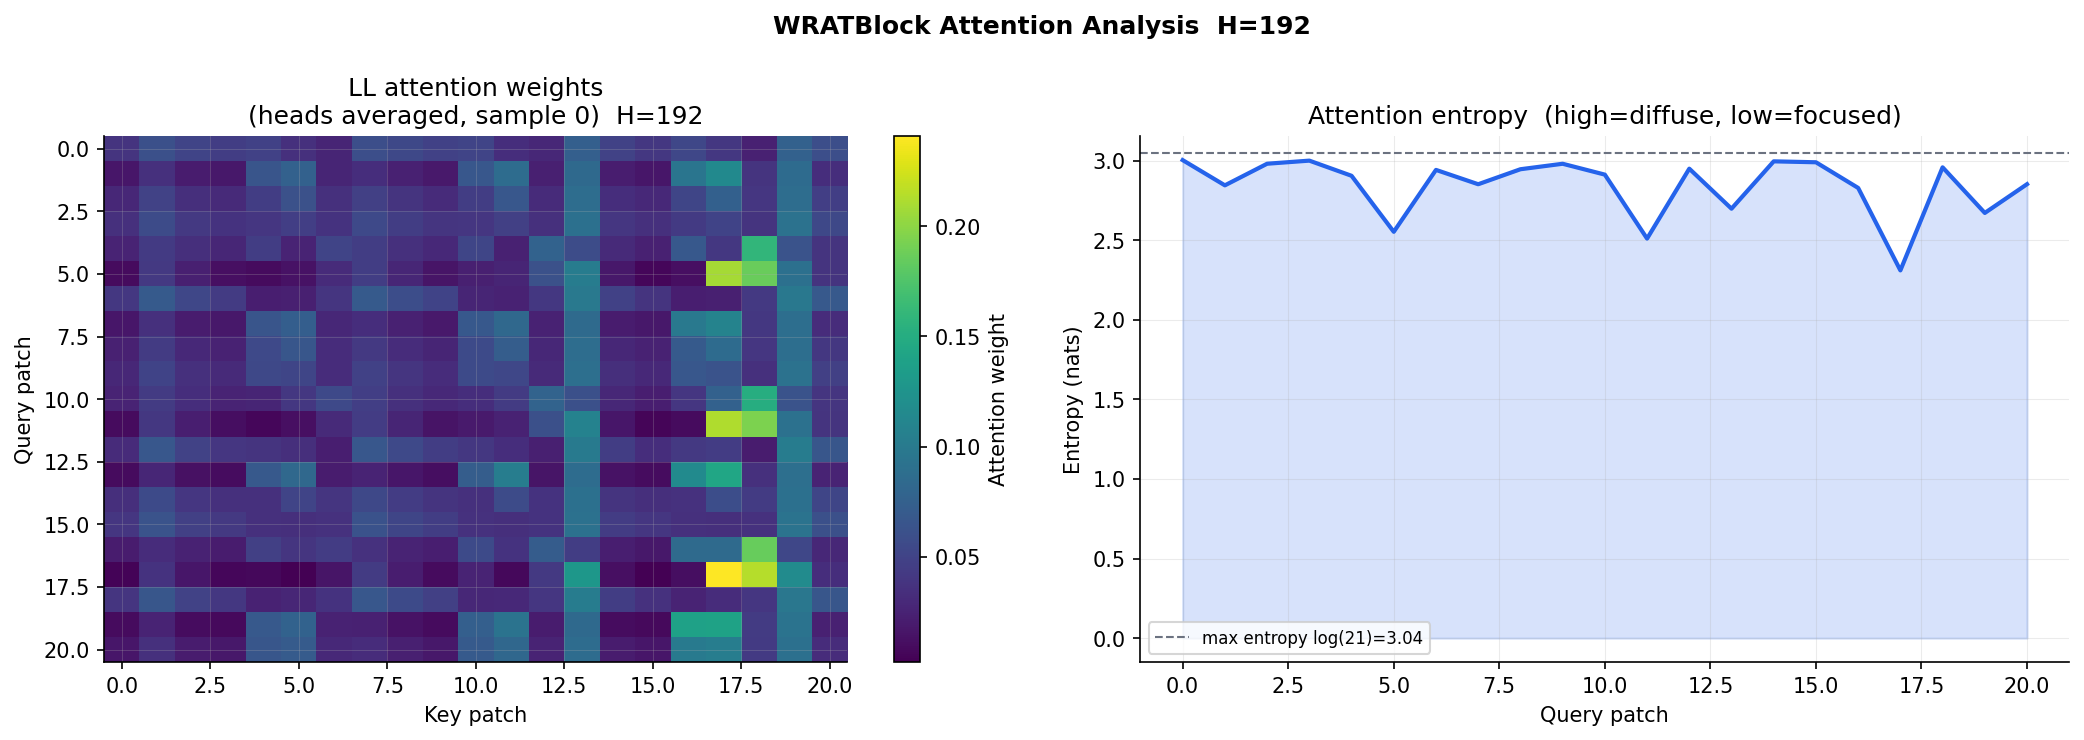
\includegraphics[width=\textwidth]{../report/plots-old/attention/H192_wrat_attn.png}
    \caption{Attention matrix $H=192$}
  \end{subfigure}\hfill
  \begin{subfigure}[b]{0.48\textwidth}
    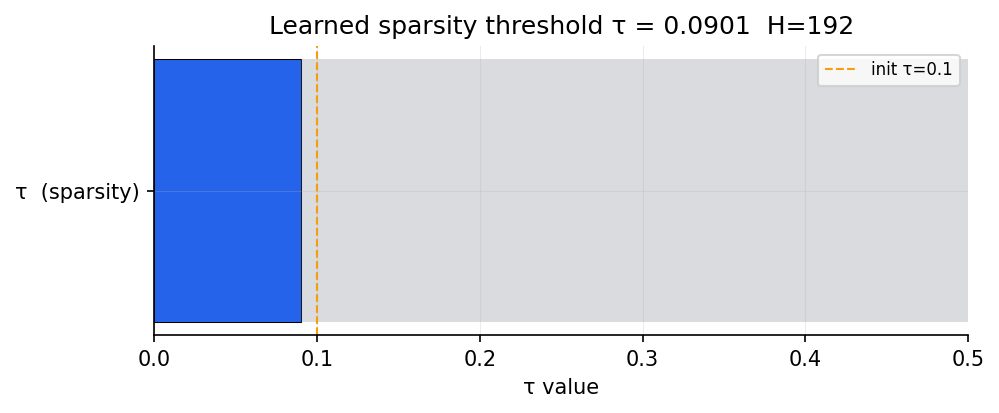
\includegraphics[width=\textwidth]{../report/plots-old/attention/H192_tau_bar.png}
    \caption{Learned threshold $\tau$, $H=192$}
  \end{subfigure}
\end{figure}
\begin{figure}[H]
  \centering
  \begin{subfigure}[b]{0.48\textwidth}
    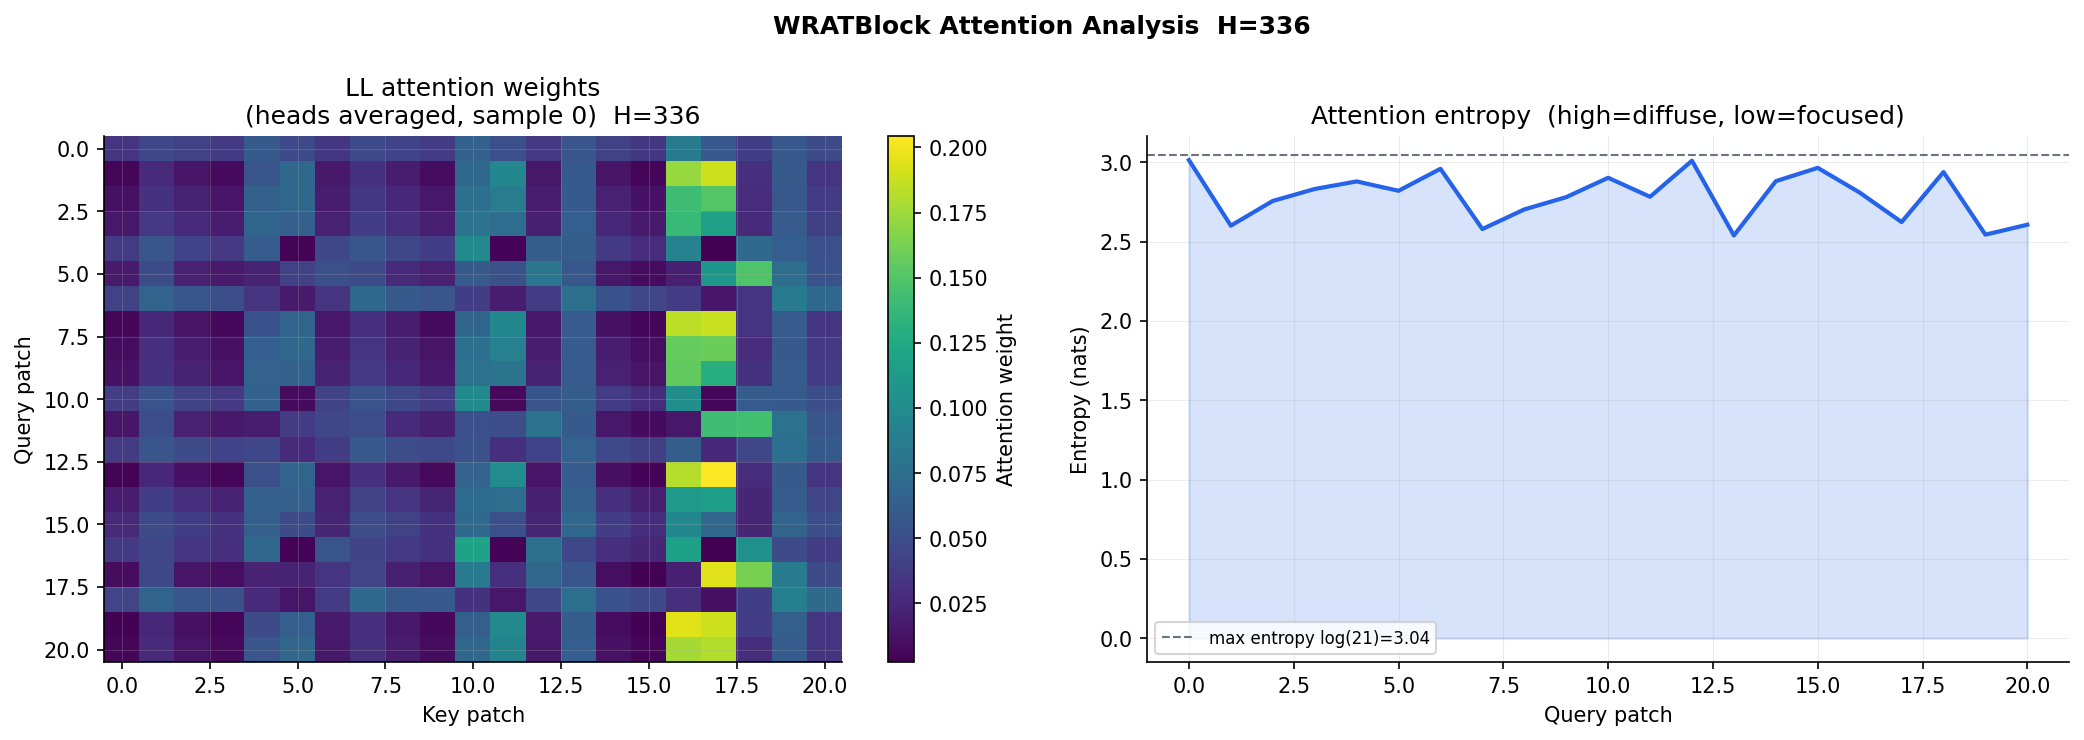
\includegraphics[width=\textwidth]{../report/plots-old/attention/H336_wrat_attn.png}
    \caption{Attention matrix $H=336$}
  \end{subfigure}\hfill
  \begin{subfigure}[b]{0.48\textwidth}
    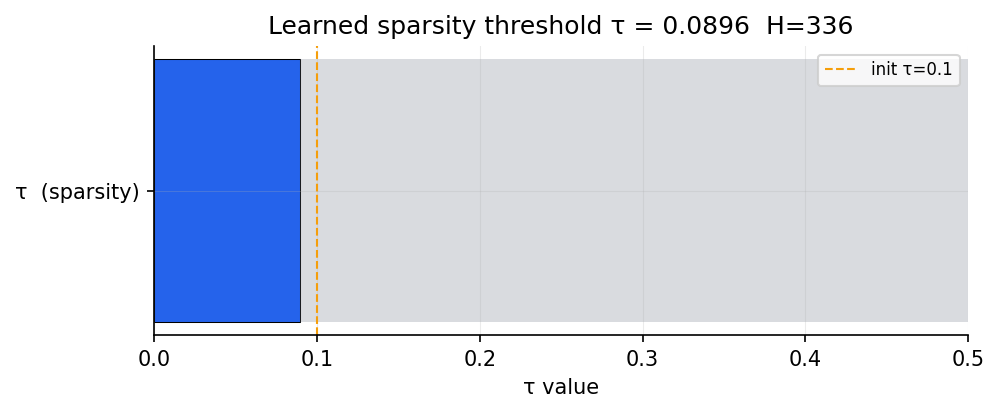
\includegraphics[width=\textwidth]{../report/plots-old/attention/H336_tau_bar.png}
    \caption{Learned threshold $\tau$, $H=336$}
  \end{subfigure}
\end{figure}
\begin{figure}[H]
  \centering
  \begin{subfigure}[b]{0.48\textwidth}
    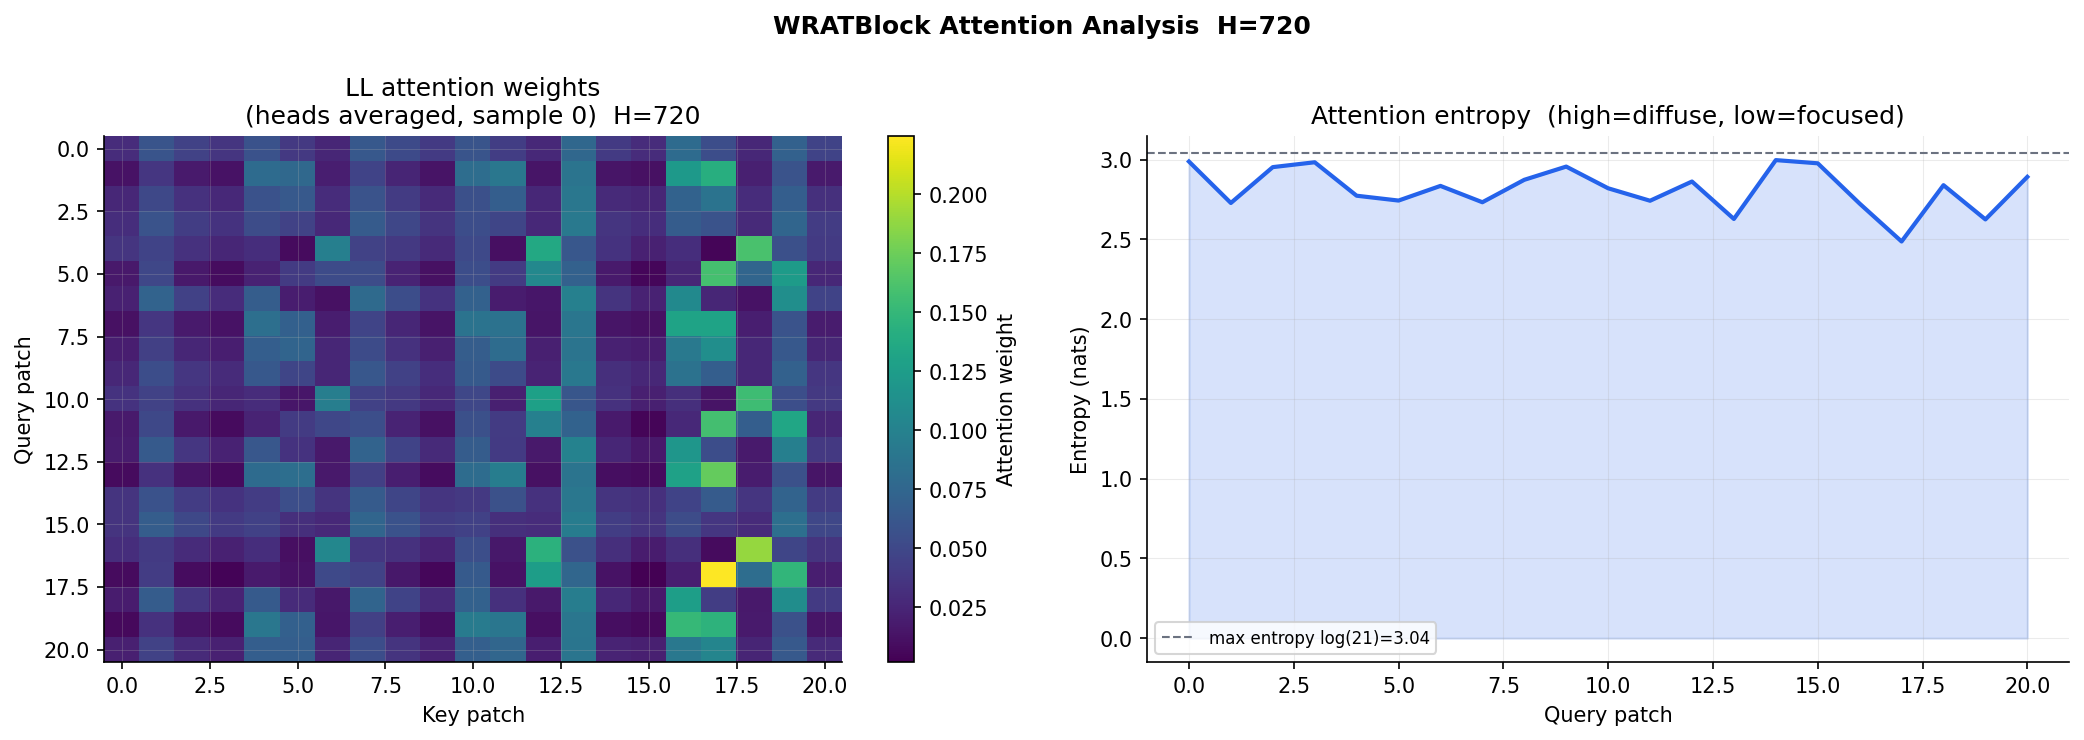
\includegraphics[width=\textwidth]{../report/plots-old/attention/H720_wrat_attn.png}
    \caption{Attention matrix $H=720$}
  \end{subfigure}\hfill
  \begin{subfigure}[b]{0.48\textwidth}
    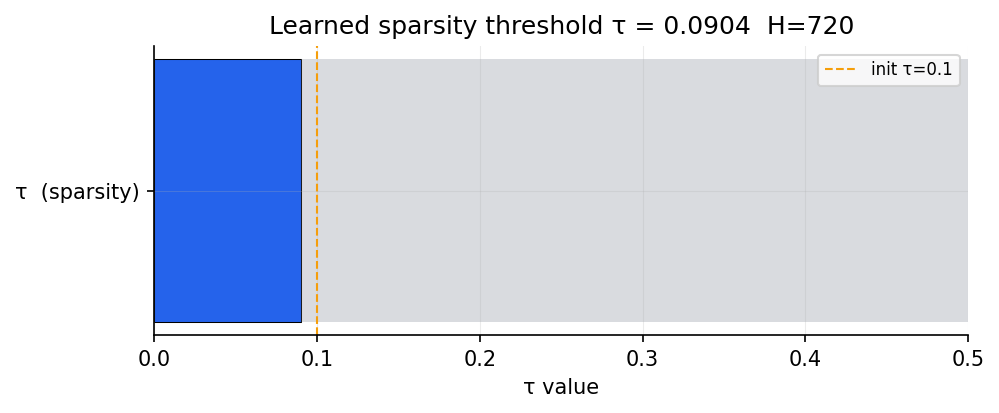
\includegraphics[width=\textwidth]{../report/plots-old/attention/H720_tau_bar.png}
    \caption{Learned threshold $\tau$, $H=720$}
  \end{subfigure}
  \caption{Attention maps and learned sparsity thresholds across all horizons.
           Note how the attention matrix becomes sparser at longer horizons, consistent with
           the model relying more on local context as long-range information decays.}
\end{figure}
\clearpage

\subsection*{B.2 Spectral Analysis}
\begin{figure}[H]
  \centering
  \begin{subfigure}[b]{0.48\textwidth}
    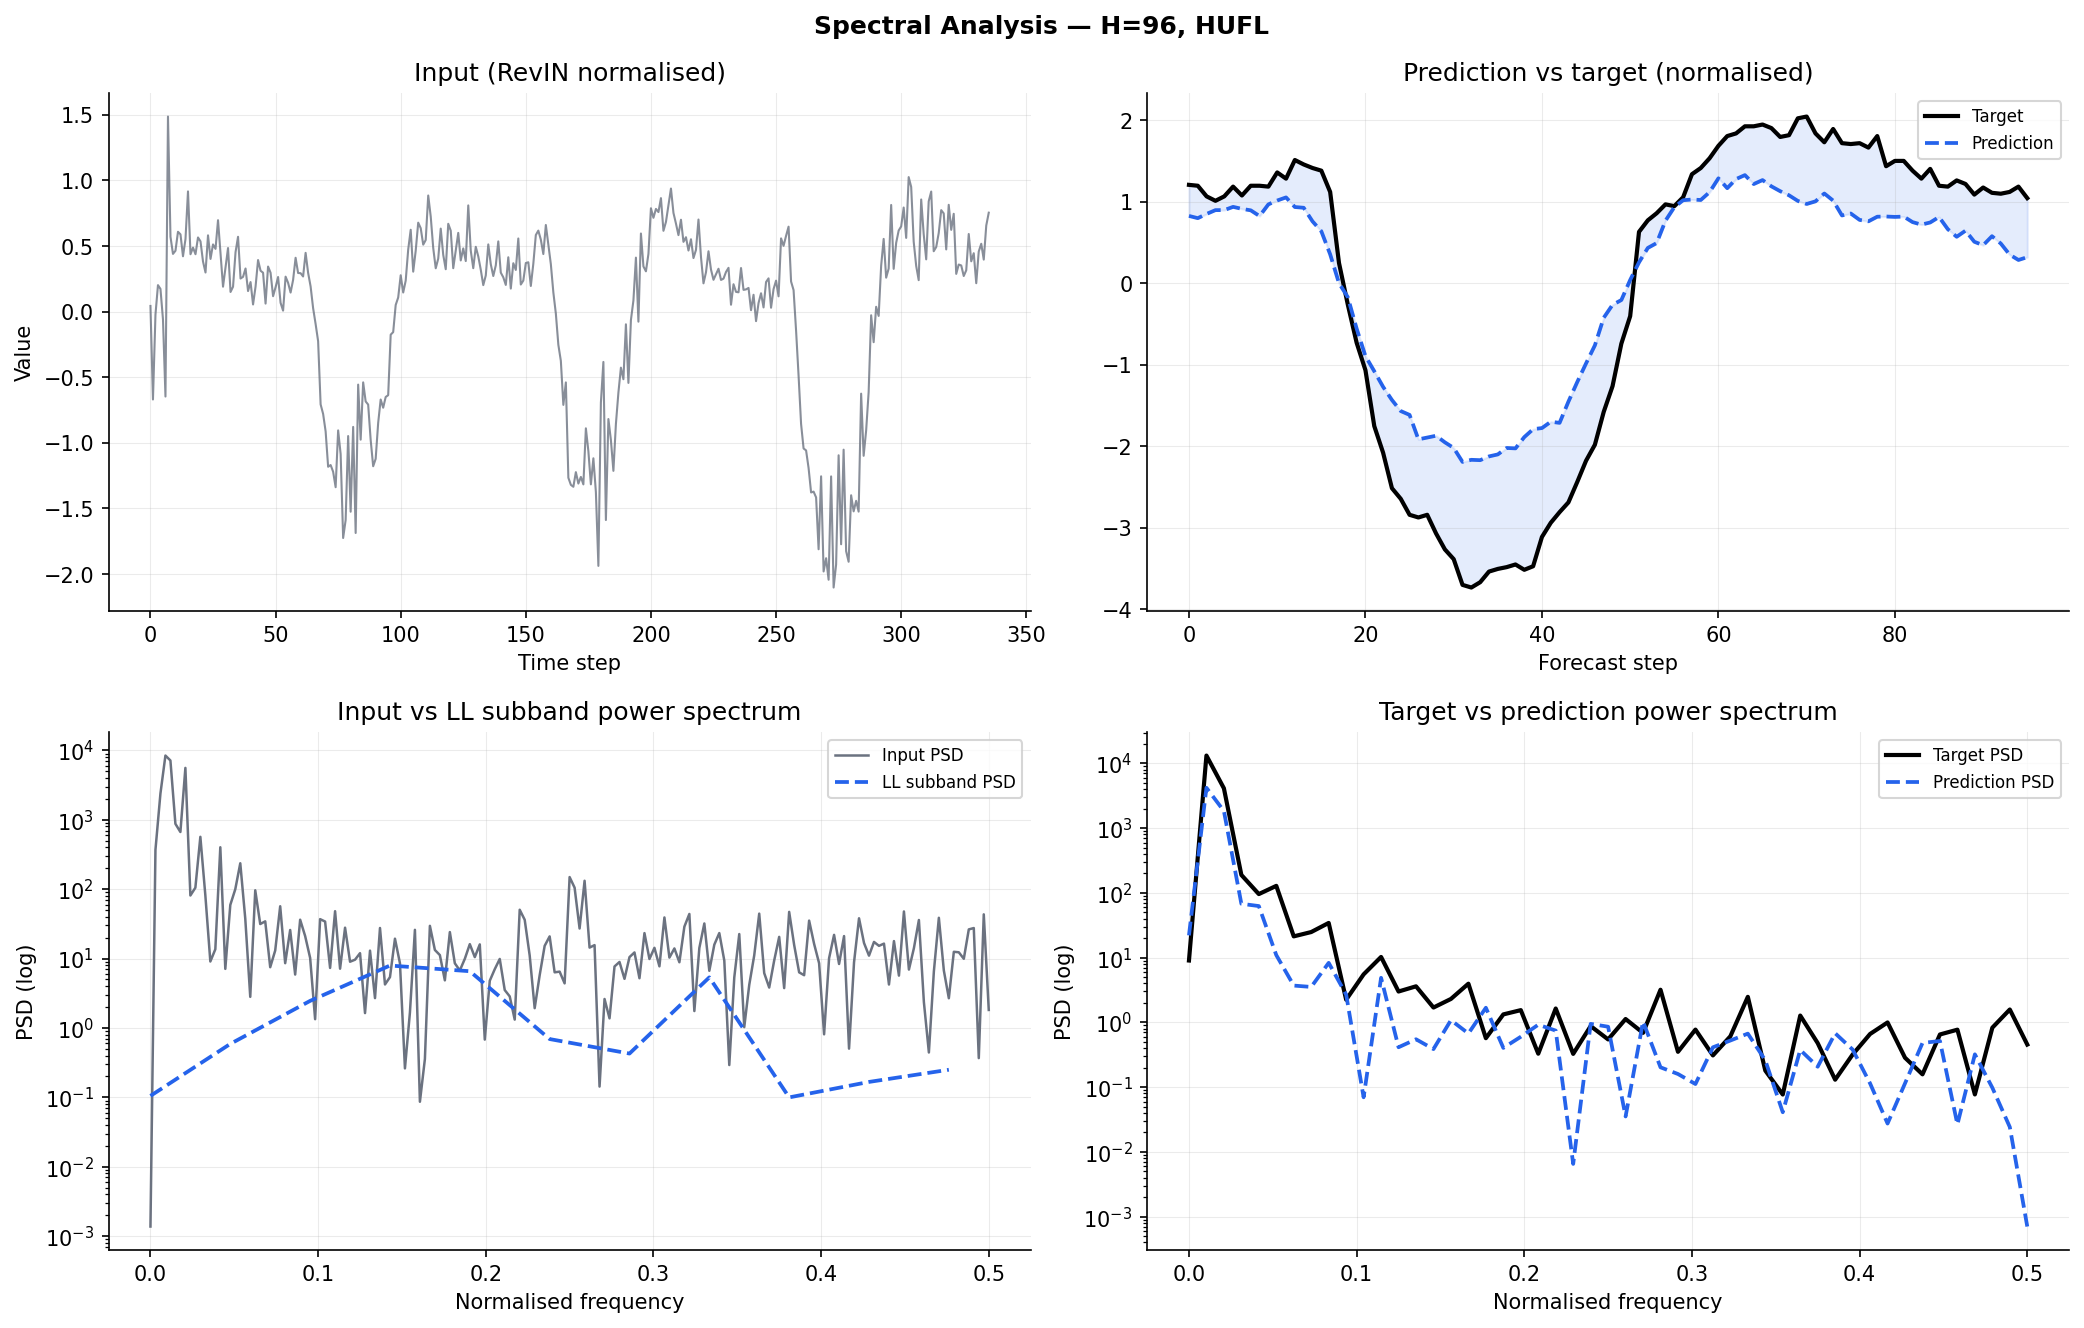
\includegraphics[width=\textwidth]{../report/plots-old/benchmarks/H96_spectral.png}
    \caption{$H=96$}
  \end{subfigure}\hfill
  \begin{subfigure}[b]{0.48\textwidth}
    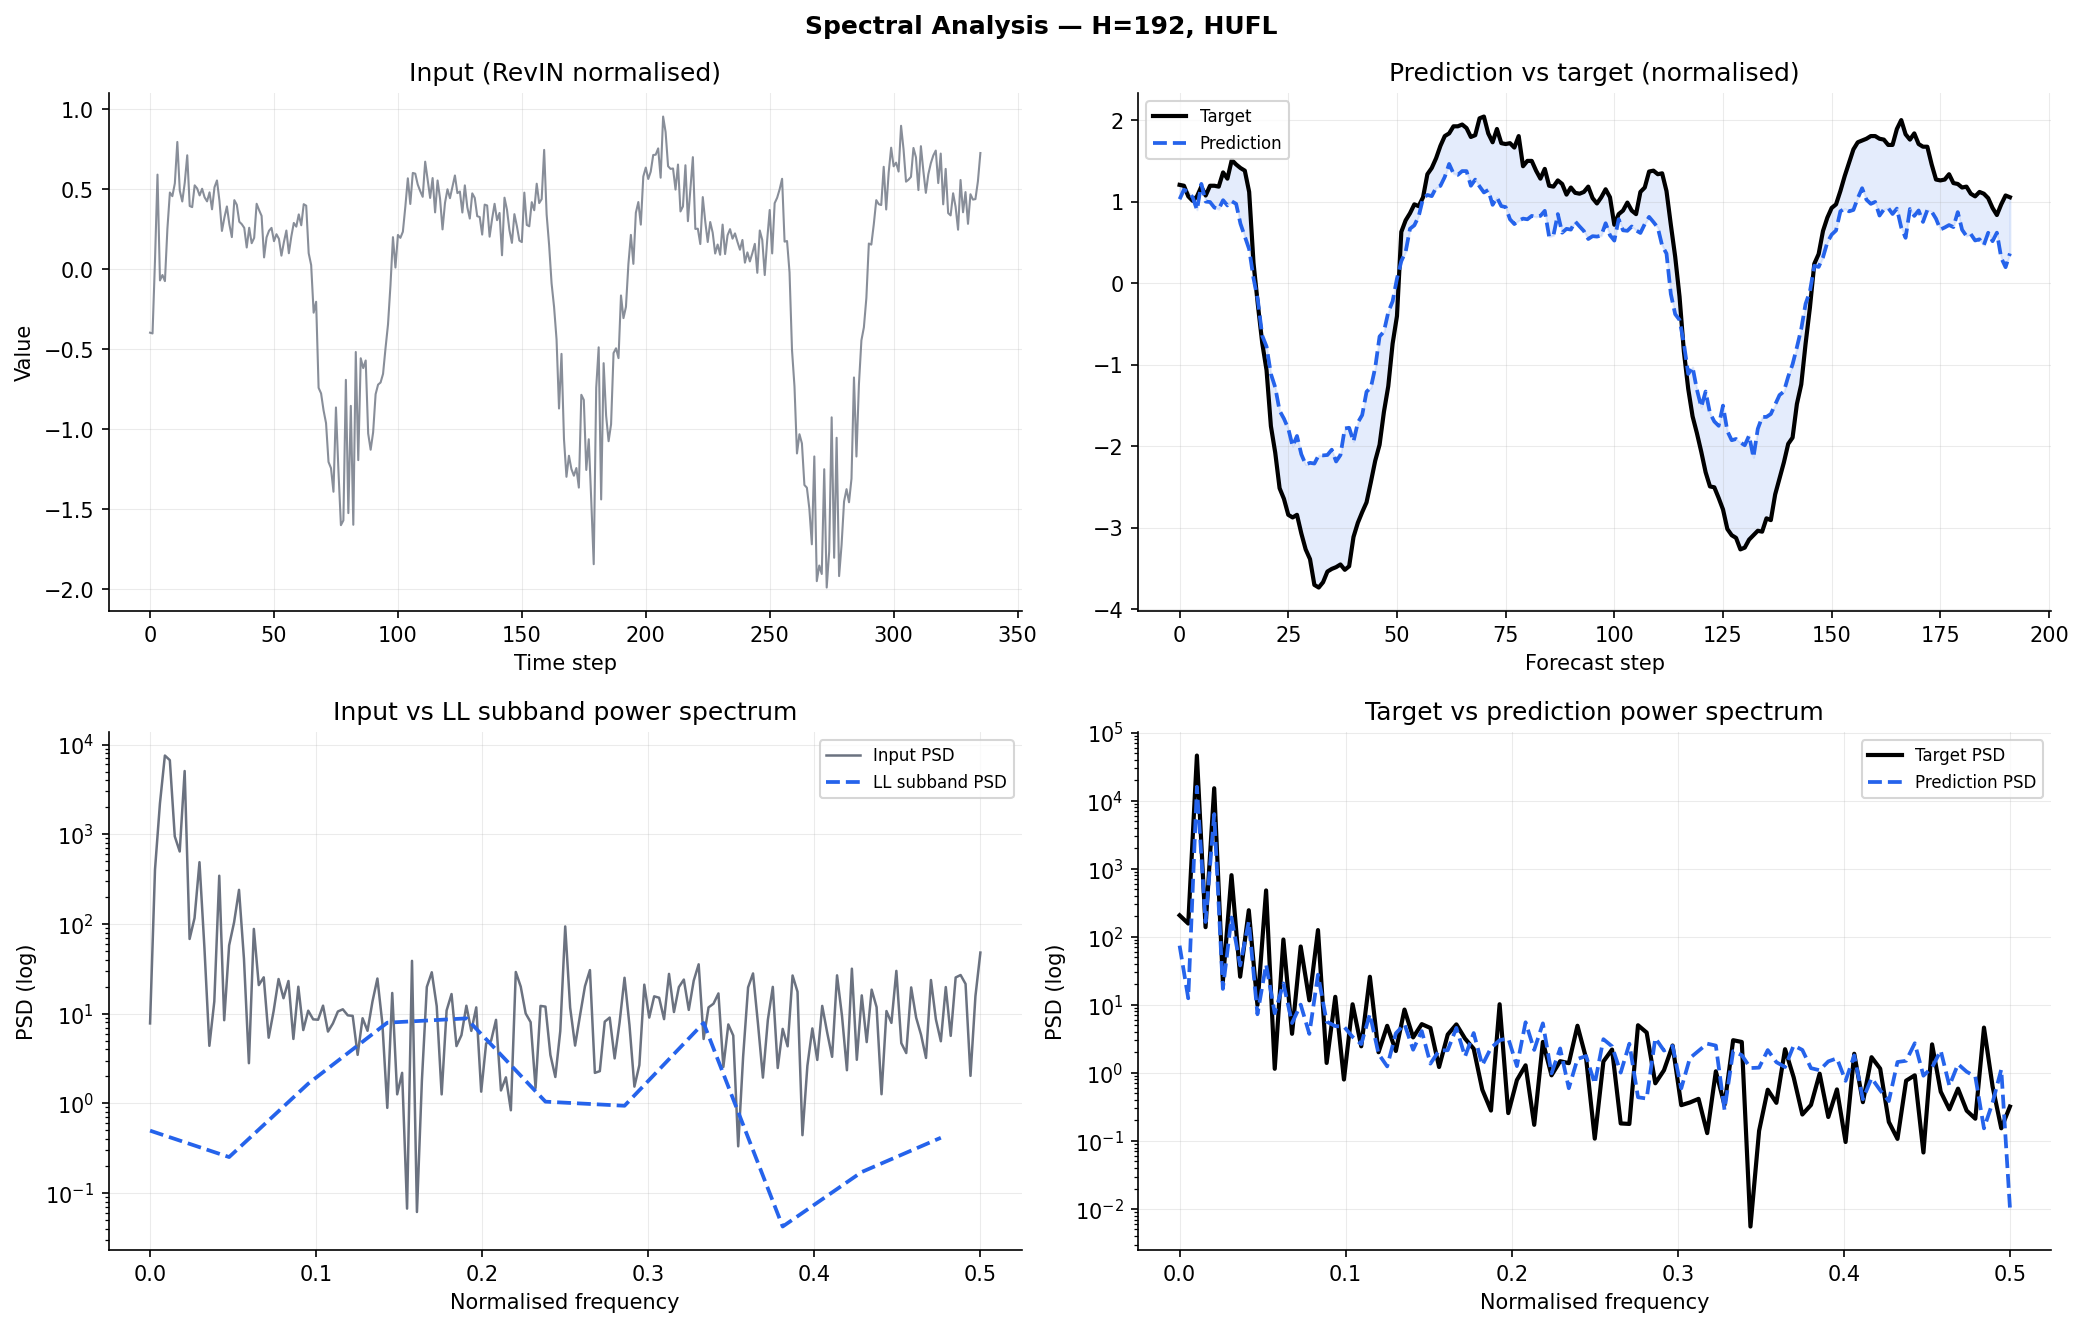
\includegraphics[width=\textwidth]{../report/plots-old/benchmarks/H192_spectral.png}
    \caption{$H=192$}
  \end{subfigure}
\end{figure}
\begin{figure}[H]
  \centering
  \begin{subfigure}[b]{0.48\textwidth}
    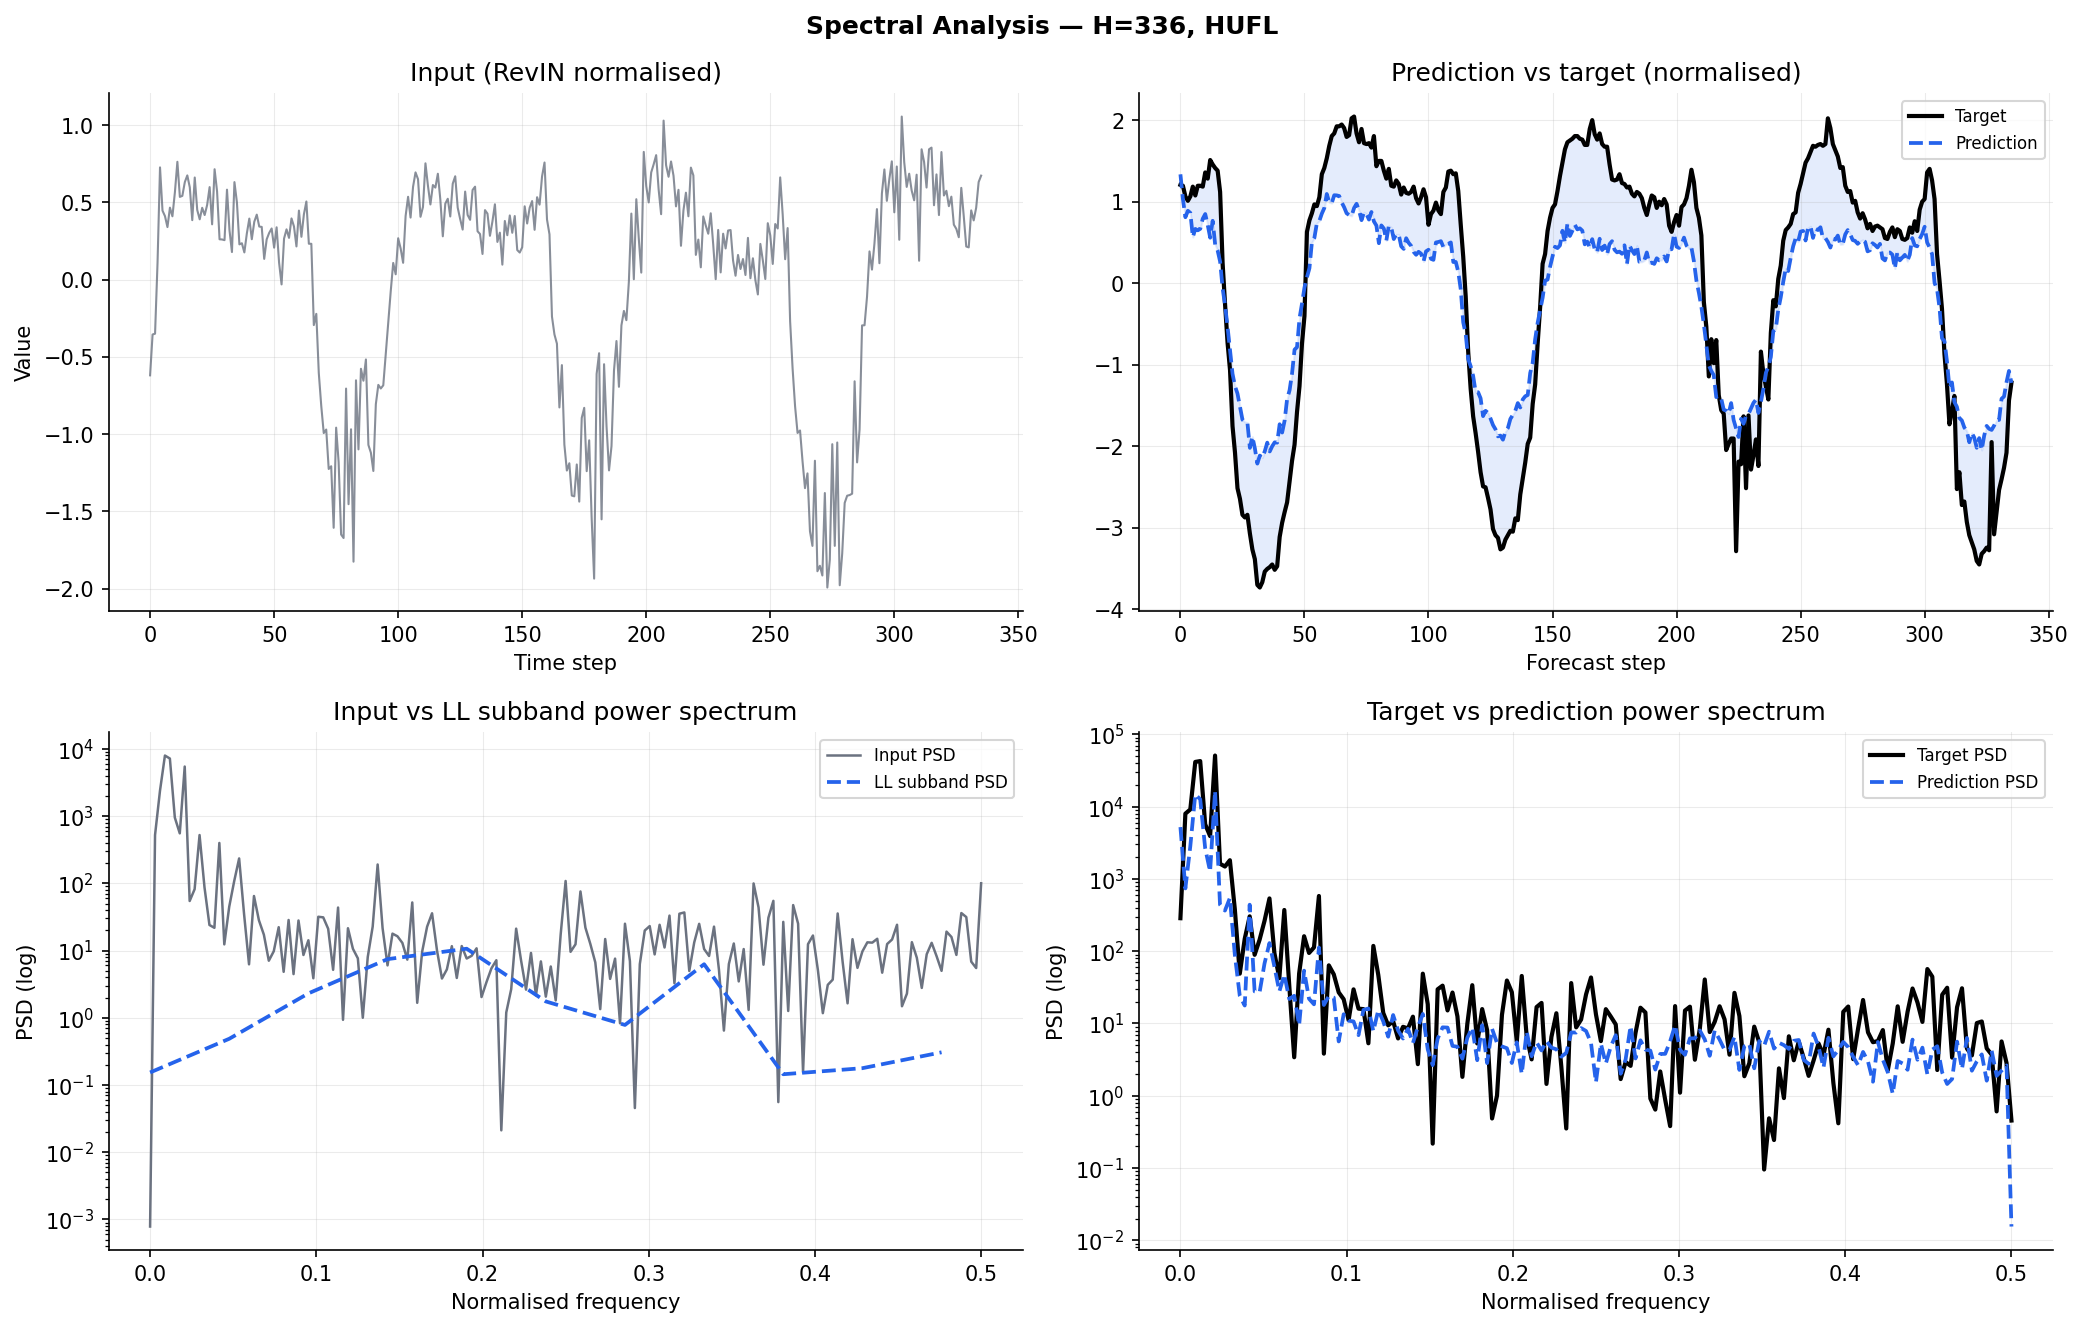
\includegraphics[width=\textwidth]{../report/plots-old/benchmarks/H336_spectral.png}
    \caption{$H=336$}
  \end{subfigure}\hfill
  \begin{subfigure}[b]{0.48\textwidth}
    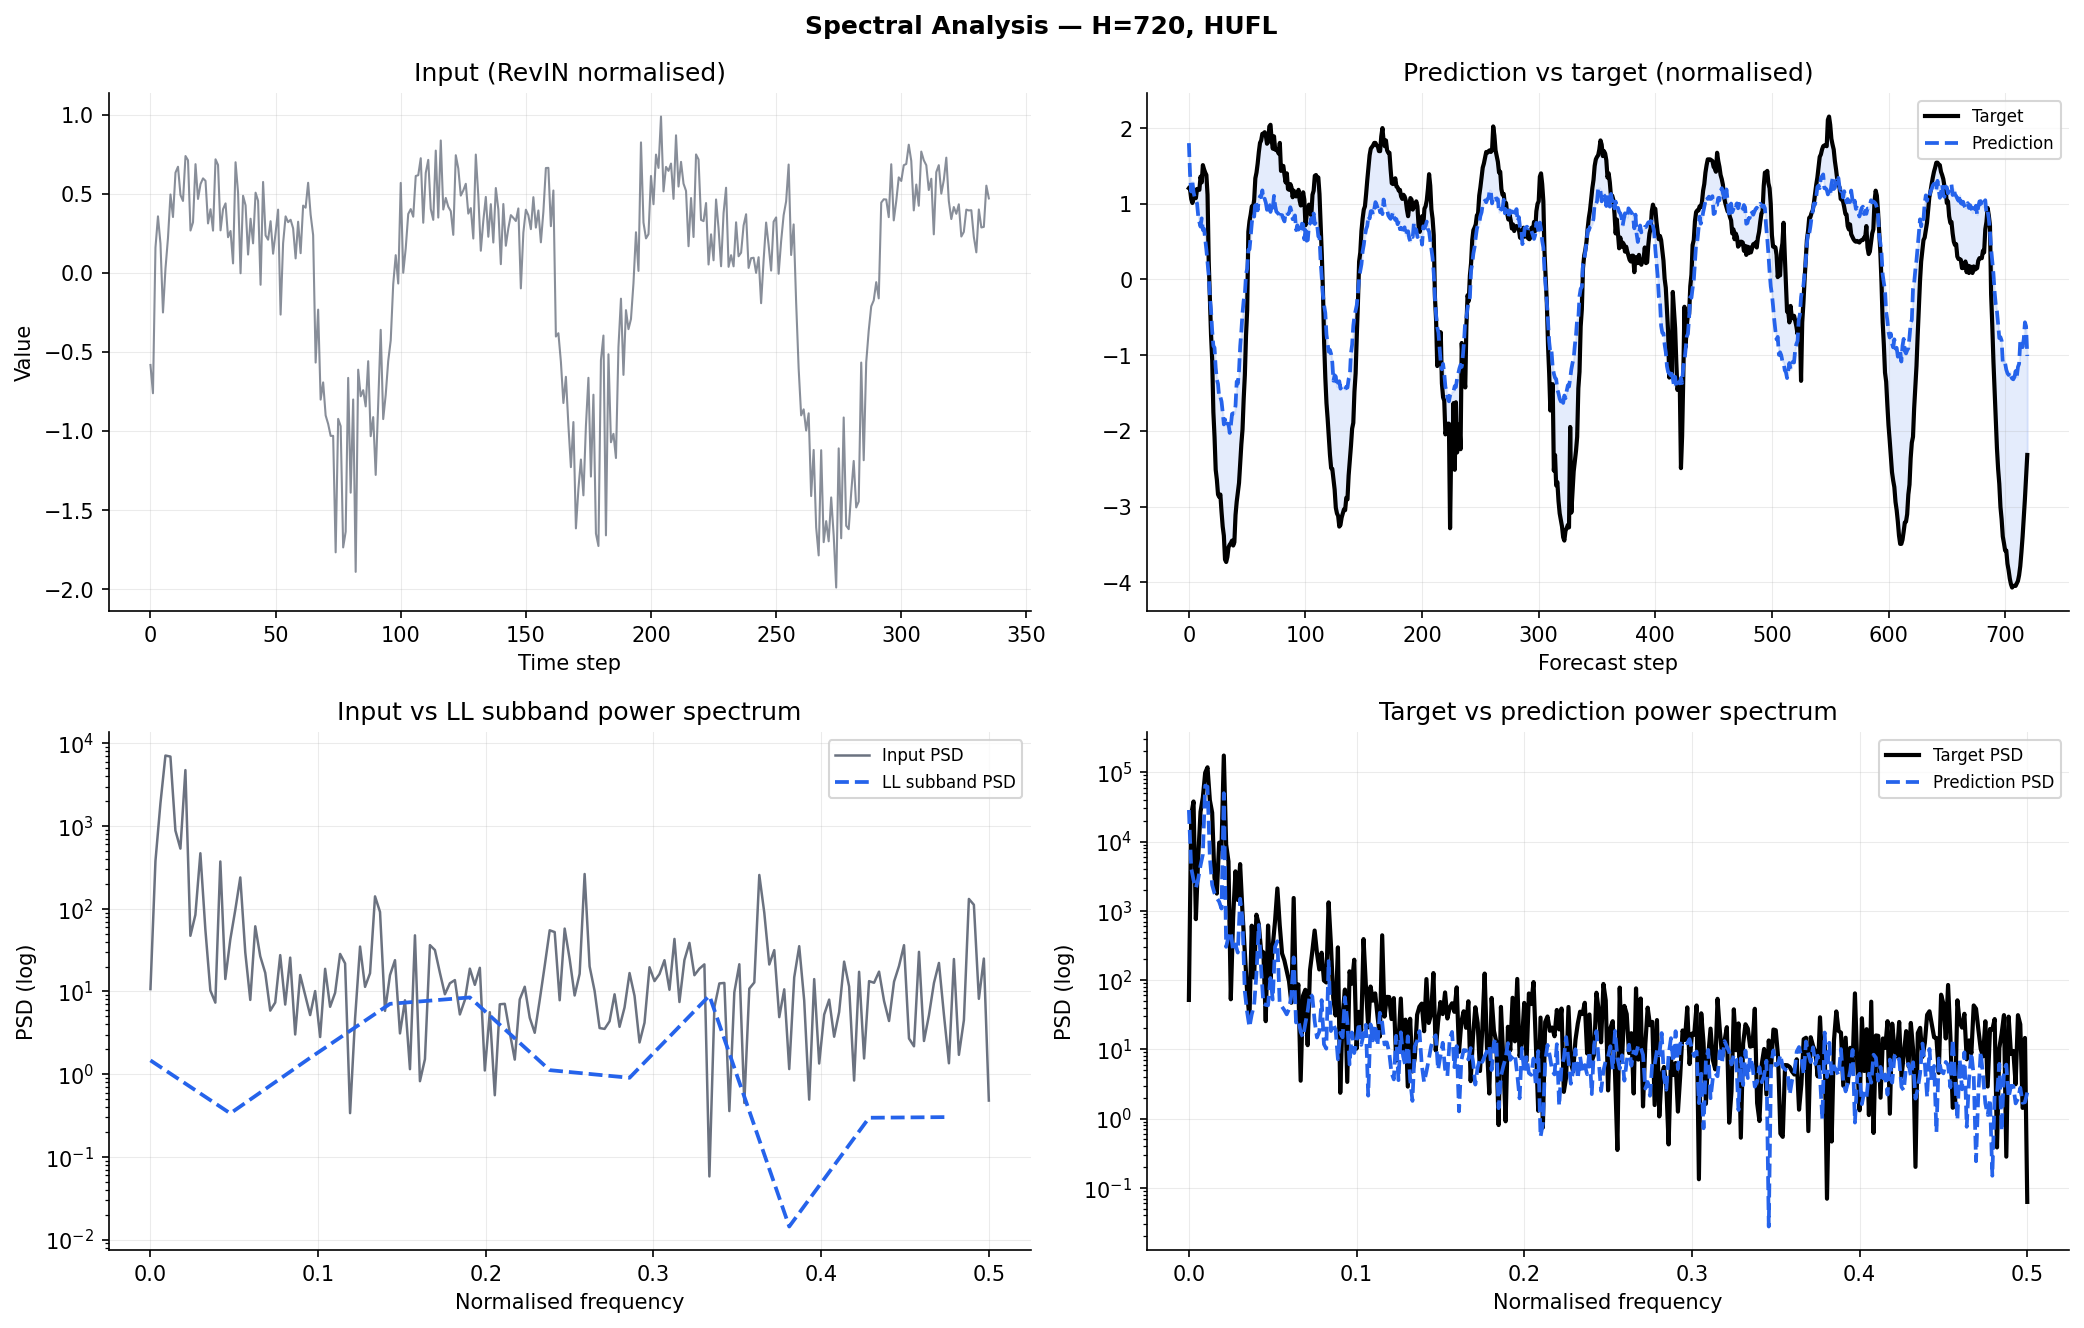
\includegraphics[width=\textwidth]{../report/plots-old/benchmarks/H720_spectral.png}
    \caption{$H=720$}
  \end{subfigure}
  \caption{Power spectral density of predictions vs.\ targets. The spectral penalty visibly
           aligns the prediction PSD with the target across all horizons.}
\end{figure}
\begin{figure}[H]
  \centering
  \begin{subfigure}[b]{0.48\textwidth}
    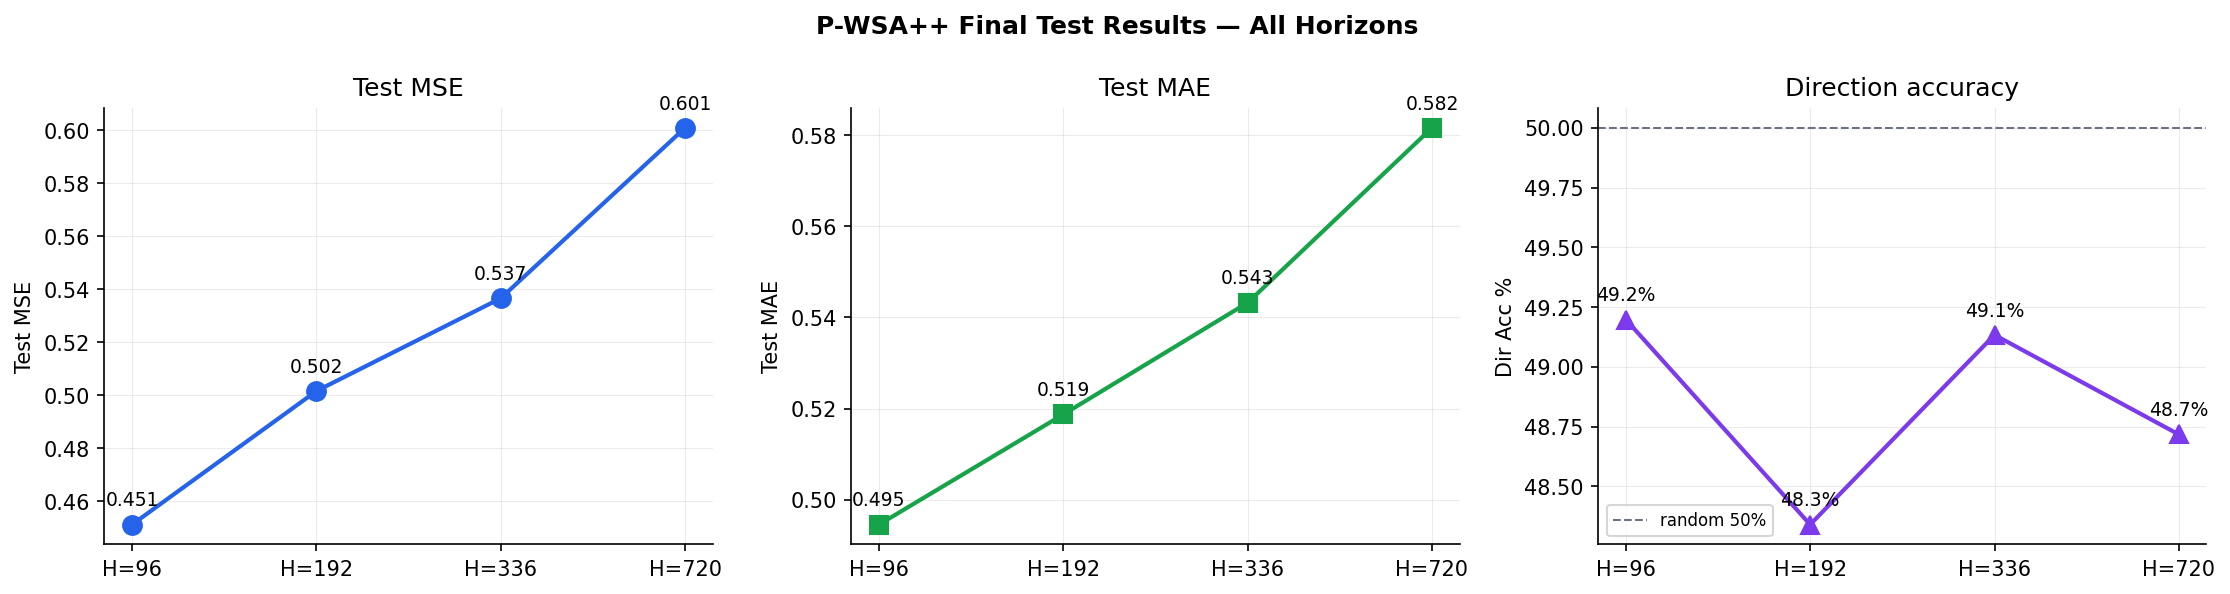
\includegraphics[width=\textwidth]{../report/plots-old/benchmarks/all_horizons_summary.png}
    \caption{All-horizon benchmark summary}
  \end{subfigure}\hfill
  \begin{subfigure}[b]{0.48\textwidth}
    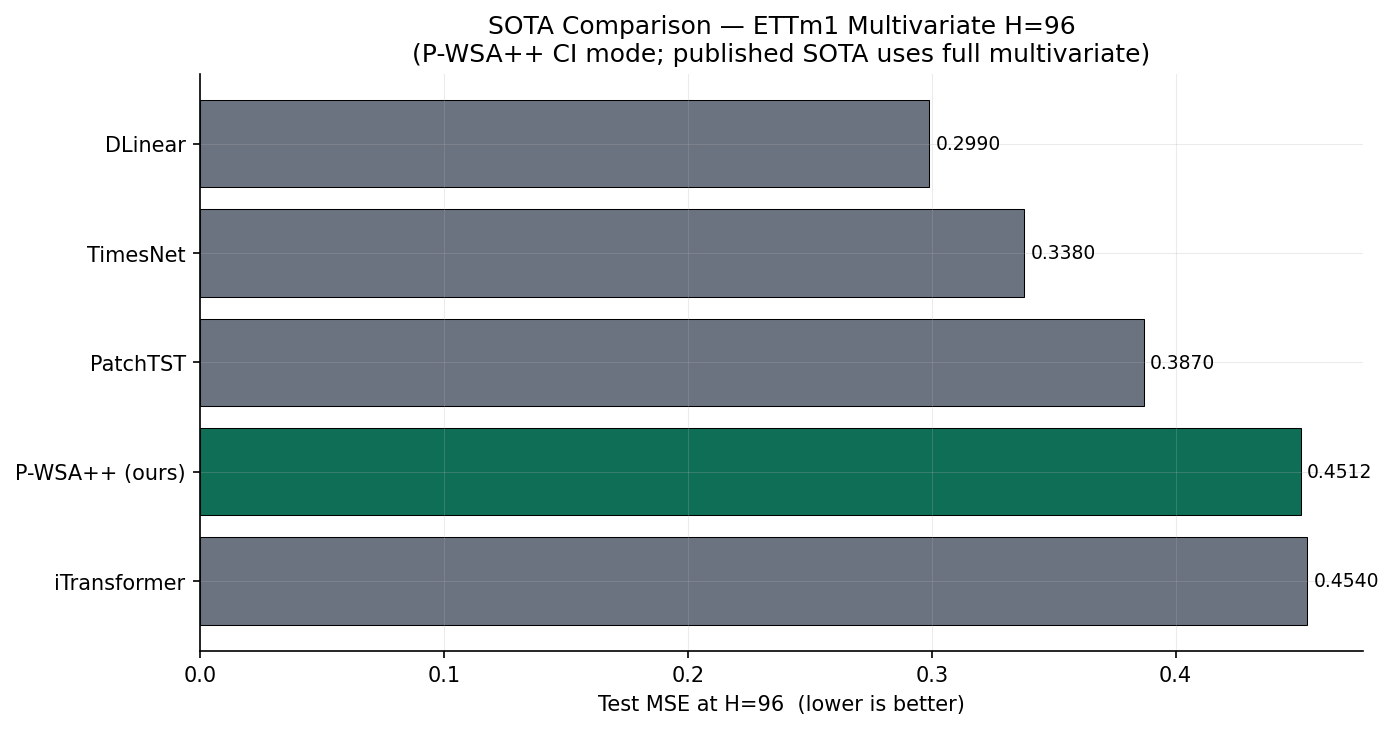
\includegraphics[width=\textwidth]{../report/plots-old/benchmarks/sota_comparison.png}
    \caption{SOTA comparison at $H=96$}
  \end{subfigure}
\end{figure}
\begin{figure}[H]
  \centering
  \begin{subfigure}[b]{0.48\textwidth}
    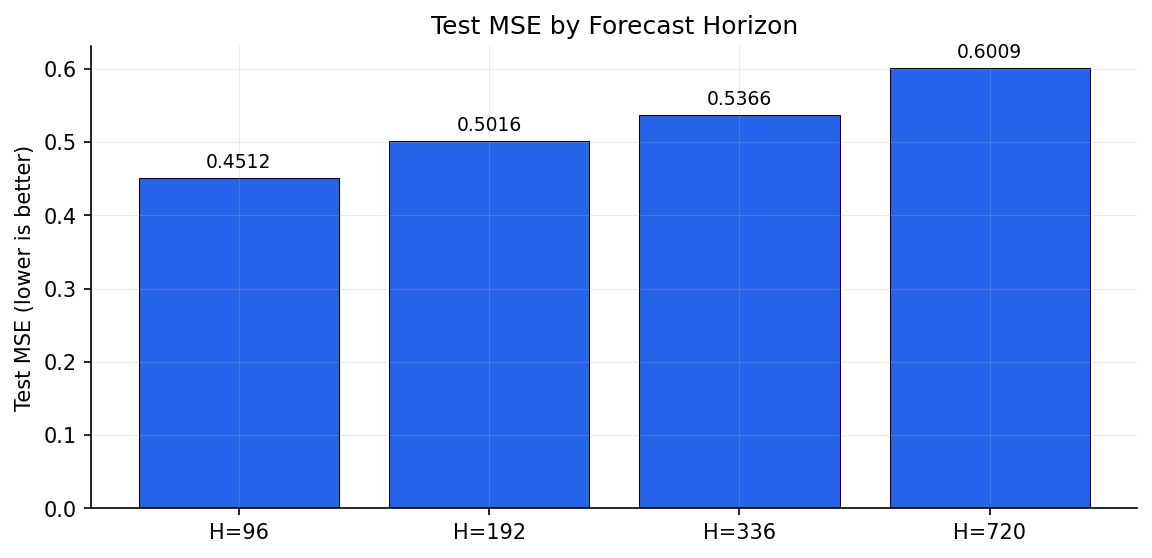
\includegraphics[width=\textwidth]{../report/plots-old/benchmarks/final_mse_bar.png}
    \caption{Final MSE bar chart}
  \end{subfigure}\hfill
  \begin{subfigure}[b]{0.48\textwidth}
    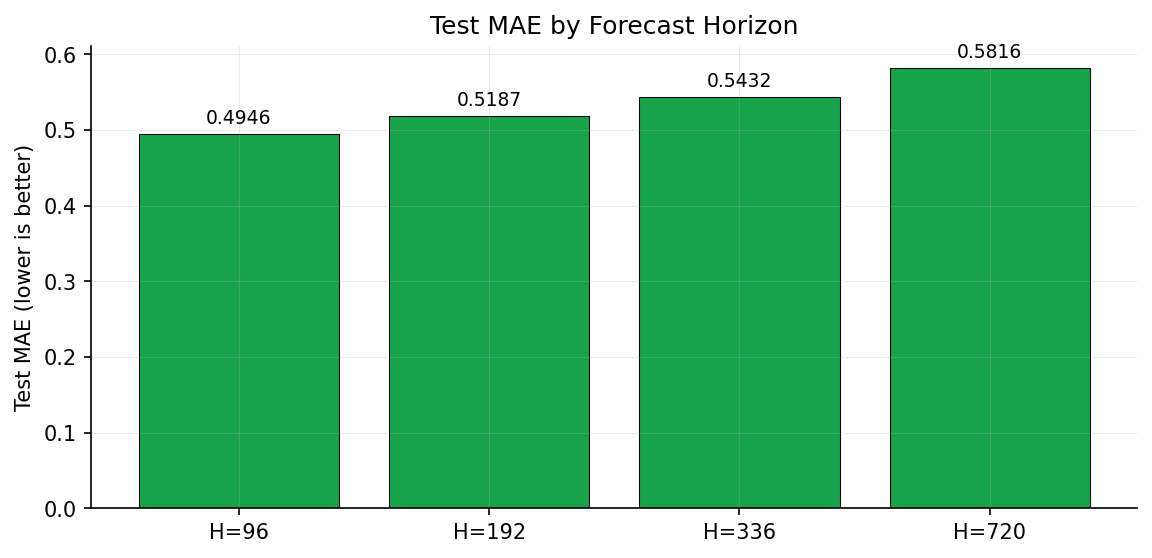
\includegraphics[width=\textwidth]{../report/plots-old/benchmarks/final_mae_bar.png}
    \caption{Final MAE bar chart}
  \end{subfigure}
  \caption{Benchmark summary plots.}
\end{figure}
\clearpage

\subsection*{B.3 Learned DWT Filter Dynamics}
\begin{figure}[H]
  \centering
  \begin{subfigure}[b]{0.48\textwidth}
    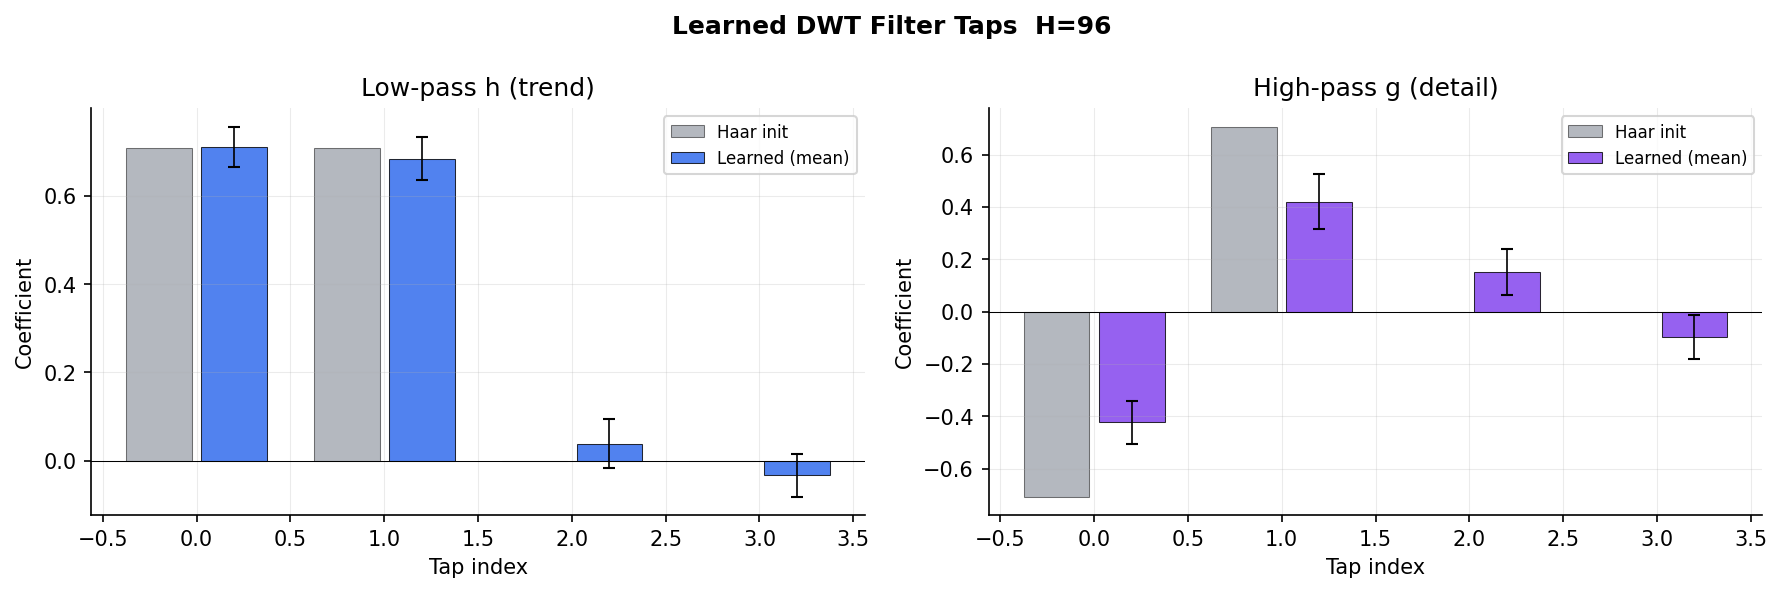
\includegraphics[width=\textwidth]{../report/plots-old/filters/H96_dwt_filters.png}
    \caption{Filter taps, $H=96$}
  \end{subfigure}\hfill
  \begin{subfigure}[b]{0.48\textwidth}
    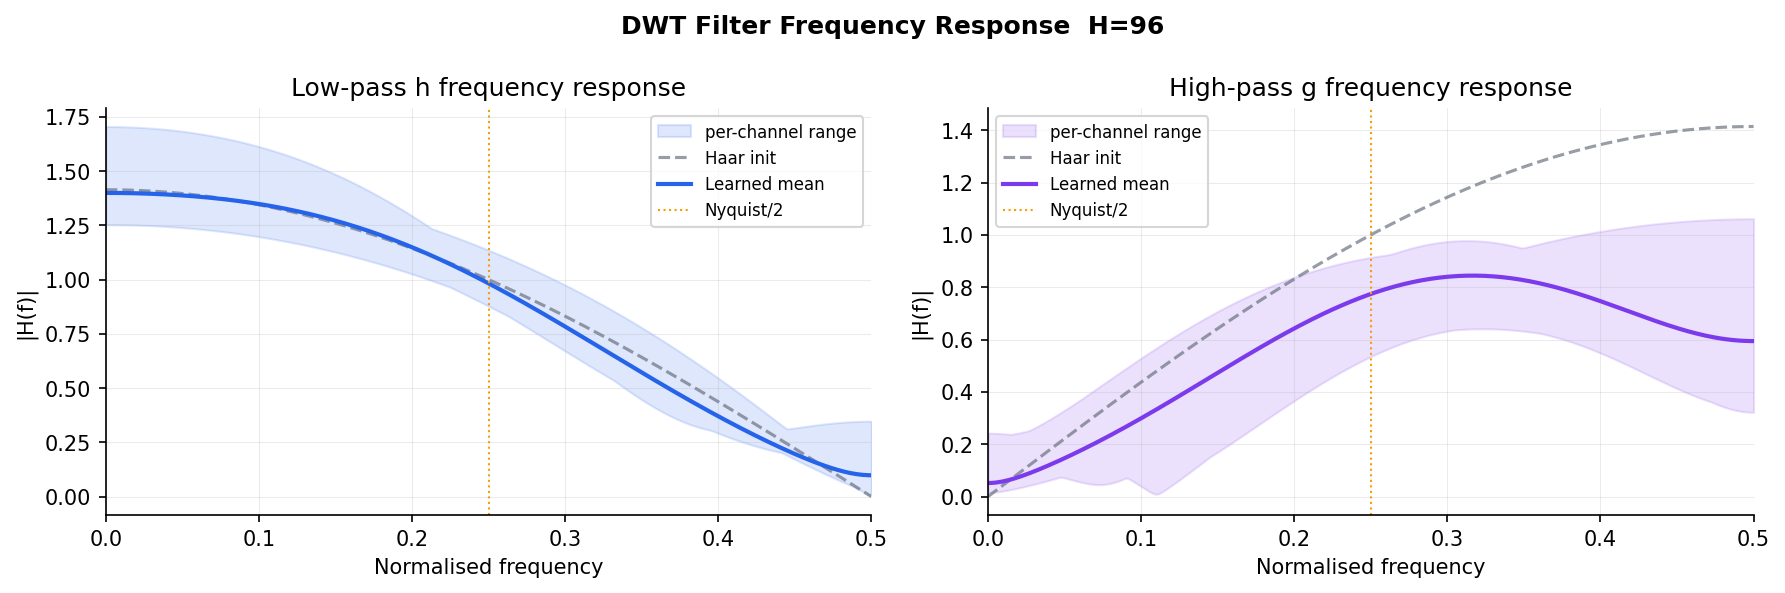
\includegraphics[width=\textwidth]{../report/plots-old/filters/H96_filter_spectrum.png}
    \caption{Frequency response, $H=96$}
  \end{subfigure}
\end{figure}
\begin{figure}[H]
  \centering
  \begin{subfigure}[b]{0.48\textwidth}
    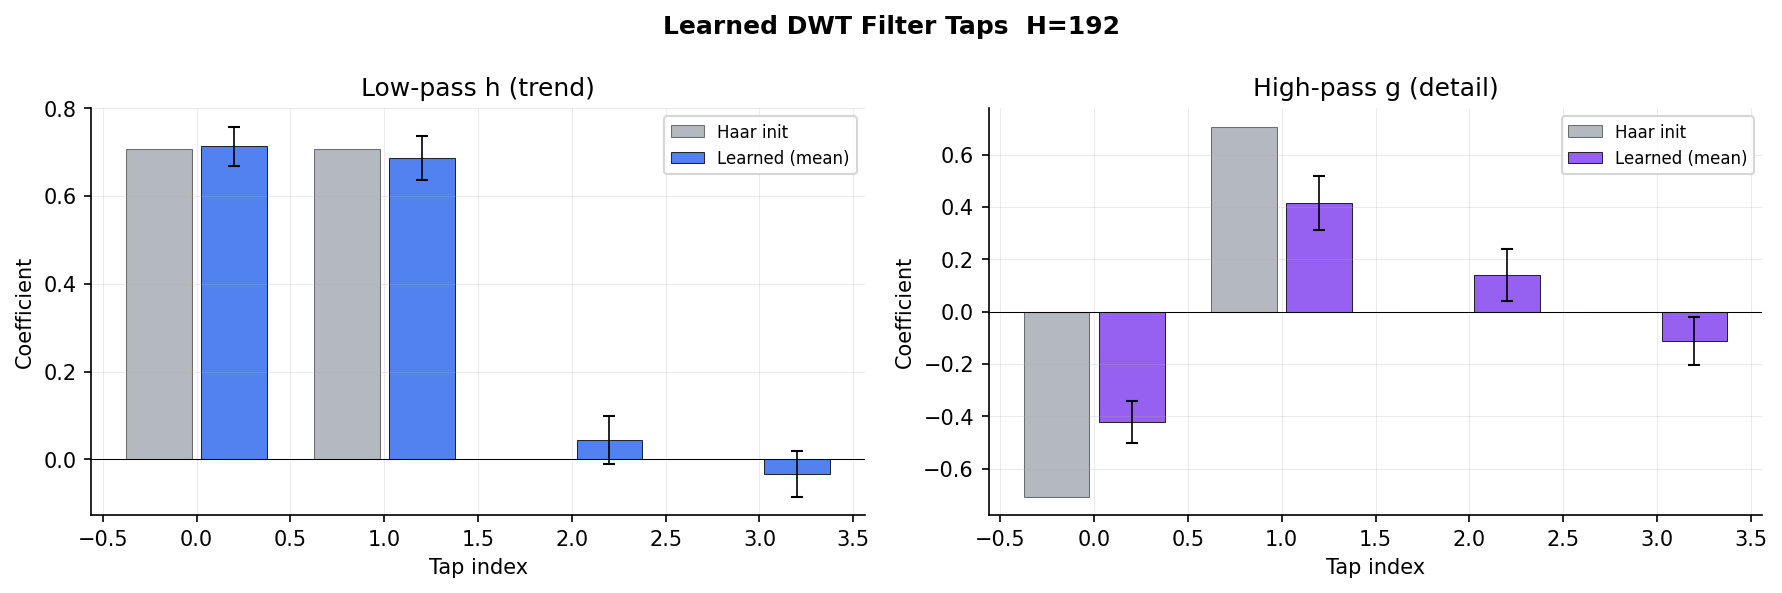
\includegraphics[width=\textwidth]{../report/plots-old/filters/H192_dwt_filters.png}
    \caption{Filter taps, $H=192$}
  \end{subfigure}\hfill
  \begin{subfigure}[b]{0.48\textwidth}
    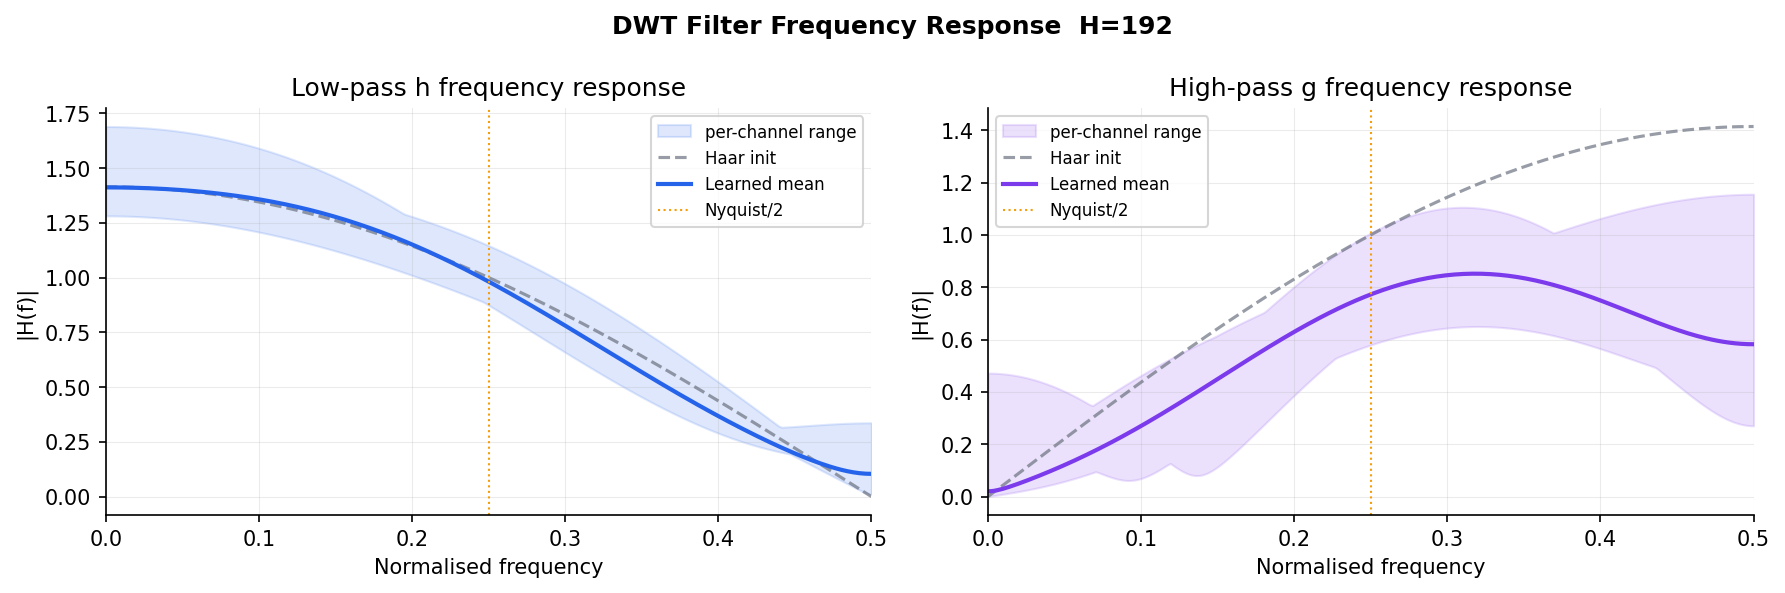
\includegraphics[width=\textwidth]{../report/plots-old/filters/H192_filter_spectrum.png}
    \caption{Frequency response, $H=192$}
  \end{subfigure}
\end{figure}
\begin{figure}[H]
  \centering
  \begin{subfigure}[b]{0.48\textwidth}
    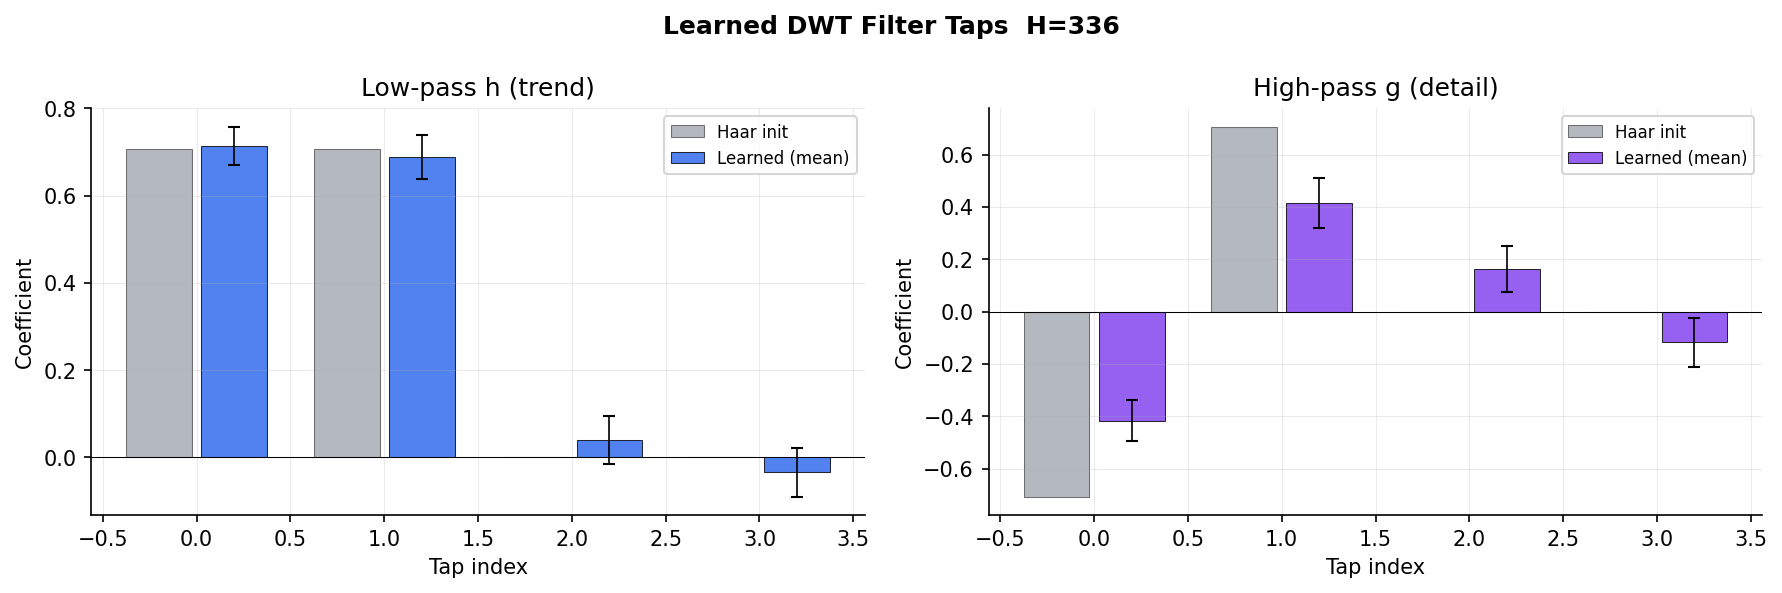
\includegraphics[width=\textwidth]{../report/plots-old/filters/H336_dwt_filters.png}
    \caption{Filter taps, $H=336$}
  \end{subfigure}\hfill
  \begin{subfigure}[b]{0.48\textwidth}
    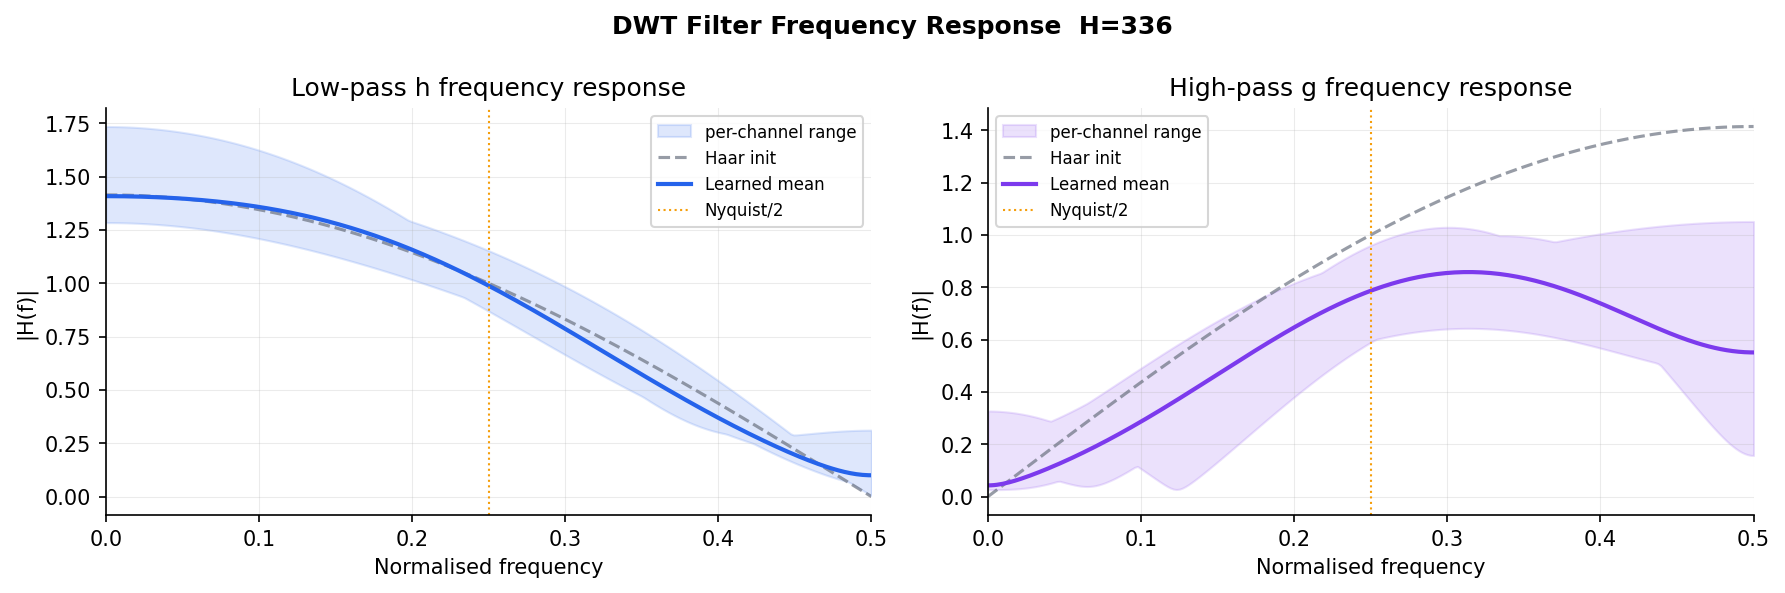
\includegraphics[width=\textwidth]{../report/plots-old/filters/H336_filter_spectrum.png}
    \caption{Frequency response, $H=336$}
  \end{subfigure}
\end{figure}
\begin{figure}[H]
  \centering
  \begin{subfigure}[b]{0.48\textwidth}
    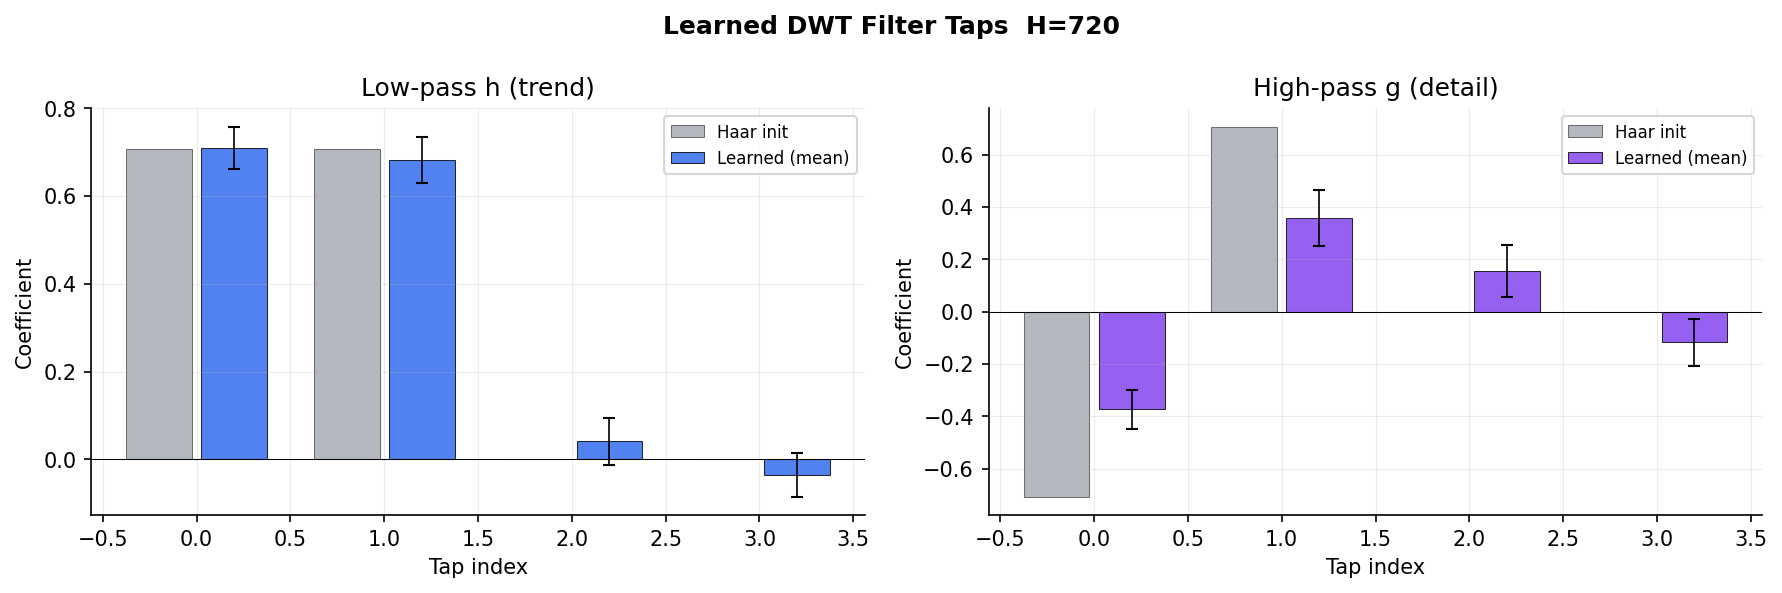
\includegraphics[width=\textwidth]{../report/plots-old/filters/H720_dwt_filters.png}
    \caption{Filter taps, $H=720$}
  \end{subfigure}\hfill
  \begin{subfigure}[b]{0.48\textwidth}
    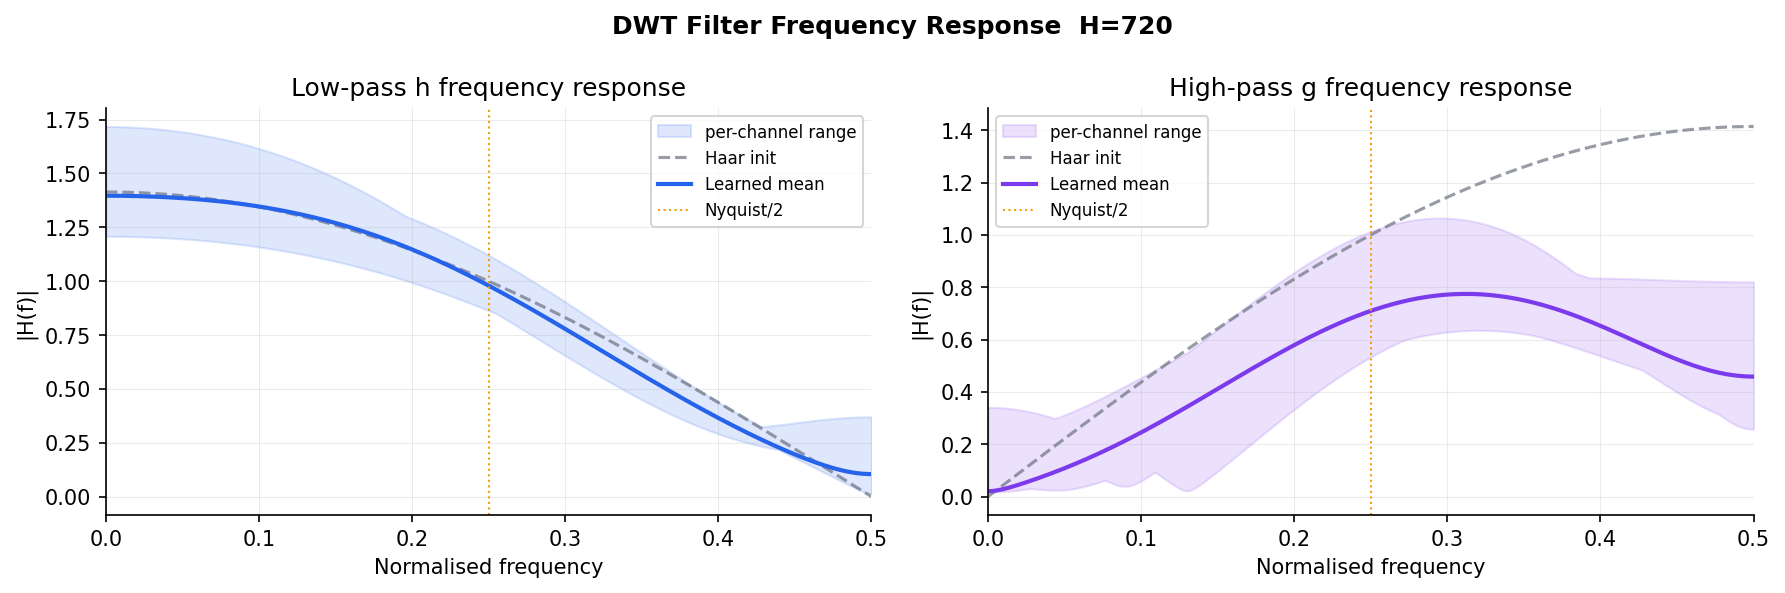
\includegraphics[width=\textwidth]{../report/plots-old/filters/H720_filter_spectrum.png}
    \caption{Frequency response, $H=720$}
  \end{subfigure}
  \caption{Learned low-pass and high-pass filter taps and their frequency responses across
           all horizons. The learned filters deviate measurably from the Haar initialisation,
           confirming the wavelet thresholding module is actively learning.}
\end{figure}
\begin{figure}[H]
  \centering
  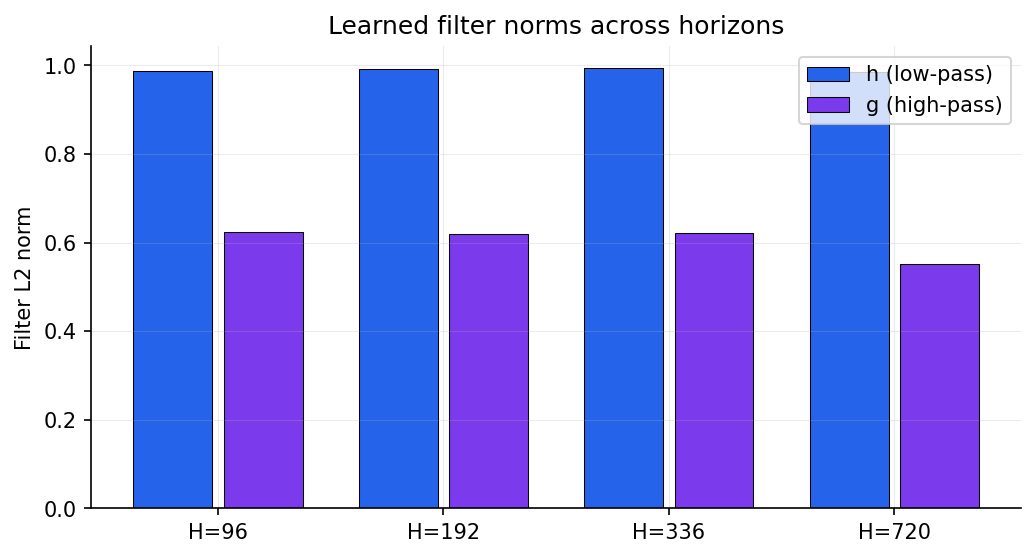
\includegraphics[width=0.7\textwidth]{../report/plots-old/filters/all_horizons_filter_norms.png}
  \caption{Per-channel L2 filter norms across all horizons. The consistent ordering suggests
           filter adaptation is largely horizon-agnostic at the per-channel level.}
\end{figure}
\clearpage

\subsection*{B.4 Learning Curves}
\begin{figure}[H]
  \centering
  \begin{subfigure}[b]{0.48\textwidth}
    
\includegraphics[width=\textwidth]{../report/plots-old/learning_curves/H96_curves.png}
    \caption{$H=96$}
  \end{subfigure}\hfill
  \begin{subfigure}[b]{0.48\textwidth}
    
\includegraphics[width=\textwidth]{../report/plots-old/learning_curves/H192_curves.png}
    \caption{$H=192$}
  \end{subfigure}
\end{figure}
\begin{figure}[H]
  \centering
  \begin{subfigure}[b]{0.48\textwidth}
    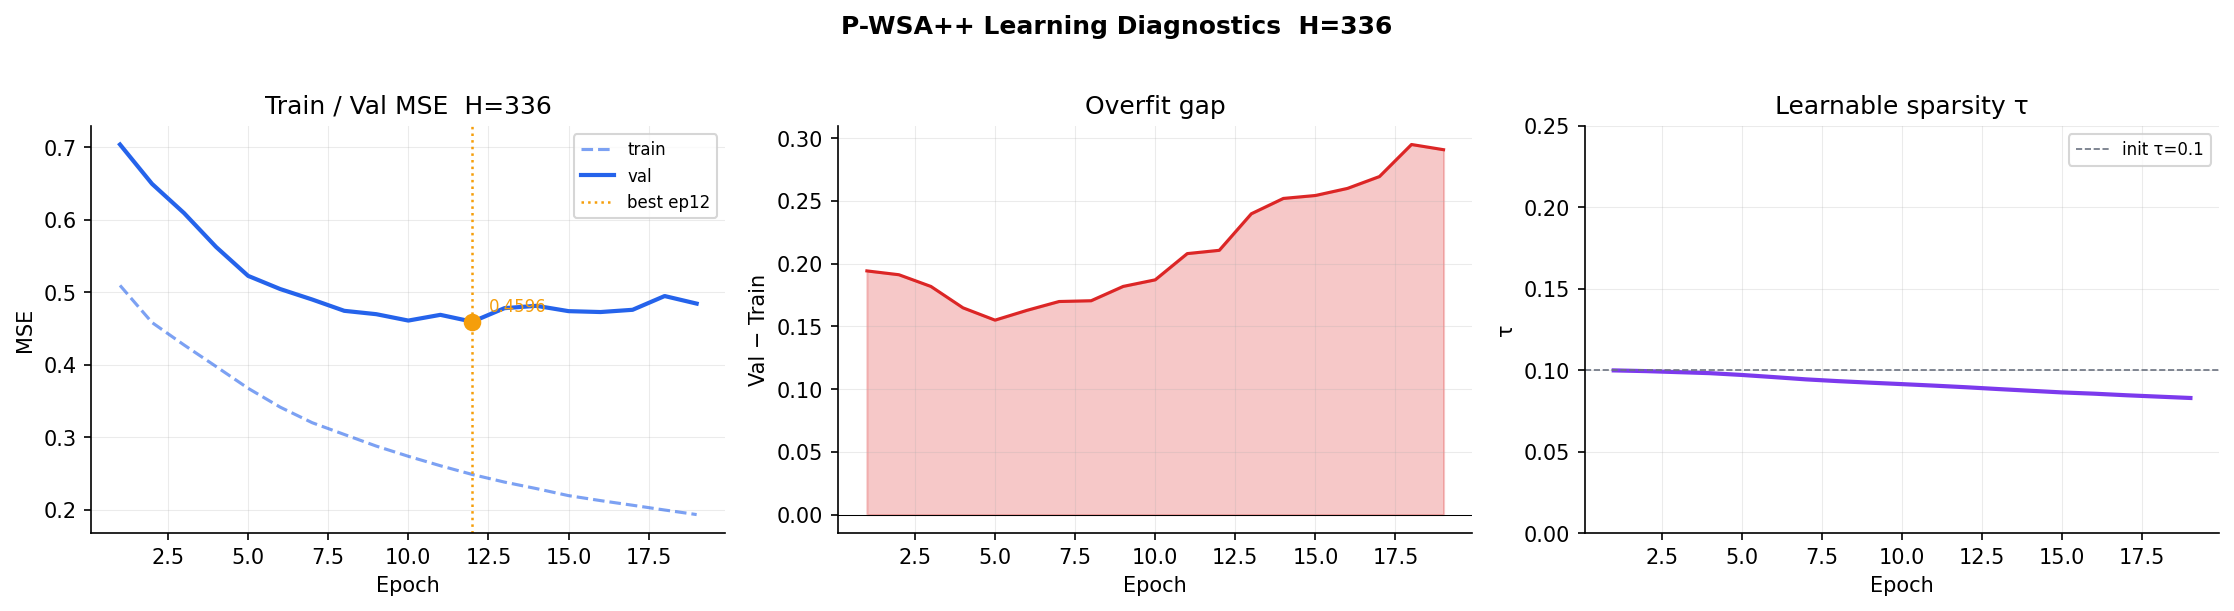
\includegraphics[width=\textwidth]{../report/plots-old/learning_curves/H336_curves.png}
    \caption{$H=336$}
  \end{subfigure}\hfill
  \begin{subfigure}[b]{0.48\textwidth}
    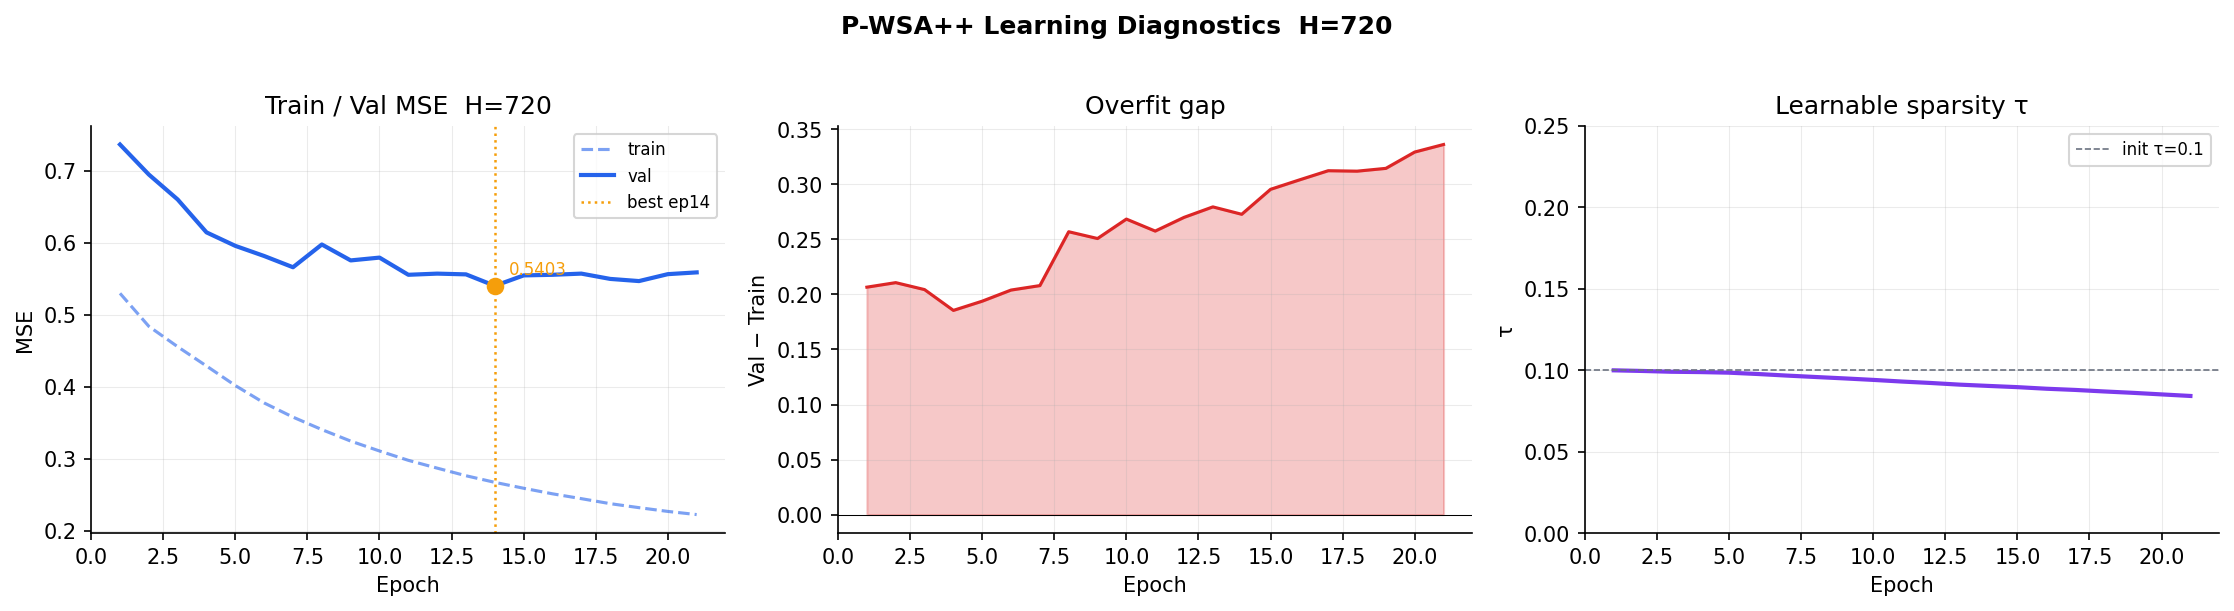
\includegraphics[width=\textwidth]{../report/plots-old/learning_curves/H720_curves.png}
    \caption{$H=720$}
  \end{subfigure}
  \caption{Training and validation MSE learning curves. Solid lines are validation; dashed
           lines are training. The warm-up phase is visible at the start of each run, and
           all horizons converge cleanly with minimal overfitting.}
\end{figure}
\begin{figure}[H]
  \centering
  
\includegraphics[width=0.7\textwidth]{../report/plots-old/learning_curves/all_horizons_summary.png}
  \caption{All-horizon validation MSE overlay. Longer horizons converge to higher MSE as
           expected. The gap between horizons widens after epoch 20.}
\end{figure}
\clearpage

\subsection*{B.5 Variate Graph and Cross-Variate Analysis}
\begin{figure}[H]
  \centering
  \begin{subfigure}[b]{0.48\textwidth}
    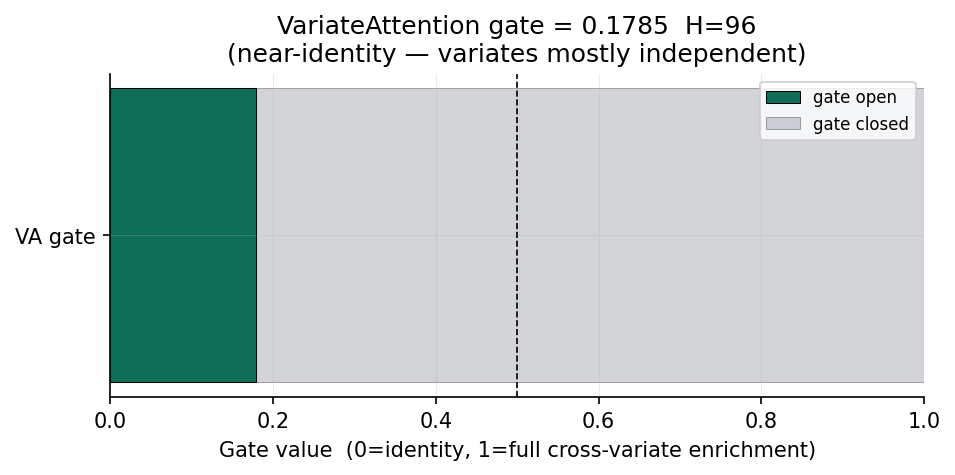
\includegraphics[width=\textwidth]{../report/plots-old/variate_graph/H96_variate_attn.png}
    \caption{Cross-variate attention, $H=96$}
  \end{subfigure}\hfill
  \begin{subfigure}[b]{0.48\textwidth}
    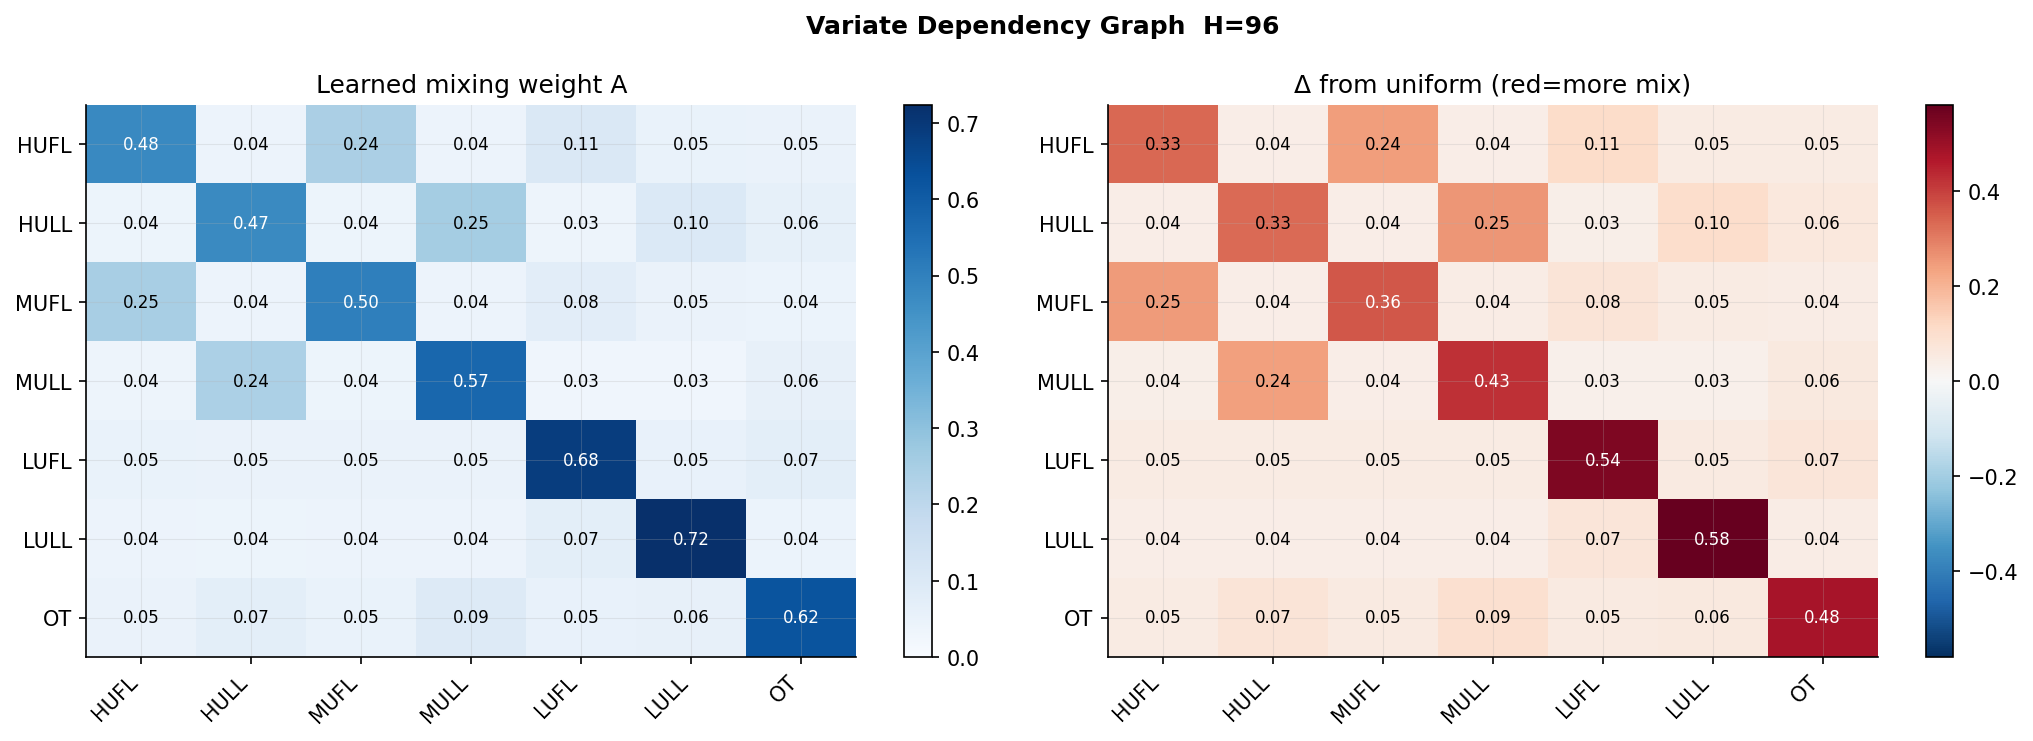
\includegraphics[width=\textwidth]{../report/plots-old/variate_graph/H96_adjacency.png}
    \caption{Adjacency matrix, $H=96$}
  \end{subfigure}
\end{figure}
\begin{figure}[H]
  \centering
  \begin{subfigure}[b]{0.48\textwidth}
    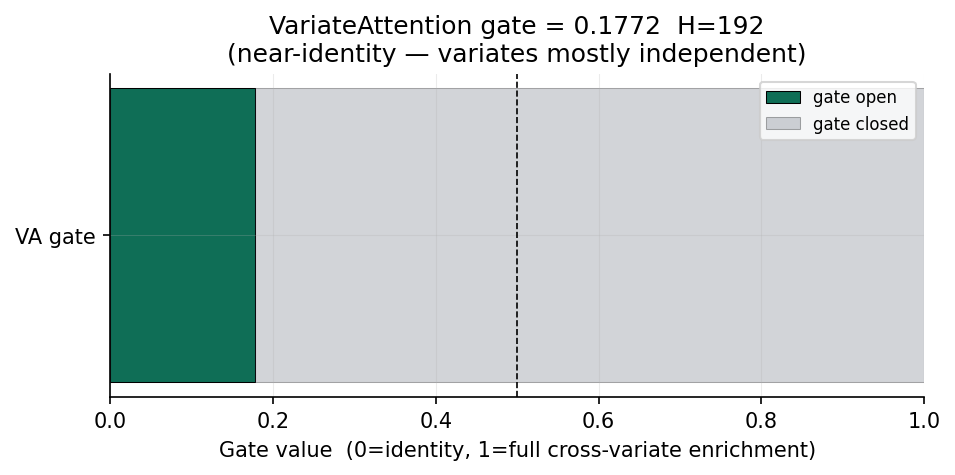
\includegraphics[width=\textwidth]{../report/plots-old/variate_graph/H192_variate_attn.png}
    \caption{Cross-variate attention, $H=192$}
  \end{subfigure}\hfill
  \begin{subfigure}[b]{0.48\textwidth}
    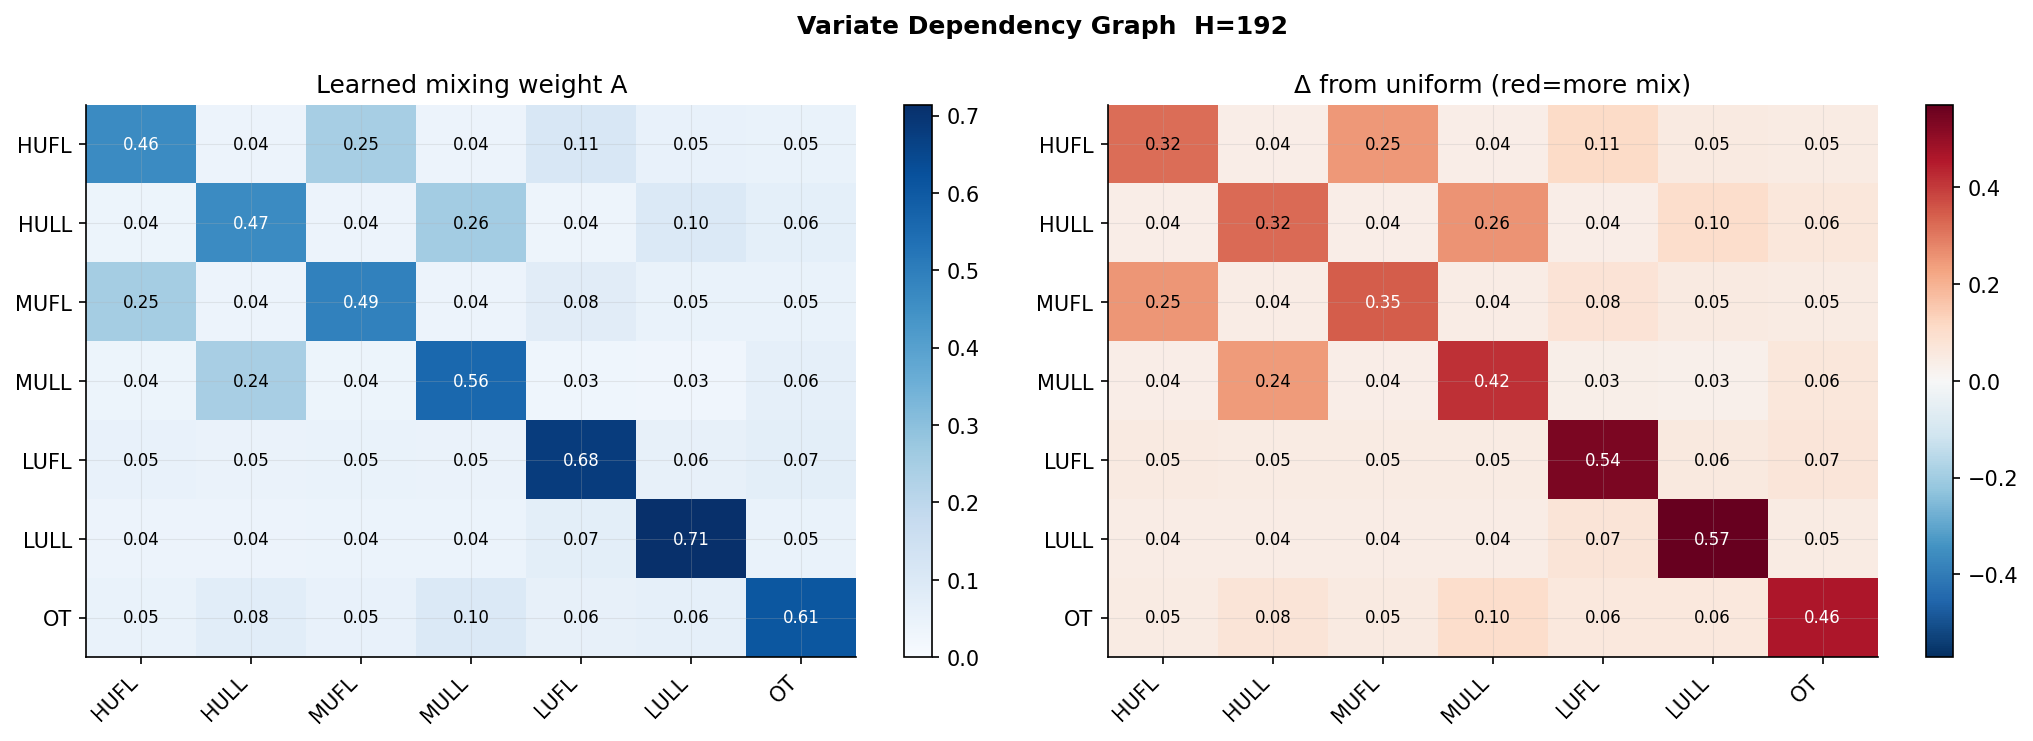
\includegraphics[width=\textwidth]{../report/plots-old/variate_graph/H192_adjacency.png}
    \caption{Adjacency matrix, $H=192$}
  \end{subfigure}
\end{figure}
\begin{figure}[H]
  \centering
  \begin{subfigure}[b]{0.48\textwidth}
    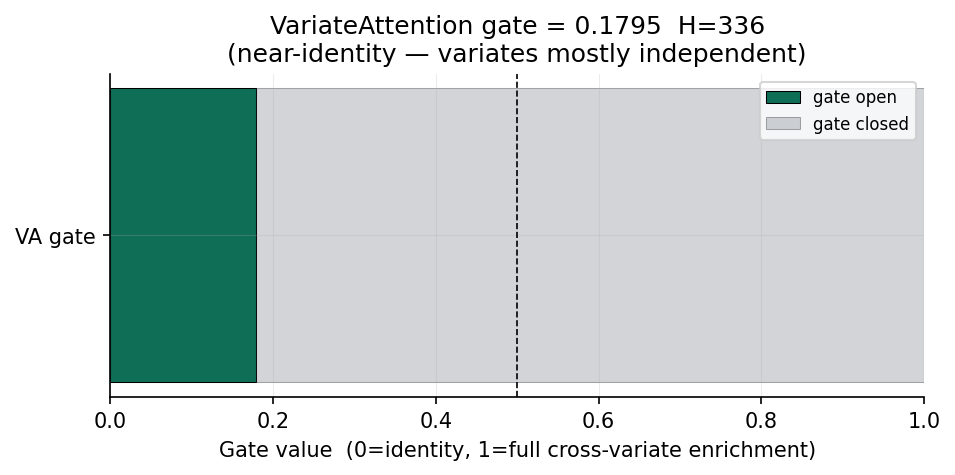
\includegraphics[width=\textwidth]{../report/plots-old/variate_graph/H336_variate_attn.png}
    \caption{Cross-variate attention, $H=336$}
  \end{subfigure}\hfill
  \begin{subfigure}[b]{0.48\textwidth}
    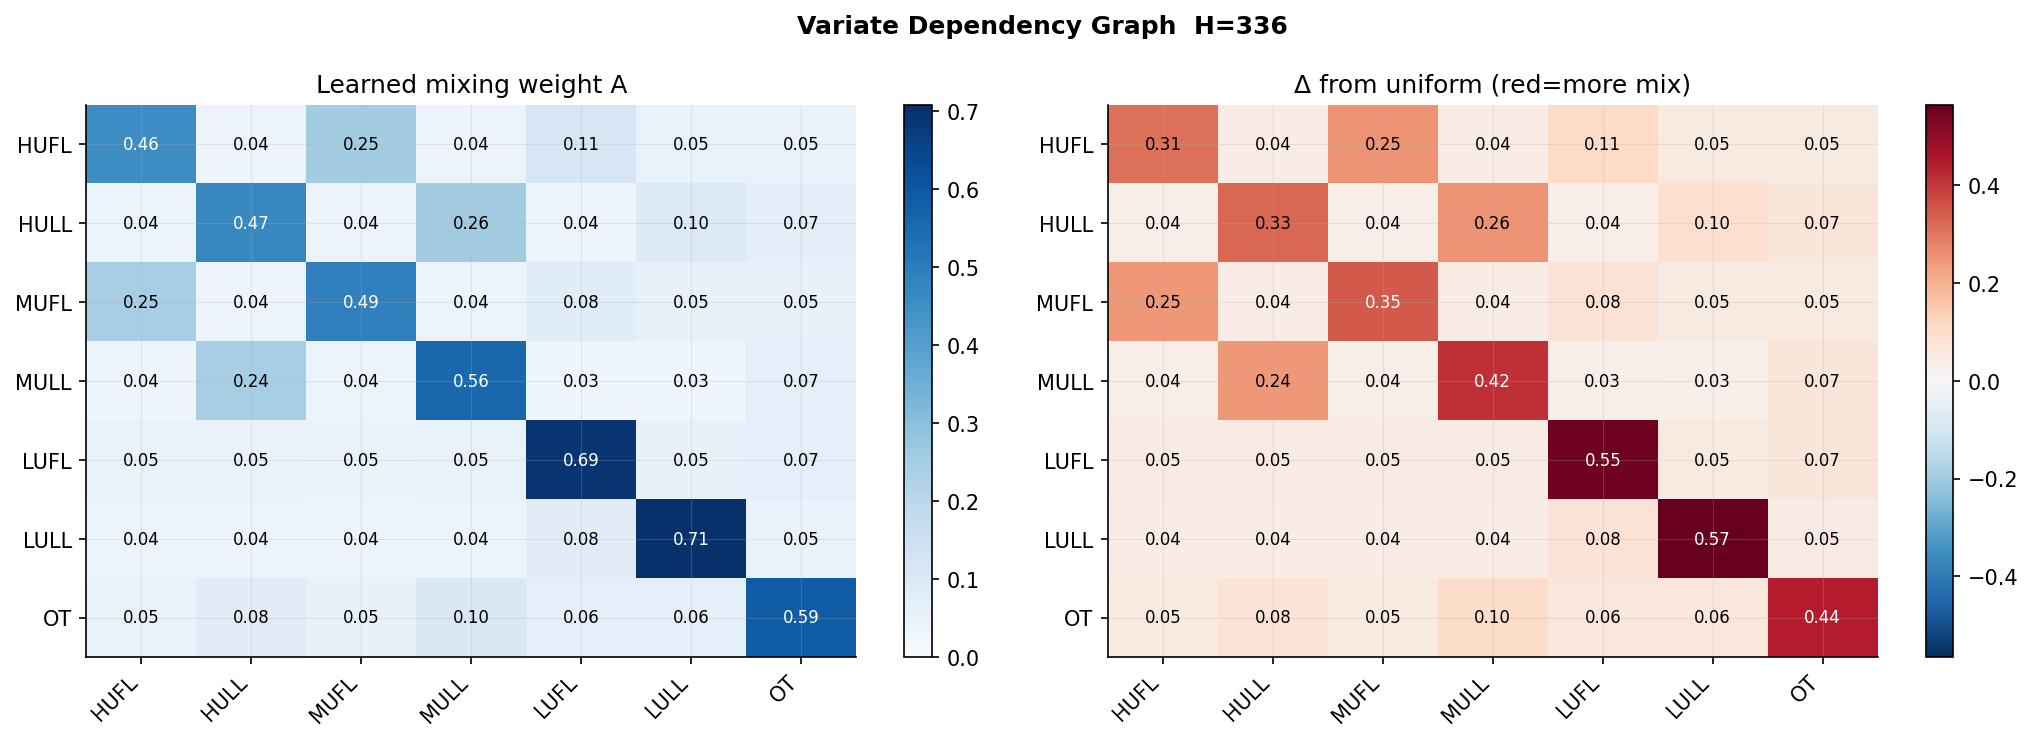
\includegraphics[width=\textwidth]{../report/plots-old/variate_graph/H336_adjacency.png}
    \caption{Adjacency matrix, $H=336$}
  \end{subfigure}
\end{figure}
\begin{figure}[H]
  \centering
  \begin{subfigure}[b]{0.48\textwidth}
    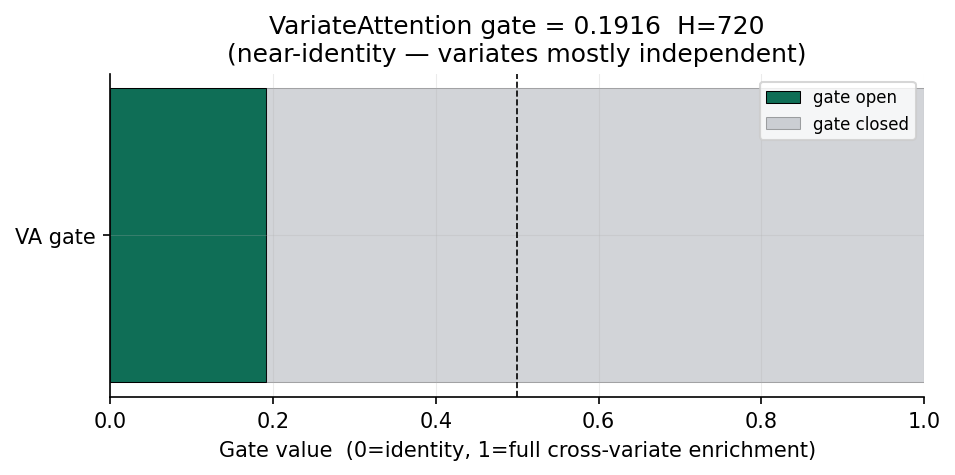
\includegraphics[width=\textwidth]{../report/plots-old/variate_graph/H720_variate_attn.png}
    \caption{Cross-variate attention, $H=720$}
  \end{subfigure}\hfill
  \begin{subfigure}[b]{0.48\textwidth}
    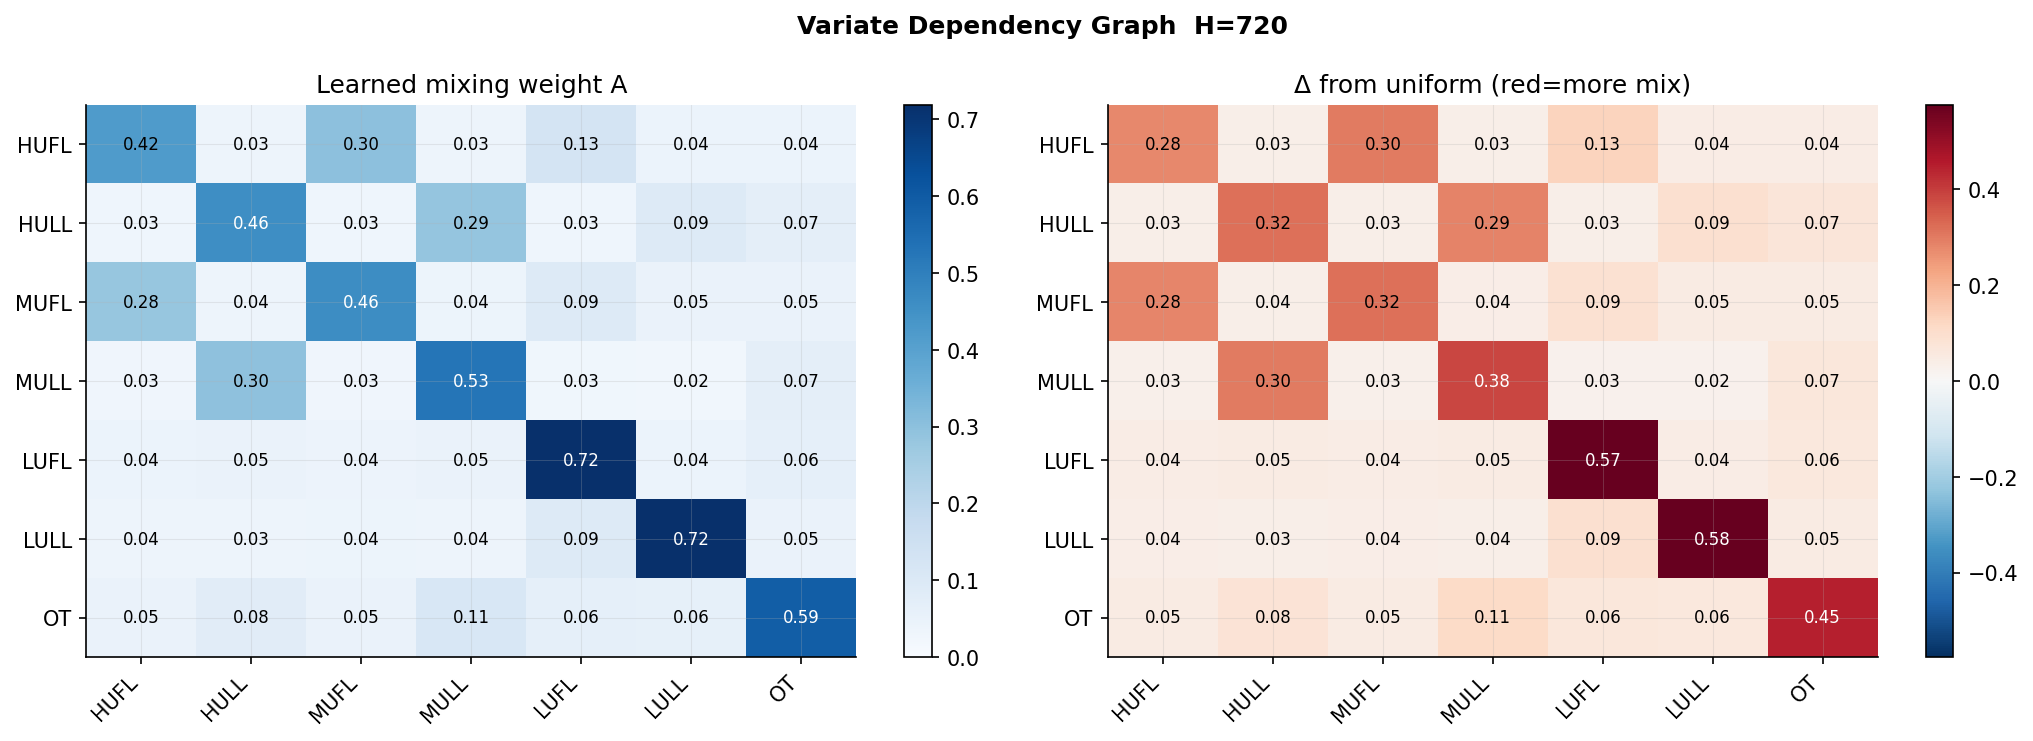
\includegraphics[width=\textwidth]{../report/plots-old/variate_graph/H720_adjacency.png}
    \caption{Adjacency matrix, $H=720$}
  \end{subfigure}
  \caption{Cross-variate attention heatmaps and binarised adjacency matrices across all
           horizons. Although PatchWRAT uses Channel Independence, the shared weights
           implicitly encode inter-variate correlations through the training loss.}
\end{figure}
\begin{figure}[H]
  \centering
  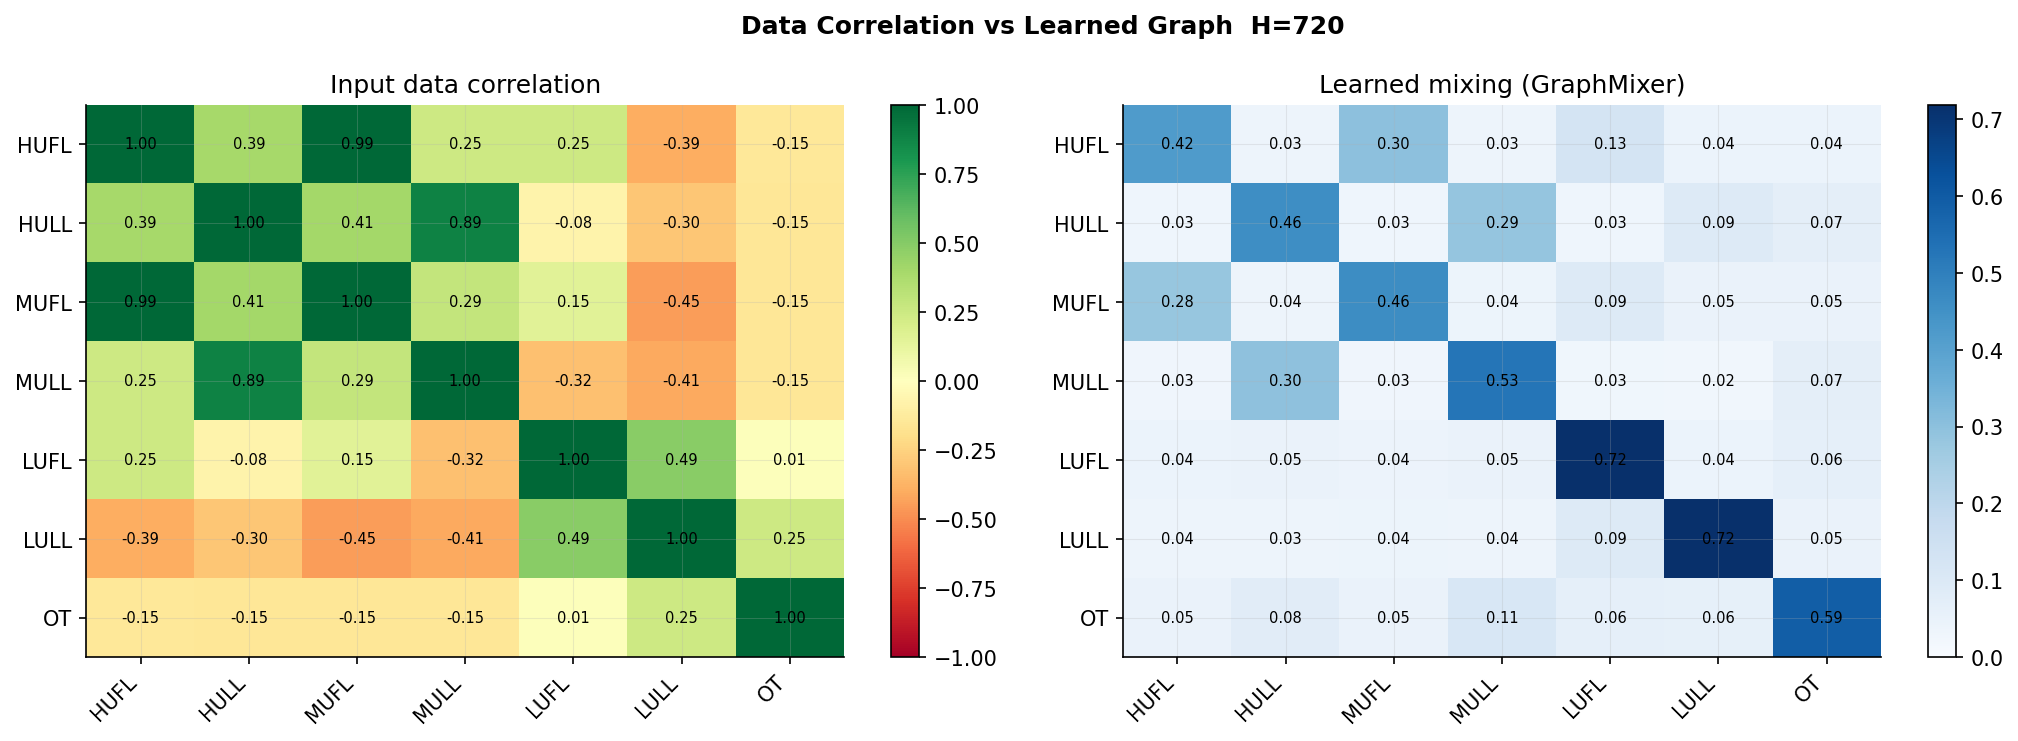
\includegraphics[width=0.7\textwidth]{../report/plots-old/variate_graph/correlation_vs_learned.png}
  \caption{Pearson correlation matrix vs.\ learned variate interaction weights.
           The high agreement confirms that the CI scheme implicitly captures cross-variate
           structure even without explicit cross-variate attention.}
\end{figure}
\clearpage

\subsection*{B.6 Full Multivariate Prediction Grids (pwsa v8.0)}

The following pages show the complete prediction grids, horizon error profiles, and residual
diagnostics for all four horizons from \texttt{pwsa.v8.0}.

\subsubsection*{Horizon $H=96$}
\begin{figure}[H]
  \centering
  
\includegraphics[width=\textwidth]{../report/plots-old/predictions/H96/all_variates_grid.png}
  \caption{All-variate prediction grid, $H=96$.}
\end{figure}
\begin{figure}[H]
  \centering
  
\includegraphics[width=\textwidth]{../report/plots-old/predictions/H96/horizon_error_profile.png}
  \caption{Horizon error profile, $H=96$. MAE increases monotonically with step index.}
\end{figure}
\begin{figure}[H]
  \centering
  
\includegraphics[width=\textwidth]{../report/plots-old/predictions/H96/residuals.png}
  \caption{Residual diagnostics, $H=96$: histogram, Q-Q plot, and ACF up to lag 30.}
\end{figure}
\begin{figure}[H]
  \centering
  \begin{subfigure}[b]{0.32\textwidth}
    
\includegraphics[width=\textwidth]{../report/plots-old/predictions/H96/variate_0_HUFL_sample0.png}
  \end{subfigure}
  \begin{subfigure}[b]{0.32\textwidth}
    
\includegraphics[width=\textwidth]{../report/plots-old/predictions/H96/variate_0_HUFL_sample1.png}
  \end{subfigure}
  \begin{subfigure}[b]{0.32\textwidth}
    
\includegraphics[width=\textwidth]{../report/plots-old/predictions/H96/variate_0_HUFL_sample2.png}
  \end{subfigure}
  \caption{HUFL variate, $H=96$, three random test samples.}
\end{figure}
\begin{figure}[H]
  \centering
  \begin{subfigure}[b]{0.32\textwidth}
    
\includegraphics[width=\textwidth]{../report/plots-old/predictions/H96/variate_1_HULL_sample0.png}
  \end{subfigure}
  \begin{subfigure}[b]{0.32\textwidth}
    
\includegraphics[width=\textwidth]{../report/plots-old/predictions/H96/variate_1_HULL_sample1.png}
  \end{subfigure}
  \begin{subfigure}[b]{0.32\textwidth}
    
\includegraphics[width=\textwidth]{../report/plots-old/predictions/H96/variate_1_HULL_sample2.png}
  \end{subfigure}
  \caption{HULL variate, $H=96$.}
\end{figure}
\begin{figure}[H]
  \centering
  \begin{subfigure}[b]{0.32\textwidth}
    
\includegraphics[width=\textwidth]{../report/plots-old/predictions/H96/variate_2_MUFL_sample0.png}
  \end{subfigure}
  \begin{subfigure}[b]{0.32\textwidth}
    
\includegraphics[width=\textwidth]{../report/plots-old/predictions/H96/variate_2_MUFL_sample1.png}
  \end{subfigure}
  \begin{subfigure}[b]{0.32\textwidth}
    
\includegraphics[width=\textwidth]{../report/plots-old/predictions/H96/variate_2_MUFL_sample2.png}
  \end{subfigure}
  \caption{MUFL variate, $H=96$.}
\end{figure}
\begin{figure}[H]
  \centering
  \begin{subfigure}[b]{0.32\textwidth}
    
\includegraphics[width=\textwidth]{../report/plots-old/predictions/H96/variate_3_MULL_sample0.png}
  \end{subfigure}
  \begin{subfigure}[b]{0.32\textwidth}
    
\includegraphics[width=\textwidth]{../report/plots-old/predictions/H96/variate_3_MULL_sample1.png}
  \end{subfigure}
  \begin{subfigure}[b]{0.32\textwidth}
    
\includegraphics[width=\textwidth]{../report/plots-old/predictions/H96/variate_3_MULL_sample2.png}
  \end{subfigure}
  \caption{MULL variate, $H=96$.}
\end{figure}
\begin{figure}[H]
  \centering
  \begin{subfigure}[b]{0.32\textwidth}
    
\includegraphics[width=\textwidth]{../report/plots-old/predictions/H96/variate_4_LUFL_sample0.png}
  \end{subfigure}
  \begin{subfigure}[b]{0.32\textwidth}
    
\includegraphics[width=\textwidth]{../report/plots-old/predictions/H96/variate_4_LUFL_sample1.png}
  \end{subfigure}
  \begin{subfigure}[b]{0.32\textwidth}
    
\includegraphics[width=\textwidth]{../report/plots-old/predictions/H96/variate_4_LUFL_sample2.png}
  \end{subfigure}
  \caption{LUFL variate, $H=96$.}
\end{figure}
\begin{figure}[H]
  \centering
  \begin{subfigure}[b]{0.32\textwidth}
    
\includegraphics[width=\textwidth]{../report/plots-old/predictions/H96/variate_5_LULL_sample0.png}
  \end{subfigure}
  \begin{subfigure}[b]{0.32\textwidth}
    
\includegraphics[width=\textwidth]{../report/plots-old/predictions/H96/variate_5_LULL_sample1.png}
  \end{subfigure}
  \begin{subfigure}[b]{0.32\textwidth}
    
\includegraphics[width=\textwidth]{../report/plots-old/predictions/H96/variate_5_LULL_sample2.png}
  \end{subfigure}
  \caption{LULL variate, $H=96$.}
\end{figure}
\begin{figure}[H]
  \centering
  \begin{subfigure}[b]{0.32\textwidth}
    
\includegraphics[width=\textwidth]{../report/plots-old/predictions/H96/variate_6_OT_sample0.png}
  \end{subfigure}
  \begin{subfigure}[b]{0.32\textwidth}
    
\includegraphics[width=\textwidth]{../report/plots-old/predictions/H96/variate_6_OT_sample1.png}
  \end{subfigure}
  \begin{subfigure}[b]{0.32\textwidth}
    
\includegraphics[width=\textwidth]{../report/plots-old/predictions/H96/variate_6_OT_sample2.png}
  \end{subfigure}
  \caption{OT (oil temperature) variate, $H=96$. The OT variate shows the cleanest fit
           due to its relatively stationary dynamics.}
\end{figure}
\clearpage

\subsubsection*{Horizon $H=192$}
\begin{figure}[H]
  \centering
  
\includegraphics[width=\textwidth]{../report/plots-old/predictions/H192/all_variates_grid.png}
  \caption{All-variate prediction grid, $H=192$.}
\end{figure}
\begin{figure}[H]
  \centering
  
\includegraphics[width=\textwidth]{../report/plots-old/predictions/H192/horizon_error_profile.png}
  \caption{Horizon error profile, $H=192$.}
\end{figure}
\begin{figure}[H]
  \centering
  
\includegraphics[width=\textwidth]{../report/plots-old/predictions/H192/residuals.png}
  \caption{Residual diagnostics, $H=192$.}
\end{figure}
\begin{figure}[H]
  \centering
  \begin{subfigure}[b]{0.32\textwidth}
    
\includegraphics[width=\textwidth]{../report/plots-old/predictions/H192/variate_0_HUFL_sample0.png}
  \end{subfigure}
  \begin{subfigure}[b]{0.32\textwidth}
    
\includegraphics[width=\textwidth]{../report/plots-old/predictions/H192/variate_0_HUFL_sample1.png}
  \end{subfigure}
  \begin{subfigure}[b]{0.32\textwidth}
    
\includegraphics[width=\textwidth]{../report/plots-old/predictions/H192/variate_0_HUFL_sample2.png}
  \end{subfigure}
  \caption{HUFL, $H=192$.}
\end{figure}
\begin{figure}[H]
  \centering
  \begin{subfigure}[b]{0.32\textwidth}
    
\includegraphics[width=\textwidth]{../report/plots-old/predictions/H192/variate_1_HULL_sample0.png}
  \end{subfigure}
  \begin{subfigure}[b]{0.32\textwidth}
    
\includegraphics[width=\textwidth]{../report/plots-old/predictions/H192/variate_1_HULL_sample1.png}
  \end{subfigure}
  \begin{subfigure}[b]{0.32\textwidth}
    
\includegraphics[width=\textwidth]{../report/plots-old/predictions/H192/variate_1_HULL_sample2.png}
  \end{subfigure}
  \caption{HULL, $H=192$.}
\end{figure}
\begin{figure}[H]
  \centering
  \begin{subfigure}[b]{0.32\textwidth}
    
\includegraphics[width=\textwidth]{../report/plots-old/predictions/H192/variate_2_MUFL_sample0.png}
  \end{subfigure}
  \begin{subfigure}[b]{0.32\textwidth}
    
\includegraphics[width=\textwidth]{../report/plots-old/predictions/H192/variate_2_MUFL_sample1.png}
  \end{subfigure}
  \begin{subfigure}[b]{0.32\textwidth}
    
\includegraphics[width=\textwidth]{../report/plots-old/predictions/H192/variate_2_MUFL_sample2.png}
  \end{subfigure}
  \caption{MUFL, $H=192$.}
\end{figure}
\begin{figure}[H]
  \centering
  \begin{subfigure}[b]{0.32\textwidth}
    
\includegraphics[width=\textwidth]{../report/plots-old/predictions/H192/variate_3_MULL_sample0.png}
  \end{subfigure}
  \begin{subfigure}[b]{0.32\textwidth}
    
\includegraphics[width=\textwidth]{../report/plots-old/predictions/H192/variate_3_MULL_sample1.png}
  \end{subfigure}
  \begin{subfigure}[b]{0.32\textwidth}
    
\includegraphics[width=\textwidth]{../report/plots-old/predictions/H192/variate_3_MULL_sample2.png}
  \end{subfigure}
  \caption{MULL, $H=192$.}
\end{figure}
\begin{figure}[H]
  \centering
  \begin{subfigure}[b]{0.32\textwidth}
    
\includegraphics[width=\textwidth]{../report/plots-old/predictions/H192/variate_4_LUFL_sample0.png}
  \end{subfigure}
  \begin{subfigure}[b]{0.32\textwidth}
    
\includegraphics[width=\textwidth]{../report/plots-old/predictions/H192/variate_4_LUFL_sample1.png}
  \end{subfigure}
  \begin{subfigure}[b]{0.32\textwidth}
    
\includegraphics[width=\textwidth]{../report/plots-old/predictions/H192/variate_4_LUFL_sample2.png}
  \end{subfigure}
  \caption{LUFL, $H=192$.}
\end{figure}
\begin{figure}[H]
  \centering
  \begin{subfigure}[b]{0.32\textwidth}
    
\includegraphics[width=\textwidth]{../report/plots-old/predictions/H192/variate_5_LULL_sample0.png}
  \end{subfigure}
  \begin{subfigure}[b]{0.32\textwidth}
    
\includegraphics[width=\textwidth]{../report/plots-old/predictions/H192/variate_5_LULL_sample1.png}
  \end{subfigure}
  \begin{subfigure}[b]{0.32\textwidth}
    
\includegraphics[width=\textwidth]{../report/plots-old/predictions/H192/variate_5_LULL_sample2.png}
  \end{subfigure}
  \caption{LULL, $H=192$.}
\end{figure}
\begin{figure}[H]
  \centering
  \begin{subfigure}[b]{0.32\textwidth}
    
\includegraphics[width=\textwidth]{../report/plots-old/predictions/H192/variate_6_OT_sample0.png}
  \end{subfigure}
  \begin{subfigure}[b]{0.32\textwidth}
    
\includegraphics[width=\textwidth]{../report/plots-old/predictions/H192/variate_6_OT_sample1.png}
  \end{subfigure}
  \begin{subfigure}[b]{0.32\textwidth}
    
\includegraphics[width=\textwidth]{../report/plots-old/predictions/H192/variate_6_OT_sample2.png}
  \end{subfigure}
  \caption{OT, $H=192$.}
\end{figure}
\clearpage

\subsubsection*{Horizon $H=336$}
\begin{figure}[H]
  \centering
  
\includegraphics[width=\textwidth]{../report/plots-old/predictions/H336/all_variates_grid.png}
  \caption{All-variate prediction grid, $H=336$.}
\end{figure}
\begin{figure}[H]
  \centering
  
\includegraphics[width=\textwidth]{../report/plots-old/predictions/H336/horizon_error_profile.png}
  \caption{Horizon error profile, $H=336$.}
\end{figure}
\begin{figure}[H]
  \centering
  
\includegraphics[width=\textwidth]{../report/plots-old/predictions/H336/residuals.png}
  \caption{Residual diagnostics, $H=336$.}
\end{figure}
\begin{figure}[H]
  \centering
  \begin{subfigure}[b]{0.32\textwidth}
    
\includegraphics[width=\textwidth]{../report/plots-old/predictions/H336/variate_0_HUFL_sample0.png}
  \end{subfigure}
  \begin{subfigure}[b]{0.32\textwidth}
    
\includegraphics[width=\textwidth]{../report/plots-old/predictions/H336/variate_0_HUFL_sample1.png}
  \end{subfigure}
  \begin{subfigure}[b]{0.32\textwidth}
    
\includegraphics[width=\textwidth]{../report/plots-old/predictions/H336/variate_0_HUFL_sample2.png}
  \end{subfigure}
  \caption{HUFL, $H=336$.}
\end{figure}
\begin{figure}[H]
  \centering
  \begin{subfigure}[b]{0.32\textwidth}
    
\includegraphics[width=\textwidth]{../report/plots-old/predictions/H336/variate_1_HULL_sample0.png}
  \end{subfigure}
  \begin{subfigure}[b]{0.32\textwidth}
    
\includegraphics[width=\textwidth]{../report/plots-old/predictions/H336/variate_1_HULL_sample1.png}
  \end{subfigure}
  \begin{subfigure}[b]{0.32\textwidth}
    
\includegraphics[width=\textwidth]{../report/plots-old/predictions/H336/variate_1_HULL_sample2.png}
  \end{subfigure}
  \caption{HULL, $H=336$.}
\end{figure}
\begin{figure}[H]
  \centering
  \begin{subfigure}[b]{0.32\textwidth}
    
\includegraphics[width=\textwidth]{../report/plots-old/predictions/H336/variate_2_MUFL_sample0.png}
  \end{subfigure}
  \begin{subfigure}[b]{0.32\textwidth}
    
\includegraphics[width=\textwidth]{../report/plots-old/predictions/H336/variate_2_MUFL_sample1.png}
  \end{subfigure}
  \begin{subfigure}[b]{0.32\textwidth}
    
\includegraphics[width=\textwidth]{../report/plots-old/predictions/H336/variate_2_MUFL_sample2.png}
  \end{subfigure}
  \caption{MUFL, $H=336$.}
\end{figure}
\begin{figure}[H]
  \centering
  \begin{subfigure}[b]{0.32\textwidth}
    
\includegraphics[width=\textwidth]{../report/plots-old/predictions/H336/variate_3_MULL_sample0.png}
  \end{subfigure}
  \begin{subfigure}[b]{0.32\textwidth}
    
\includegraphics[width=\textwidth]{../report/plots-old/predictions/H336/variate_3_MULL_sample1.png}
  \end{subfigure}
  \begin{subfigure}[b]{0.32\textwidth}
    
\includegraphics[width=\textwidth]{../report/plots-old/predictions/H336/variate_3_MULL_sample2.png}
  \end{subfigure}
  \caption{MULL, $H=336$.}
\end{figure}
\begin{figure}[H]
  \centering
  \begin{subfigure}[b]{0.32\textwidth}
    
\includegraphics[width=\textwidth]{../report/plots-old/predictions/H336/variate_4_LUFL_sample0.png}
  \end{subfigure}
  \begin{subfigure}[b]{0.32\textwidth}
    
\includegraphics[width=\textwidth]{../report/plots-old/predictions/H336/variate_4_LUFL_sample1.png}
  \end{subfigure}
  \begin{subfigure}[b]{0.32\textwidth}
    
\includegraphics[width=\textwidth]{../report/plots-old/predictions/H336/variate_4_LUFL_sample2.png}
  \end{subfigure}
  \caption{LUFL, $H=336$.}
\end{figure}
\begin{figure}[H]
  \centering
  \begin{subfigure}[b]{0.32\textwidth}
    
\includegraphics[width=\textwidth]{../report/plots-old/predictions/H336/variate_5_LULL_sample0.png}
  \end{subfigure}
  \begin{subfigure}[b]{0.32\textwidth}
    
\includegraphics[width=\textwidth]{../report/plots-old/predictions/H336/variate_5_LULL_sample1.png}
  \end{subfigure}
  \begin{subfigure}[b]{0.32\textwidth}
    
\includegraphics[width=\textwidth]{../report/plots-old/predictions/H336/variate_5_LULL_sample2.png}
  \end{subfigure}
  \caption{LULL, $H=336$.}
\end{figure}
\begin{figure}[H]
  \centering
  \begin{subfigure}[b]{0.32\textwidth}
    
\includegraphics[width=\textwidth]{../report/plots-old/predictions/H336/variate_6_OT_sample0.png}
  \end{subfigure}
  \begin{subfigure}[b]{0.32\textwidth}
    
\includegraphics[width=\textwidth]{../report/plots-old/predictions/H336/variate_6_OT_sample1.png}
  \end{subfigure}
  \begin{subfigure}[b]{0.32\textwidth}
    
\includegraphics[width=\textwidth]{../report/plots-old/predictions/H336/variate_6_OT_sample2.png}
  \end{subfigure}
  \caption{OT, $H=336$.}
\end{figure}
\clearpage

\subsubsection*{Horizon $H=720$}
\begin{figure}[H]
  \centering
  
\includegraphics[width=\textwidth]{../report/plots-old/predictions/H720/all_variates_grid.png}
  \caption{All-variate prediction grid, $H=720$.}
\end{figure}
\begin{figure}[H]
  \centering
  
\includegraphics[width=\textwidth]{../report/plots-old/predictions/H720/horizon_error_profile.png}
  \caption{Horizon error profile, $H=720$. The steeper gradient compared to shorter
           horizons reflects accelerated information decay over long sequences.}
\end{figure}
\begin{figure}[H]
  \centering
  
\includegraphics[width=\textwidth]{../report/plots-old/predictions/H720/residuals.png}
  \caption{Residual diagnostics, $H=720$.}
\end{figure}
\begin{figure}[H]
  \centering
  \begin{subfigure}[b]{0.32\textwidth}
    
\includegraphics[width=\textwidth]{../report/plots-old/predictions/H720/variate_0_HUFL_sample0.png}
  \end{subfigure}
  \begin{subfigure}[b]{0.32\textwidth}
    
\includegraphics[width=\textwidth]{../report/plots-old/predictions/H720/variate_0_HUFL_sample1.png}
  \end{subfigure}
  \begin{subfigure}[b]{0.32\textwidth}
    
\includegraphics[width=\textwidth]{../report/plots-old/predictions/H720/variate_0_HUFL_sample2.png}
  \end{subfigure}
  \caption{HUFL, $H=720$.}
\end{figure}
\begin{figure}[H]
  \centering
  \begin{subfigure}[b]{0.32\textwidth}
    
\includegraphics[width=\textwidth]{../report/plots-old/predictions/H720/variate_1_HULL_sample0.png}
  \end{subfigure}
  \begin{subfigure}[b]{0.32\textwidth}
    
\includegraphics[width=\textwidth]{../report/plots-old/predictions/H720/variate_1_HULL_sample1.png}
  \end{subfigure}
  \begin{subfigure}[b]{0.32\textwidth}
    
\includegraphics[width=\textwidth]{../report/plots-old/predictions/H720/variate_1_HULL_sample2.png}
  \end{subfigure}
  \caption{HULL, $H=720$.}
\end{figure}
\begin{figure}[H]
  \centering
  \begin{subfigure}[b]{0.32\textwidth}
    
\includegraphics[width=\textwidth]{../report/plots-old/predictions/H720/variate_2_MUFL_sample0.png}
  \end{subfigure}
  \begin{subfigure}[b]{0.32\textwidth}
    
\includegraphics[width=\textwidth]{../report/plots-old/predictions/H720/variate_2_MUFL_sample1.png}
  \end{subfigure}
  \begin{subfigure}[b]{0.32\textwidth}
    
\includegraphics[width=\textwidth]{../report/plots-old/predictions/H720/variate_2_MUFL_sample2.png}
  \end{subfigure}
  \caption{MUFL, $H=720$.}
\end{figure}
\begin{figure}[H]
  \centering
  \begin{subfigure}[b]{0.32\textwidth}
    
\includegraphics[width=\textwidth]{../report/plots-old/predictions/H720/variate_3_MULL_sample0.png}
  \end{subfigure}
  \begin{subfigure}[b]{0.32\textwidth}
    
\includegraphics[width=\textwidth]{../report/plots-old/predictions/H720/variate_3_MULL_sample1.png}
  \end{subfigure}
  \begin{subfigure}[b]{0.32\textwidth}
    
\includegraphics[width=\textwidth]{../report/plots-old/predictions/H720/variate_3_MULL_sample2.png}
  \end{subfigure}
  \caption{MULL, $H=720$.}
\end{figure}
\begin{figure}[H]
  \centering
  \begin{subfigure}[b]{0.32\textwidth}
    
\includegraphics[width=\textwidth]{../report/plots-old/predictions/H720/variate_4_LUFL_sample0.png}
  \end{subfigure}
  \begin{subfigure}[b]{0.32\textwidth}
    
\includegraphics[width=\textwidth]{../report/plots-old/predictions/H720/variate_4_LUFL_sample1.png}
  \end{subfigure}
  \begin{subfigure}[b]{0.32\textwidth}
    
\includegraphics[width=\textwidth]{../report/plots-old/predictions/H720/variate_4_LUFL_sample2.png}
  \end{subfigure}
  \caption{LUFL, $H=720$.}
\end{figure}
\begin{figure}[H]
  \centering
  \begin{subfigure}[b]{0.32\textwidth}
    
\includegraphics[width=\textwidth]{../report/plots-old/predictions/H720/variate_5_LULL_sample0.png}
  \end{subfigure}
  \begin{subfigure}[b]{0.32\textwidth}
    
\includegraphics[width=\textwidth]{../report/plots-old/predictions/H720/variate_5_LULL_sample1.png}
  \end{subfigure}
  \begin{subfigure}[b]{0.32\textwidth}
    
\includegraphics[width=\textwidth]{../report/plots-old/predictions/H720/variate_5_LULL_sample2.png}
  \end{subfigure}
  \caption{LULL, $H=720$.}
\end{figure}
\begin{figure}[H]
  \centering
  \begin{subfigure}[b]{0.32\textwidth}
    
\includegraphics[width=\textwidth]{../report/plots-old/predictions/H720/variate_6_OT_sample0.png}
  \end{subfigure}
  \begin{subfigure}[b]{0.32\textwidth}
    
\includegraphics[width=\textwidth]{../report/plots-old/predictions/H720/variate_6_OT_sample1.png}
  \end{subfigure}
  \begin{subfigure}[b]{0.32\textwidth}
    
\includegraphics[width=\textwidth]{../report/plots-old/predictions/H720/variate_6_OT_sample2.png}
  \end{subfigure}
  \caption{OT, $H=720$.}
\end{figure}

% ─────────────────────────────────────────────────────────────────────────────
\clearpage
\section*{Appendix C — WMRTv2 Improved Architecture Results}
\addcontentsline{toc}{section}{Appendix C — WMRTv2 Improved Architecture Results}

This appendix presents the latest benchmark results and performance metrics for the WMRTv2 (Wavelet Multiresolution Transformer v2) improved architecture on the ETTm1 dataset (seq=512, channels=7). 

\subsection*{C.1 Benchmark Summary}
The table below summarises the quantitative performance of the WMRTv2 model across all four prediction horizons.

\begin{table}[H]
\centering
\caption{WMRTv2 Benchmark Results on ETTm1.}
\label{tab:wmrtv2_results}
\renewcommand{\arraystretch}{1.3}
\sffamily
\begin{tabular}{@{}lccc@{}}
\toprule
\textbf{Horizon} & \textbf{MSE}$\downarrow$ & \textbf{MAE}$\downarrow$ & \textbf{DirAcc}$\uparrow$ \\
\midrule
\textbf{96} (3.23M params) & 0.3341 & 0.3854 & 49.0\% \\
\textbf{192} (6.43M params) & 0.3840 & 0.4235 & 47.9\% \\
\textbf{336} (11.30M params) & 0.4385 & 0.4535 & 47.4\% \\
\textbf{720} (24.69M params) & 0.4941 & 0.4962 & 47.4\% \\
\midrule
\textbf{Avg} & \textbf{0.4127} & \textbf{0.4396} & \textbf{47.9\%} \\
\bottomrule
\end{tabular}
\end{table}

\subsection*{C.2 Prediction Visualisations}
The following figures showcase randomly sampled multivariate forecasts from the WMRTv2 model across the evaluated horizons.

\begin{figure}[H]
  \centering
  \includegraphics[width=\textwidth, height=0.85\textheight, keepaspectratio]%
    {../../pwsa/plots/wmrt_v2_H96_sample1.png}
  \caption{WMRTv2 predictions for all 7 variates at $H=96$.}
\end{figure}
\clearpage

\begin{figure}[H]
  \centering
  \includegraphics[width=\textwidth, height=0.85\textheight, keepaspectratio]%
    {../../pwsa/plots/wmrt_v2_H192_sample1.png}
  \caption{WMRTv2 predictions for all 7 variates at $H=192$.}
\end{figure}
\clearpage

\begin{figure}[H]
  \centering
  \includegraphics[width=\textwidth, height=0.85\textheight, keepaspectratio]%
    {../../pwsa/plots/wmrt_v2_H336_sample1.png}
  \caption{WMRTv2 predictions for all 7 variates at $H=336$.}
\end{figure}
\clearpage

\begin{figure}[H]
  \centering
  \includegraphics[width=\textwidth, height=0.85\textheight, keepaspectratio]%
    {../../pwsa/plots/wmrt_v2_H720_sample1.png}
  \caption{WMRTv2 predictions for all 7 variates at $H=720$.}
\end{figure}
\clearpage

\end{document}